% Tento soubor nahraďte vlastním souborem s obsahem práce.
%=========================================================================
% Autoři: Michal Bidlo, Bohuslav Křena, Jaroslav Dytrych, Petr Veigend a Adam Herout 2019


\setcounter{tocdepth}{1} 

\definecolor{ao}{rgb}{0.0, 0.5, 0.0}
\lstset{language=C,
  aboveskip=3mm,
  belowskip=3mm,
  showstringspaces=false,
  columns=flexible,
  basicstyle={\small\ttfamily},
  numbers=none,
  numberstyle=\tiny\color{gray},
  keywordstyle=\color{blue},
  commentstyle=\color{ao},
  stringstyle=\color{mauve},
  breaklines=true,
  breakatwhitespace=true,
  tabsize=3
}

\chapter{Úvod}
Částicové systémy se obvykle využívají pro zobrazení efektů, jako jsou oheň, mlha nebo tekutiny. Pro zobrazení v~reálném čase však musí být částice velmi jednoduché. \textbf{Light field} je metoda vykreslování pomocí obrázku, která umožňuje zachytit světlo vycházející z~objektu a následně jej reprodukovat ze všech úhlů, ze kterých byl zachycen.   

Tato práce se věnuje návrhu, implementaci a testování metody tvorby částicových efektů, kde je textura jednotlivých částic vytvořena pomocí light fieldu. Částice tak mohou působit jako třírozměrné objekty, i když se jedná o~pouhé \textbf{billboardy}, jak je například možné pozorovat na Obrázku \ref{fig:uvod_example}.

Výstupem práce je nástroj, který demonstruje různá použití této metody a následná měření porovnávající tuto metodu se standardním vykreslováním. Nástroj také implementuje různá rozšíření, jako například dynamické dogenerovávání light fieldu za běhu podle potřebných úhlů pohledu nebo větší množství light fieldů pro jednu částici.

Kapitola \emph{Teorie} se věnuje popisu pojmů jako jsou například light field nebo billboard. V~kapitole \emph{Návrh} je popsána navrhovaná metoda, architektura a metodika měření. Kapitola \emph{Implementace} se věnuje konkréktní realizaci a v~kapitole \emph{Měření} se nachází výstup a analýza měření. Poslední kapitola \emph{Závěr} shrnuje výstupy práce. 

\begin{figure}[H]
	\centering
	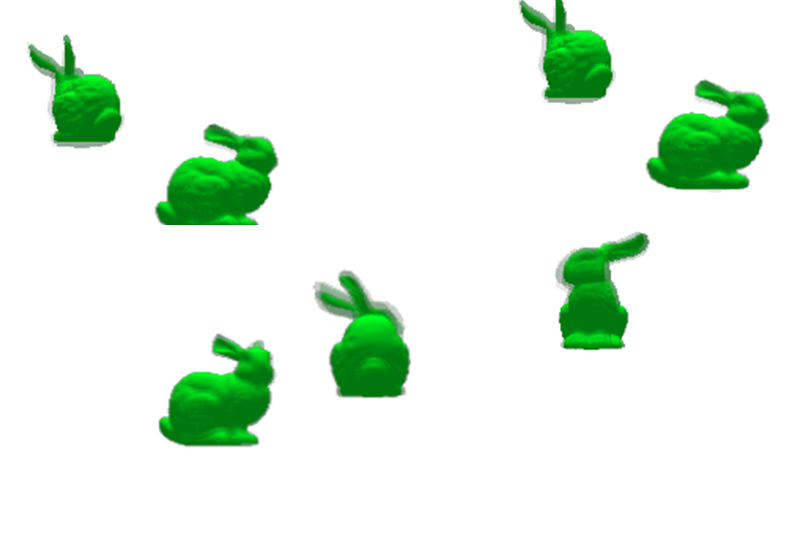
\includegraphics[width=0.4\textwidth]{obrazky-figures/particles_fake.png}
	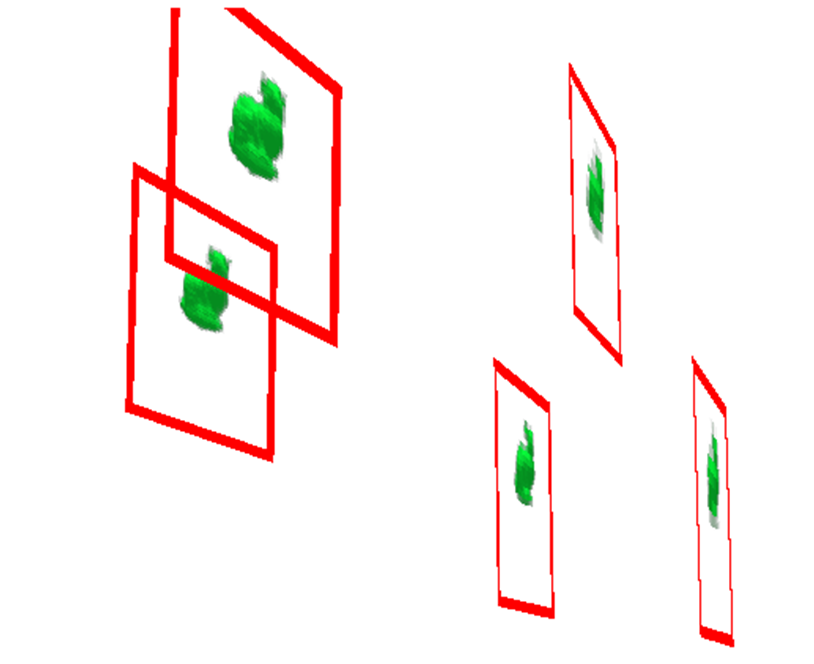
\includegraphics[width=0.4\textwidth]{obrazky-figures/particles_true.png}
	\caption{Příklad částicového efektu, kde jsou jednotlivé částice pouze dvourozměrné čtverce a jejich textura je vytvořena pomocí light fieldu. Na levém obrázku je billboarding zapnutý, na pravém vypnutý a částice jsou ohraničeny.}
	\label{fig:uvod_example}
\end{figure}
\chapter{Teorie}
Tato kapitola se věnuje třem základním fenoménům, které byly použity při tvorbě práce. Billboarding je metoda natáčení čtverce s~texturou kolmo ke kameře. Částicový systém je způsob, jak modelovat objekty či jevy skládající se z~velkého množství malých autonomních objektů. V~této kapitole jsou popsány způsoby simulace a možné použití čáticových systémů. Light field je způsob parametrizace světla, které vyzařuje objekt a light field rendering je metoda zobrazení tohoto objektu ze zachyceného světla. Dále je v~kapitole také popsáno mipmapování, které je především relevantní pro implementaci a měření.
\section{Billboard}
Billboarding je metoda natáčení čtverce v~prostoru v~závislosti na kameře. Takový čtverec se nazývá billboard. Je pokryt texturou, která může být místy částečně nebo zcela průhledná. V~praxi se používá k~zobrazení efektů nebo objektů, které je neefektivní vykreslovat v~reálném čase, například vegetace, mraky či kouř (jak je například zobrazeno na obrázku \ref{fig:billboard_expample}). Díky nízkým výkonnostním nárokům lze billboardy také využít jako jednotlivé částice v~částicových systémech. Tato metoda je popsána knize \emph{Real-Time Rendering Fourth Edition}  \cite[kapitola~13.6]{ller2018real}, kde autoři popisují její princip a realizaci. 
\begin{figure}[H]
	\centering
	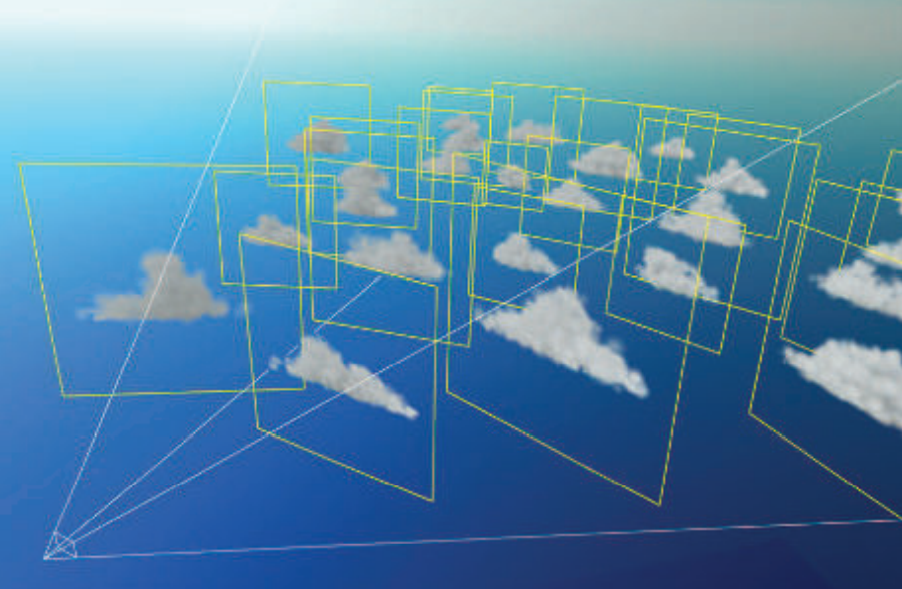
\includegraphics[width=0.65\textwidth]{obrazky-figures/test4.png}
	\caption{Příklad zobrazení efektu mraků pomocí textury nanesené na billboard. Převzato z~knihy \emph{Real-Time Rendering Fourth Edition} \cite[kapitola 13.6]{ller2018real}. }
	\label{fig:billboard_expample}
\end{figure}

Billboard je rotován směrem ke kameře pomocí rotační matice \(M\). Jednotlivé vertexy jsou obvykle rotovány podle středu obdélníku. Rotační matice \(M\) je vytvořena pomocí vektoru \(u\) směřujícím vzhůru a normály povrchu billboardu \(n\). Vektory \(u\) a \(n\) jsou normalizované, a tvoří tak ortonormální bázi povrchu billboardu. Jeden z~těchto vektorů je fixovaný na kameru. Pokud druhý vektor není na fixovaný vektor kolmý, tak je nutné jej upravit.

U~obou metod je nedříve nutné vytvořit pravý vektor \(r\), který směřuje k~pravému kraji billboardu. Lze jej vypočítat podle rovnice \ref{eq:1}.
\begin{equation}
r = u~\times n
\label{eq:1}
\end{equation}

Vektor \(r\) je poté nutné normalizovat. Nyní lze upravit nefixovaný vektor \(u\) nebo \(n\) tak, aby byl kolmý s~fixovaným. Pokud je fixovaný vektor \(n\), lze nový vektor \(u'\) spočítat podle rovnice \ref{eq:2}.
\begin{equation}
u' = n \times r
\label{eq:2}
\end{equation}
Postup vytváření vektoru \(u'\) je znázorněn na obrázku \ref{fig:rotation_expample}. Pokud je fixovaný vektor $u$, tak lze nový vektor $n'$ spočítat rovnicí \ref{eq:3}.
\begin{equation}
n' = r \times
u~\label{eq:3}
\end{equation}
Nově spočítaný vektor je nutné normalizovat. Konečná rotační matice pro fixovaný vektor n   vypadá takto:
\[M = (r, u', n)\]

\begin{figure}[H]
	\centering
	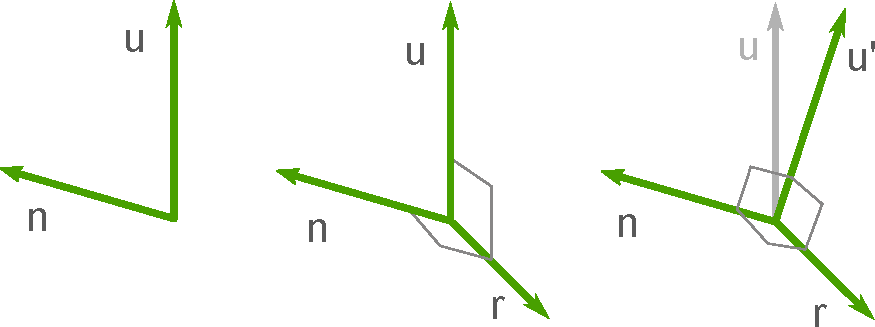
\includegraphics[width=0.7\textwidth]{obrazky-figures/billboarding_rot.pdf}
	\caption{Znázornění postupu výpočtu vektoru \(u'\) popsaný rovnicí \ref{eq:2}. Inspirováno obrázkem z~knihy \emph{Real-Time Rendering Fourth Edition} \cite[kapitola 13.6]{ller2018real}. }
	\label{fig:rotation_expample}
\end{figure}
\subsection{Kamerou orientovaný billboard}
\label{sec:camoriented_billboard}
Jedna z~variant billboardu je kamerou orientovaný billboard. V~této variantě je billboard orientován tak, aby byl vždy souběžný s~pohledovou rovinou. Normála billboardu je rovna negaci normály pohledové roviny a up vektor je přímo roven up vektoru kamery. Obě tyto hodnoty jsou konstantní a je tak možné je předpočítat a použít pro větší množství billboardů. Vektory \(u\) a \(n\) jsou na sebe kolmé, stačí tedy jen dopočítat vektor \(r\). 

Tato varianta billboardu je tedy vždy orientována směrem ke kameře nezávisle na okolním světě, což je znázorněno na obrázku \ref{fig:billboard_camera_aligned}. Používá se často například pro zobrazení textu nebo pro zobrazení jednotlivých částic v~částicovém systému.
\begin{figure}[H]
	\centering
	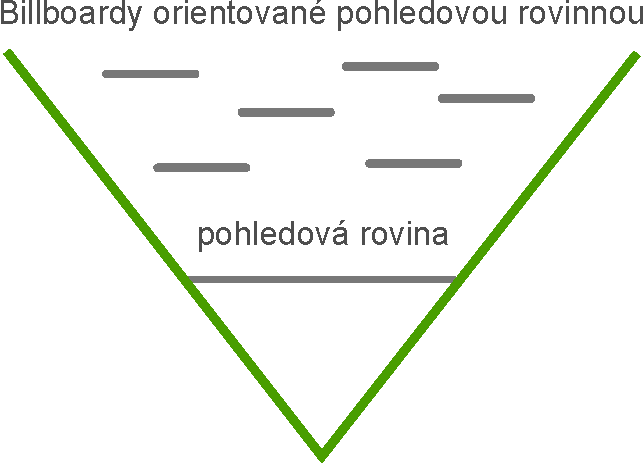
\includegraphics[width=0.5\textwidth]{obrazky-figures/viewplanealigned.pdf}
	\caption{Znázornění kamerou orientovaného billboardu. Inspirováno obrázkem z~knihy \emph{Real-Time Rendering Fourth Edition} \cite[kapitola 13.6]{ller2018real}. }
	\label{fig:billboard_camera_aligned}
\end{figure}
\subsection{Impostor}
Billboard nazývaný impostor lze vytvořit vykreslením složitého objektu z~aktuálního úhlu pohledu do textury, která je posléze použita jako textura tohoto billboardu. Okolí objektu na textuře musí být průhledné, aby nedošlo k~porušení iluze při pohybu kamery. Tato technika je vhodná pro vzdálené objekty, jelikož větší rotace billboardu je příliš patrná a je tak nutné objekt opět vykreslit. Příklad použití této techniky lze nalézt na obrázku \ref{fig:billboard_impostor_expample}.
\begin{figure}[h]
	\centering
	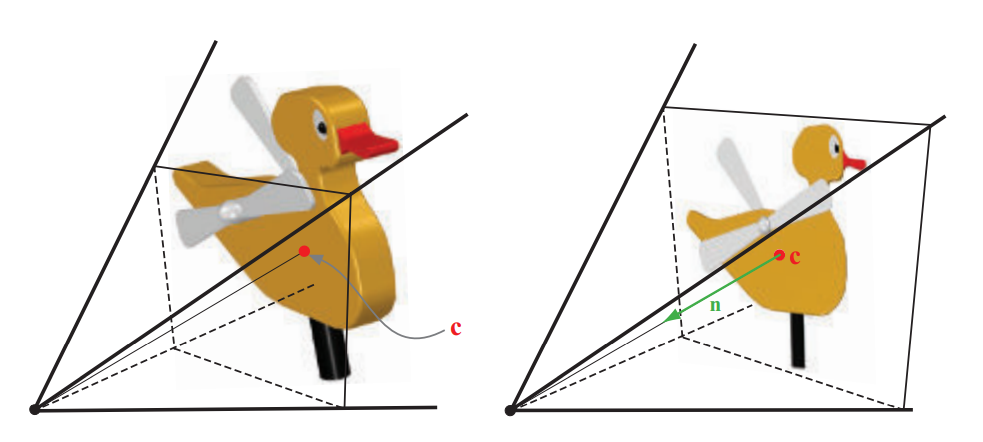
\includegraphics[width=1.0\textwidth]{obrazky-figures/test5.png}
	\caption{Příklad použití billboardu nazývaného impostor. Na levém obrázku se nachází 3D objekt, kde kamera směřuje na bod \(c\). Na pravém obrázku je objekt zobrazen pomocí vytvořené textury. Normála \(n\) směřuje od bodu \(c\) přímo na pozici kamery. Převzato z~knihy \emph{Real-Time Rendering Fourth Edition} \cite[kapitola 13.6]{ller2018real}. }
	\label{fig:billboard_impostor_expample}
\end{figure}
\subsection{Řazení podle průhlednosti}
Billboardy jsou ve většině případů zcela či částečně průhledné. Průhlednosti lze dosáhnout pomocí alpha blendingu. Avšak může vzniknout situace, kdy není průhlednost korektní, jako napřílad na obrázku \ref{fig:incorrect_order_blending}. To je způsobeno odstraňováním nepotřebných fragmentů při depth testu. Tento problém lze řešit řazením průhledných objektů, jak je popsáno v~knize \emph{Learn OpenGL} \cite{de2020learn}. Nejdříve se musí vykreslit neprůhledné objekty. Poté se průhledné objekty seřadí podle vzdálenosti od kamery a nakonec se vykreslí. 


Existují metody renderování průhledných objektů bez nutnosti předchozího řazení. Například metoda depth peeling využívá většího počtu z-bufferů a několika průchodů a je popsána v~knize \emph{Real-Time Rendering Fourth Edition} \cite[kapitola 5.5.1]{ller2018real}. Tyto metody jsou obvykle náročné na výkon grafické karty.  

\begin{figure}[H]
	\centering
	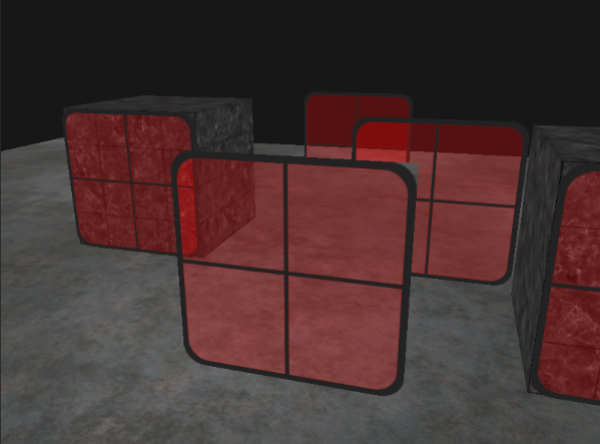
\includegraphics[width=0.5\textwidth]{obrazky-figures/blending_incorrect_order.png}
	\caption{Částečně průhledné objekty, vykreslené pomocí alpha blendingu bez použití řazení podle vzdálenosti od kamery, či jiné metody. Částečně průhledný objekt v~popředí tak zakrývá objekt za ním, který by měl být viditelný. Převzato z~knihy \emph{Learn OpenGL}\cite{de2020learn} }
	\label{fig:incorrect_order_blending}
\end{figure}
\section{Částicový systém}
Efekty jako například oheň, oblaka, mlha nebo tekutiny je náročné vykreslovat konvenčními metodami (jako objekty). Tyto objekty totiž nemají jasně definované povrchy, které by bylo možné snadno vykreslit. Některé se neustále transformují jen v~závislosti na čase nebo mohou i reagovat na prostředí. 

Pro zobrazení takových objektů navrhují autoři práce \emph{Particle systems—a technique for modeling a class of fuzzy objects} \cite{reeves1983particle} využít částicový systém\footnote{někdy také nazýván jako částicový emitor nebo částicový generátor}. Jedná se o~objekt v~prostoru, který však není zobrazen jako povrch tvořený primitivy, ale jako velké množství jednotlivých částic ovládaných částicovým systémem. Příklad použití částicového systému pro zobrazení komplexního efektu lze nalézt na obrázku \ref{fig:particles_expample}.

Částicový systém není statický, ale mění se v~závislosti na čase. Jednotlivé částice jsou generovány a zanikají, pohybují se v~prostoru a mohou měnit svůj vzhled. Částicový systém  podle autorů článku není deterministický, jelikož efekt, který má reprezentovat v~kontextu zobrazení v~počítačové grafice, také není. Některé vlastnosti částic jsou proto určovány stochastickými metodami. 

Činnost částicového systému v~každé iteraci renderovací smyčky je rozdělena na několik částí. Nejdříve musí vygenerovat nové částice a přidat je do systému. Těmto novým částicím musí přidělit počáteční vlastnosti. Ostatní částice, které nebyly v~této iteraci vytvořeny, jsou zkontrolovány, zda jejich doba života není rovna nule. Pokud ano, je částice zničena. Vlastnosti zbylých částic jsou aktualizovány. Nakonec jsou částice vykresleny. 
\begin{figure}[H]
	\centering
	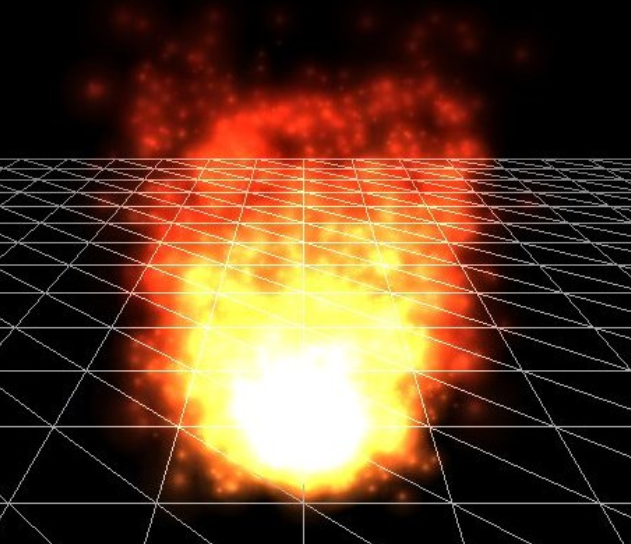
\includegraphics[width=0.5\textwidth]{obrazky-figures/test7.png}
	\caption{Zobrazení efektu ohně pomocí částicového systému. Převzato z~knihy \emph{Learn OpenGL} \cite[kapitola 56]{de2020learn}. }
	\label{fig:particles_expample}
\end{figure}

\subsection{Částice}
Částice je jednoduchý objekt v~prostoru, který je součástí částicového systému. Vzhledem k~jejich velkému počtu je nutné je zobrazovat co nejefektivněji, například jako billboardy. Je možné je zobrazovat i jako komplexní 3D objekty, může to však mít výrazné negativní efekty na výkon. 

\subsubsection{Vlastnosti částic}
Každá částice má obvykle několik základních vlastností, které určují její chování v~prostoru a vzhled. Každá vlastnost může být aktualizována v~každé iteraci renderovací smyčky. Jakým způsobem je aktualizována určuje chování celého systému a závisí na požadovaném efektu. Je například možné postupně snižovat průhlednost částice v~závislosti na vzdálenosti od pozice celého systému a vytvořit tak vizuální efekt postupného vyhasínání. Tento efekt je například patrný v~částicovém systému na obrázku \ref{fig:particles_expample}. 

\subsubsection*{Pozice} Někdy také \emph{posun}. Je to vektor, který určuje, kde se částice nachází relativně k~pozici celého systému. Počáteční pozice je určena náhodným výběrem z~oblasti, která je definována \emph{tvarem emitoru}. Tento tvar může být například koule (oblast je definována poloměrem \(R\)), kvádr (omezené souřadnice \(x y z\)) nebo libovolný dvourozměrný tvar. Emitory různých tvarů jsou vyobrazeny na obrázku \ref{fig:particles_position_expample}. Pozice částic je obvykle relativní ke středu tvaru emitoru. Samotný střed využívá stejného světového souřadnicového systému jako ostatní objekty.
\begin{figure}[H]
	\centering
	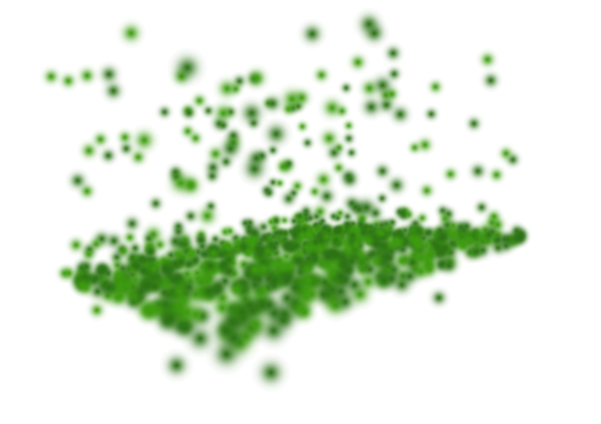
\includegraphics[width=0.24\textwidth]{obrazky-figures/rectangle_particles.png}
	
\includegraphics[width=0.24\textwidth]{obrazky-figures/circle_particles.png}
	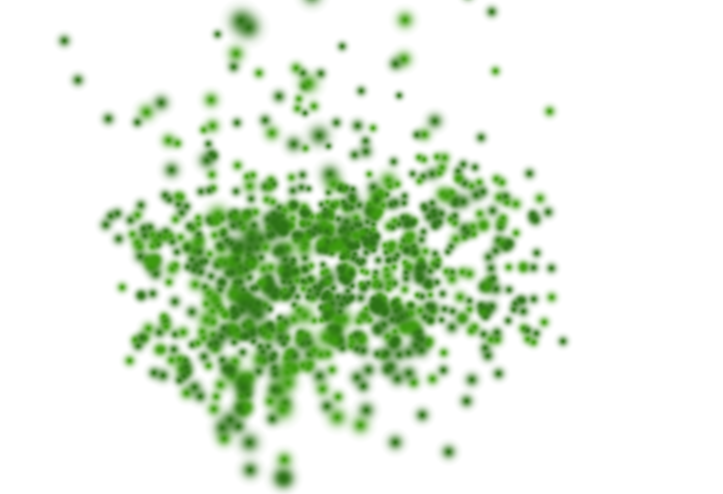
\includegraphics[width=0.24\textwidth]{obrazky-figures/square_particles.png}
	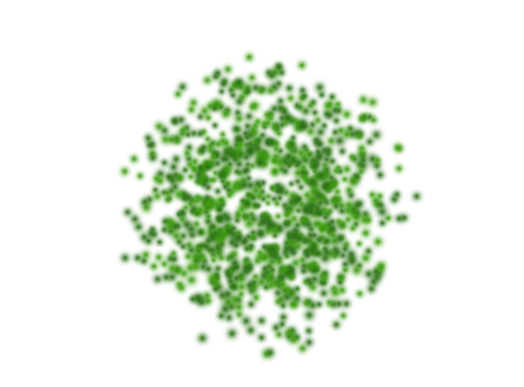
\includegraphics[width=0.24\textwidth]{obrazky-figures/sfere_particles.png}
	\caption{Různé tvary emitoru částicového systému. Na prvním obrázku má částicový systém tvar obdelníku. Na dalším je tento tvar kruh, na předposledním krychle a na posledním je ve tvaru koule. K~vytvoření těchto částicových efektů byl použit herní engine \emph{Unity} od společnosti \emph{ Unity Technologies}. }
	\label{fig:particles_position_expample}
\end{figure}
\subsubsection*{Rychlost} Rychlost může být konstantní, nebo se v~čase měnit (například akcelerovat). Počáteční rychlost \(S_i\) je určena vztahem popsaným rovnicí \ref{eq:4}.
\begin{equation}
S_i = S_m + Rand() \cdot S_v
\label{eq:4}
\end{equation}
\(S_m\) je průměrná rychlost částice. K~ní je přičtena náhodná hodnota \(Rand()\) vynásobená rozsahem rychlosti \(S_v\). 
\subsubsection*{Směrový vektor} Určuje, kterým směrem se má částice v~prostoru pohybovat. Mění se podle \emph{generačního tvaru}. Pokud je jím sféra, tak bude směřovat směrem od středu této sféry. V~případě kruhu a obdélníku by měl směřovat přímo vzhůru. Směr je ještě možné upravit rotací náhodně zvoleným úhlem. Směr se v~průběhu života částice může měnit, například vlivem gravitace nebo vlivem prostředí (kolize).

Pro reálnější simulaci částic je možné spojit směr a rychlost do jednoho vektoru a přidat atributy jako akcelerace, hmotnost a podobné fyzikální veličiny. Tato a další rozšíření navrhuje a zkoumá autor práce \emph{Particle system dynamics} \cite{witkin1999particle}. 

\subsubsection*{Barva a textura} Počáteční barva může být vždy stejná, nebo náhodně určená (například ohňostroj zobrazený na obrázku \ref{fig:particles_color_expample}). Také se může měnit podle ostatních vlastností částice (rychlost, pozice). Částice může mít také texturu a normálovou mapu. Je tak možné na částice aplikovat světlo. Textura i barva mohou být částečně, či zcela průhledné. V~3D prostoru je v~takovém případě nutné vyřešit problematiku řazení podle průhlednosti.

\begin{figure}[H]
	\centering
	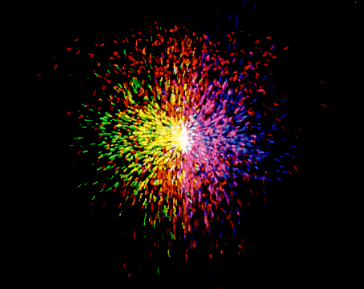
\includegraphics[width=0.5\textwidth]{obrazky-figures/particles_old.png}
	\caption{Příklad částic ohňostroje, kde jednotlivé částice mají náhodnou barvu. Převzato z~práce \emph{Particle systems, technique for modeling a class of fuzzy objects} \cite{reeves1983particle}. Tento částicový efekty byl vytvořen jako součást práce, a to již v~roce 1983. Autoři práce také zmiňují aplikací podobných efektů v~ranných počátcích počítačové grafiky v~kinematografii, například ve filmu \emph{Return of the Jedi}.  }
	\label{fig:particles_color_expample}
\end{figure}

\subsubsection*{Doba života} Hodnota, která určuje, za jak dlouho bude částice smazána. Při každé aktualizaci se tato hodnota sníží a pokud dosáhne hodnoty nula, tak je částice ze systému odstraněna. Počáteční doba života může být pro všechny částice konstantní, nebo určená náhodně. Částicový systém také může při splnění určité podmínky rovnou nastavit dobu života částice na 0, a tím ji odstranit. Takovou podmínkou je například opuštění určitého prostoru.

\subsection{Generování}
Počet částic v~systému ovlivňuje jeho celkový vzhled. Existuje několik způsobů, jak částice generovat. 

V~knize \emph{Learn OpenGL} \cite{de2020learn} je popsána metoda, ve které je nutné vygenerovat \(n\) částic a poté každou částici, která zemře následkem klesnutí doby života na hodnotu nula, vyresetovat. Zajistí se tak konstatní počet částic v~systému, což může mít pozitivní efekt na výkonnostní nároky celého systému. Není totiž třeba alokovat žádnou další paměť.

Další metodou, popsanou v~původní práci \cite{reeves1983particle}, je generovat částice pomocí kontrolované stochastické metody. Počet částic v~systému \(P_n\) je tak určen podle rovnice \ref{eq:5}.
\begin{equation}
P_n = P_m + Rand() \cdot P_v
\label{eq:5}
\end{equation}
\(P_m\) je požadovaný průměrný počet částic v~systému. \(Rand()\) je náhodná hodnota v~rozsahu od \(-1.0\) do \(+1.0\) a hodnota \(P_v\) je rozsah maximální odchylky od průměru. 

Tento vztah je možné modifikovat, například přidáním požadovaného obsahu systému na obrazovce \(P_o\) podle rovnice \ref{eq:6} a dosáhnout tak zvýšení detailu systému při bližším pohledu. 
\begin{equation}
P_n = (P_m + Rand() \cdot P_v) \cdot P_o
\label{eq:6}
\end{equation}
Dále je možné modifikovat hodnotu průměrného počtu částic \(P_m\). Dojde tak k~postupnému snižování či zvyšování počtu částic v~systému, a způsobit tak například efekt vyhasínání.


\section{Light Field}
Zobrazení 3D scén je standardně uskutečňováno pomocí geometrických tvarů, materiálů a světel. \emph{Image-based rendering} je alternativní metoda, kde se k~zobrazování využívá předem vytvořených snímků. Zobrazování pomocí této metody je obvykle výkonnostně nenáročné a použité snímky mohou být libovolně kvalitní (například snímky reálného světa). 

V~práci \emph{Light Field Rendering} \cite{levoy1996light} autoři navrhují metodu zobrazování 3D scény pomocí zachycení a následné reprodukce \emph{light fieldu}. Light field reprezentuje světelné paprsky, které snímaný objekt vyzáří nebo odrazí. Je možné je zachytit, uložit a poté reprodukovat. Hlavní výhodou zobrazování pomocí light fieldu oproti jiným metodám image-based renderingu je schopnost zobrazovat původní scénu z~libovolného úhlu pohledu, ze kterého byl zachycen. 

Existuje více způsobů, jak zachycené světlo parametrizovat.  V~originální práci autoři navrhují reprezentaci pomocí 4D funkce, kde je každý paprsek světla brán jako přímka protínající dvě roviny. Jednotlivé parametry této funkce jsou souřadnice průsečíků přímky a těchto rovin. Souřadnicový systém na první rovině je \((u,v)\) a na druhé \((s,t)\). Oba souřadnicové systémy jsou omezeny na interval 0 až 1. Výsledná funkce
\[L(u,v,s,t)\]
tedy reprezentuje každý světelný paprsek vyzářený snímanou scénou, jak je znázorněno na obrázku \ref{fig:lightfield_coordinates}. 

\begin{figure}[h]
	\centering
	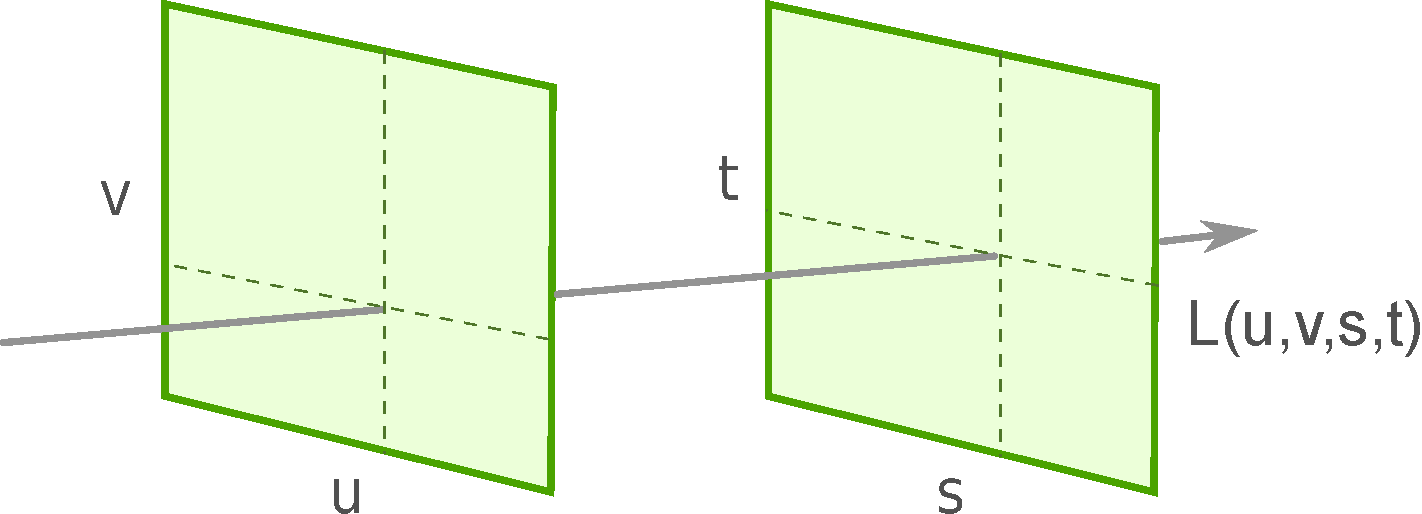
\includegraphics[width=0.8\textwidth]{obrazky-figures/lightfield_eq.pdf}
	\caption{Znázornění světelného paprsku protínající roviny \((u,v)\) a \((s,t)\). Inspirováno obrázkem z~původní práce \emph{Light Field Rendering} \cite{levoy1996light}. }
	\label{fig:lightfield_coordinates}
\end{figure}

Velmi podobná parametrizace světla je zkoumána i v~práci \emph{The Lumigraph} \cite{gortler1996lumigraph}. 4D lumigraph také parametrizuje světelné paprsky pomocí jejich průsečíků se dvěma rovinami. Celý lumigraph se skládá z~šesti páru takových rovin souběžných z~různými osami. 

Další způsob parametrizace zachyceného světla je plenoptická funkce, kterou navrhli autoři práce \emph{The Plenoptic Function and
the Elements of Early Vision} \cite{bergen1991plenoptic}. Tato funkce obsahuje sférické souřadnice, vlnovou délku, čas a souřadnice kamery. Sférické souřadnice je také možné nahradit za souřadnice $(x,y)$ nacházející se na rovině. Light field vychází právě z~plenoptické funkce a je její omezenou variantou.


\subsection{Tvorba a reprezentace}
\label{sec:theory_create}
Light fieldy mohou být virtuální nebo reálné. Virtuální jsou vytvořeny z~renderované scény a reálné zachycením fyzických světelných paprsků.

Virtuální light field je vytvářen zachycením 2D pole obrázků. Jednotlivé obrázky reprezentují zachycené paprsky na rovině \((s,t)\) pro fixní pozici na rovině \((u,v)\). Tato reprezentace je vizualizována na obrázku \ref{fig:lightfield_reprezentation}. Alternativně lze light field ukládat s~opačnými souřadnicemi, kde každý obrázek reprezentuje průsečík s~rovinou \((u,v)\) pro fixní pozici průsečíku s~rovinou \((s,t)\). Virtuální light field reprezentovaný jednou z~těchto metod je však pouze nespojitou aproximací ideáního light fieldu.
\begin{figure}[h]
	\centering
	\includegraphics[width=1.0\textwidth]{obrazky-figures/lightfield_reprezentation-comp.pdf}
	\caption{Vizualizace jedné z~možných reprezentací light fieldu. Funkce je ve formě $L(u, v, s, t)$, každá souřadnice $uv$ tedy obsahuje množinu hodnot na různých $st$ souřadnicích. Autorem virtuálního light fieldu použitého pro vizualizaci je Gordon Wetzstein \cite{lightfieldarchive}  }
	\label{fig:lightfield_reprezentation}
\end{figure}

Reálné light fieldy lze zachytit různými způsoby. Jedna varianta je použít mřížku kamer a pořídit 2D pole fotografií, nebo kameru či objekt postupně posunovat. Existují také speciální kamery, které umožňují přímo zachytit fotografie v~podobě plenoptické funkce. Příklad takové kamery lze nalézt na obrázku \ref{fig:lytro}.


Výsledný light field může být velmi objemný. Díky velké redundaci dat lze však light field velmi efektivně komprimovat. V~originální práci \cite{levoy1996light} autoři navrhují způsob, jak data komprimovat s~efektivitou až 118:1. Srovnání kompresních metod light fieldu se například věnují autoři práce \emph{Comparison of light field compression methods} \cite{barina2021comparison}.

\begin{figure}[H]
	\centering
	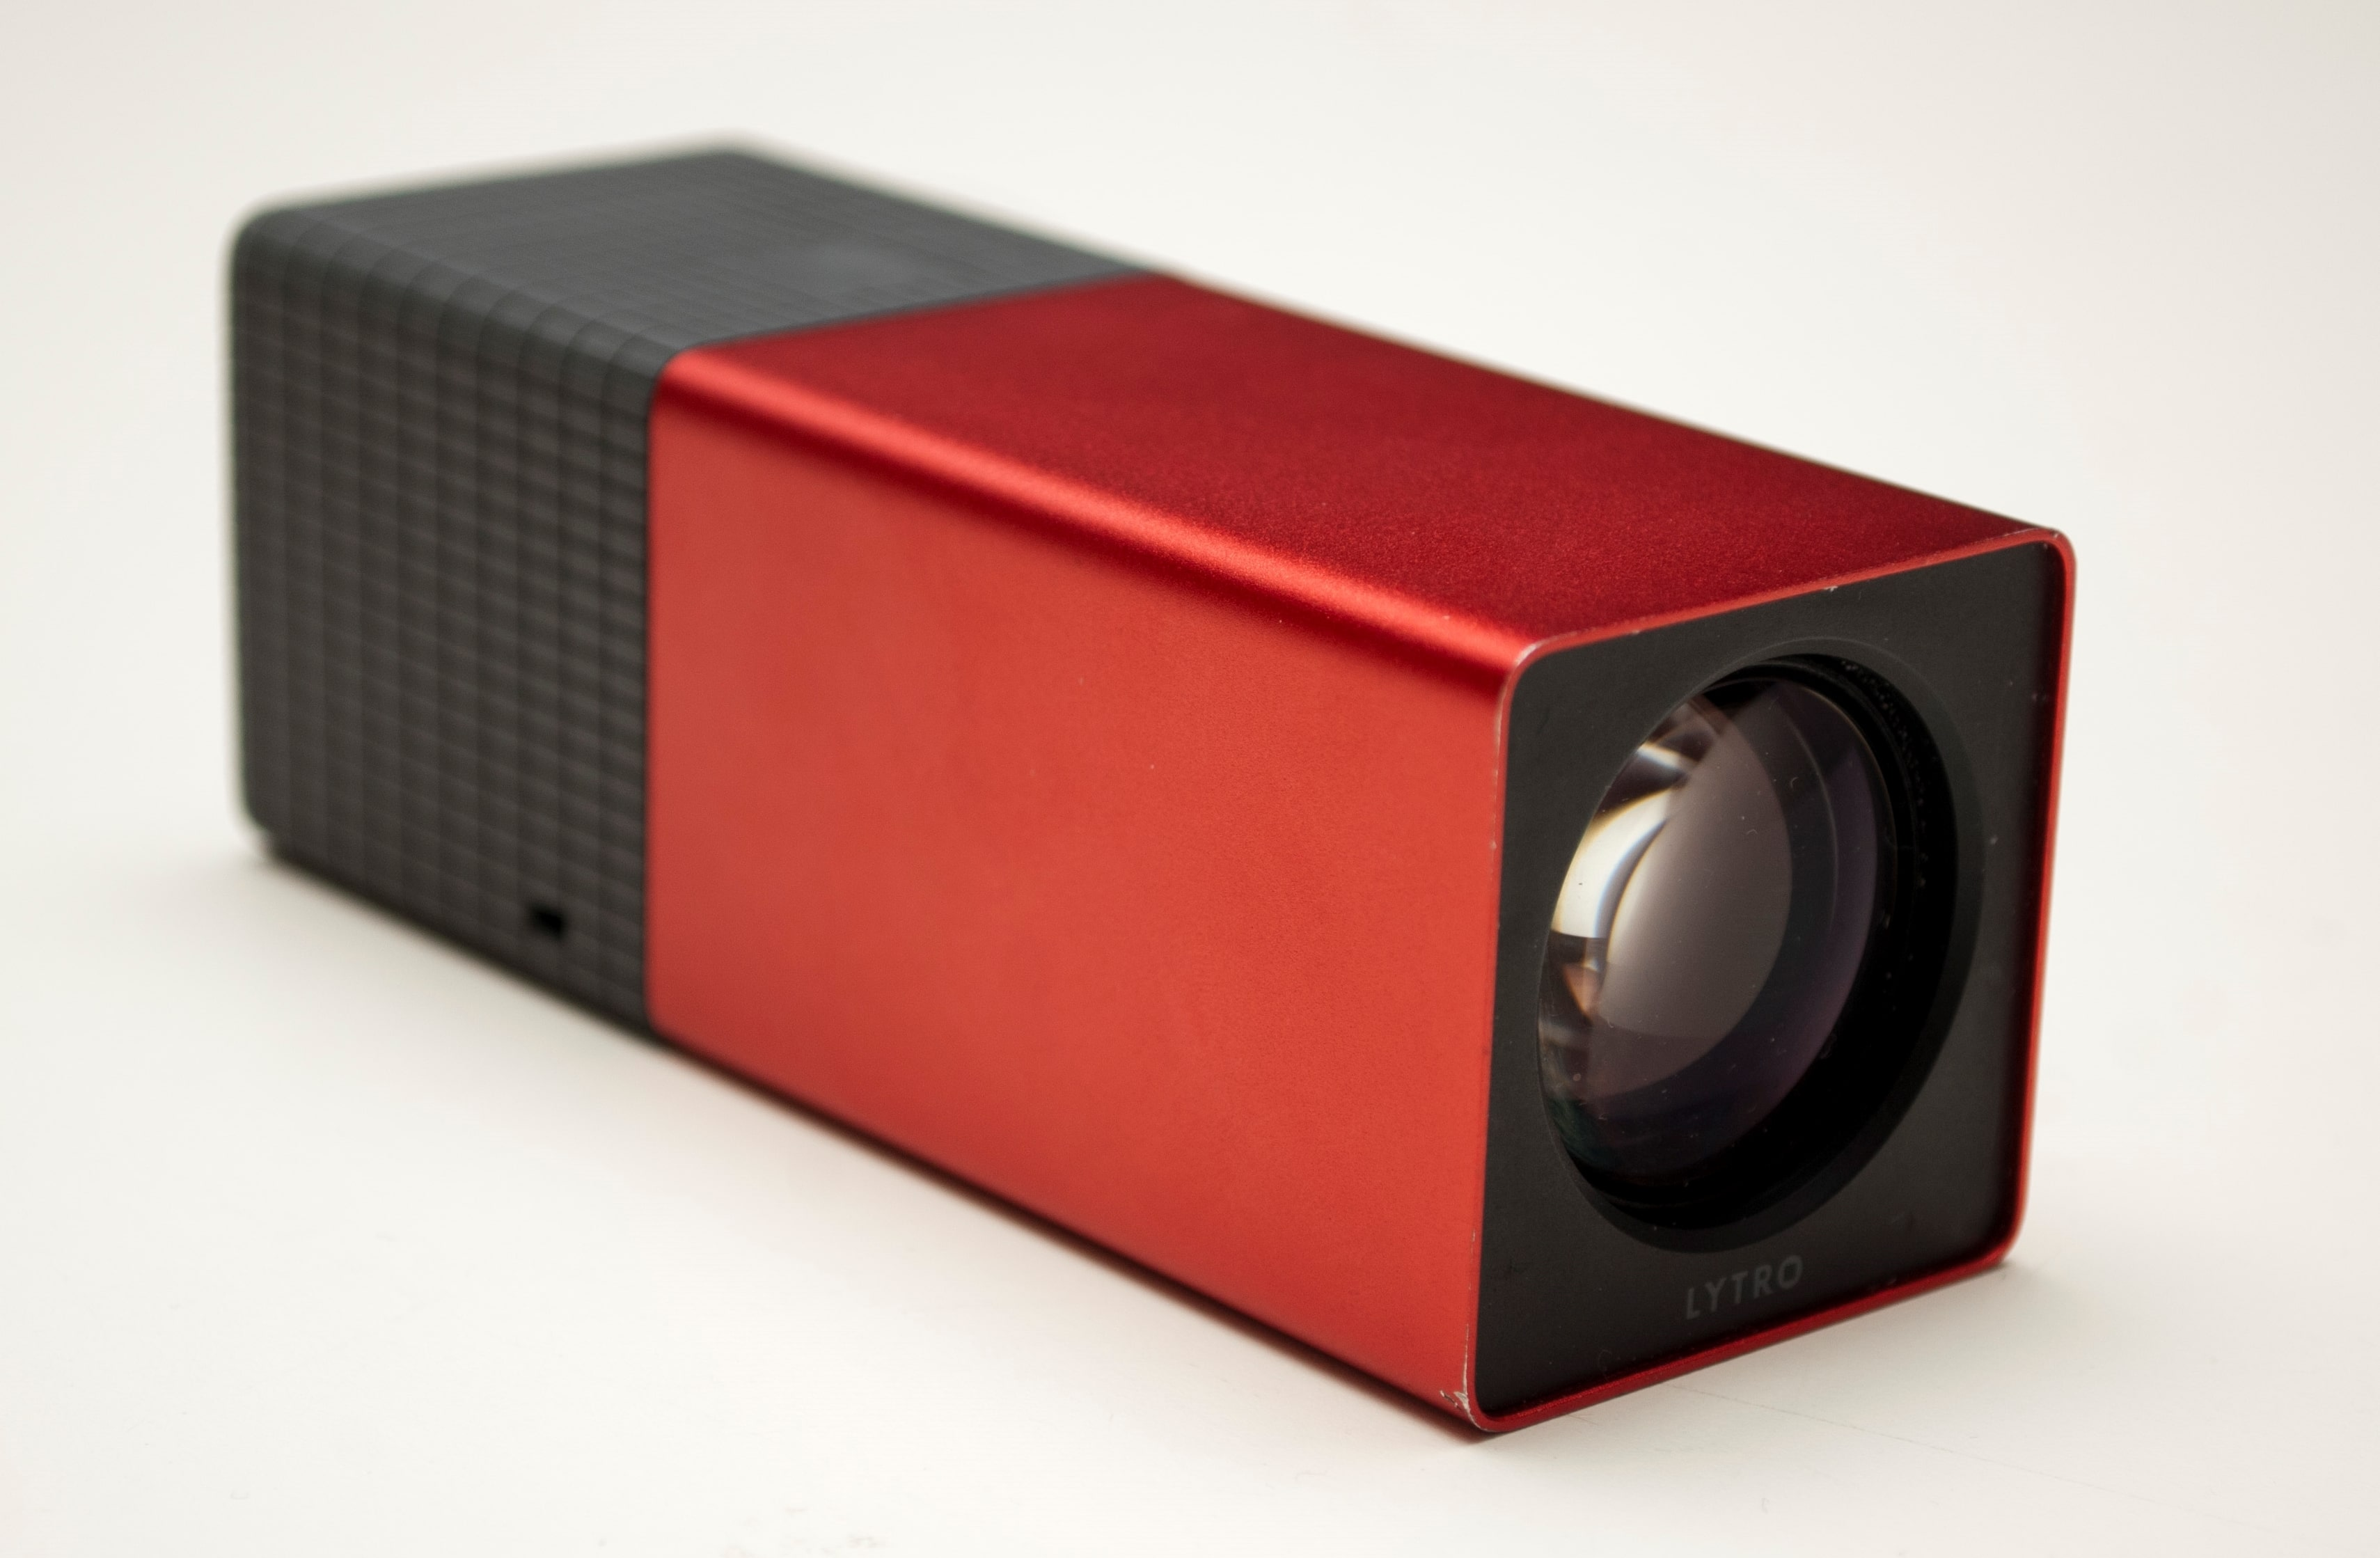
\includegraphics[width=0.49\textwidth]{obrazky-figures/lytro1-min.jpg}
	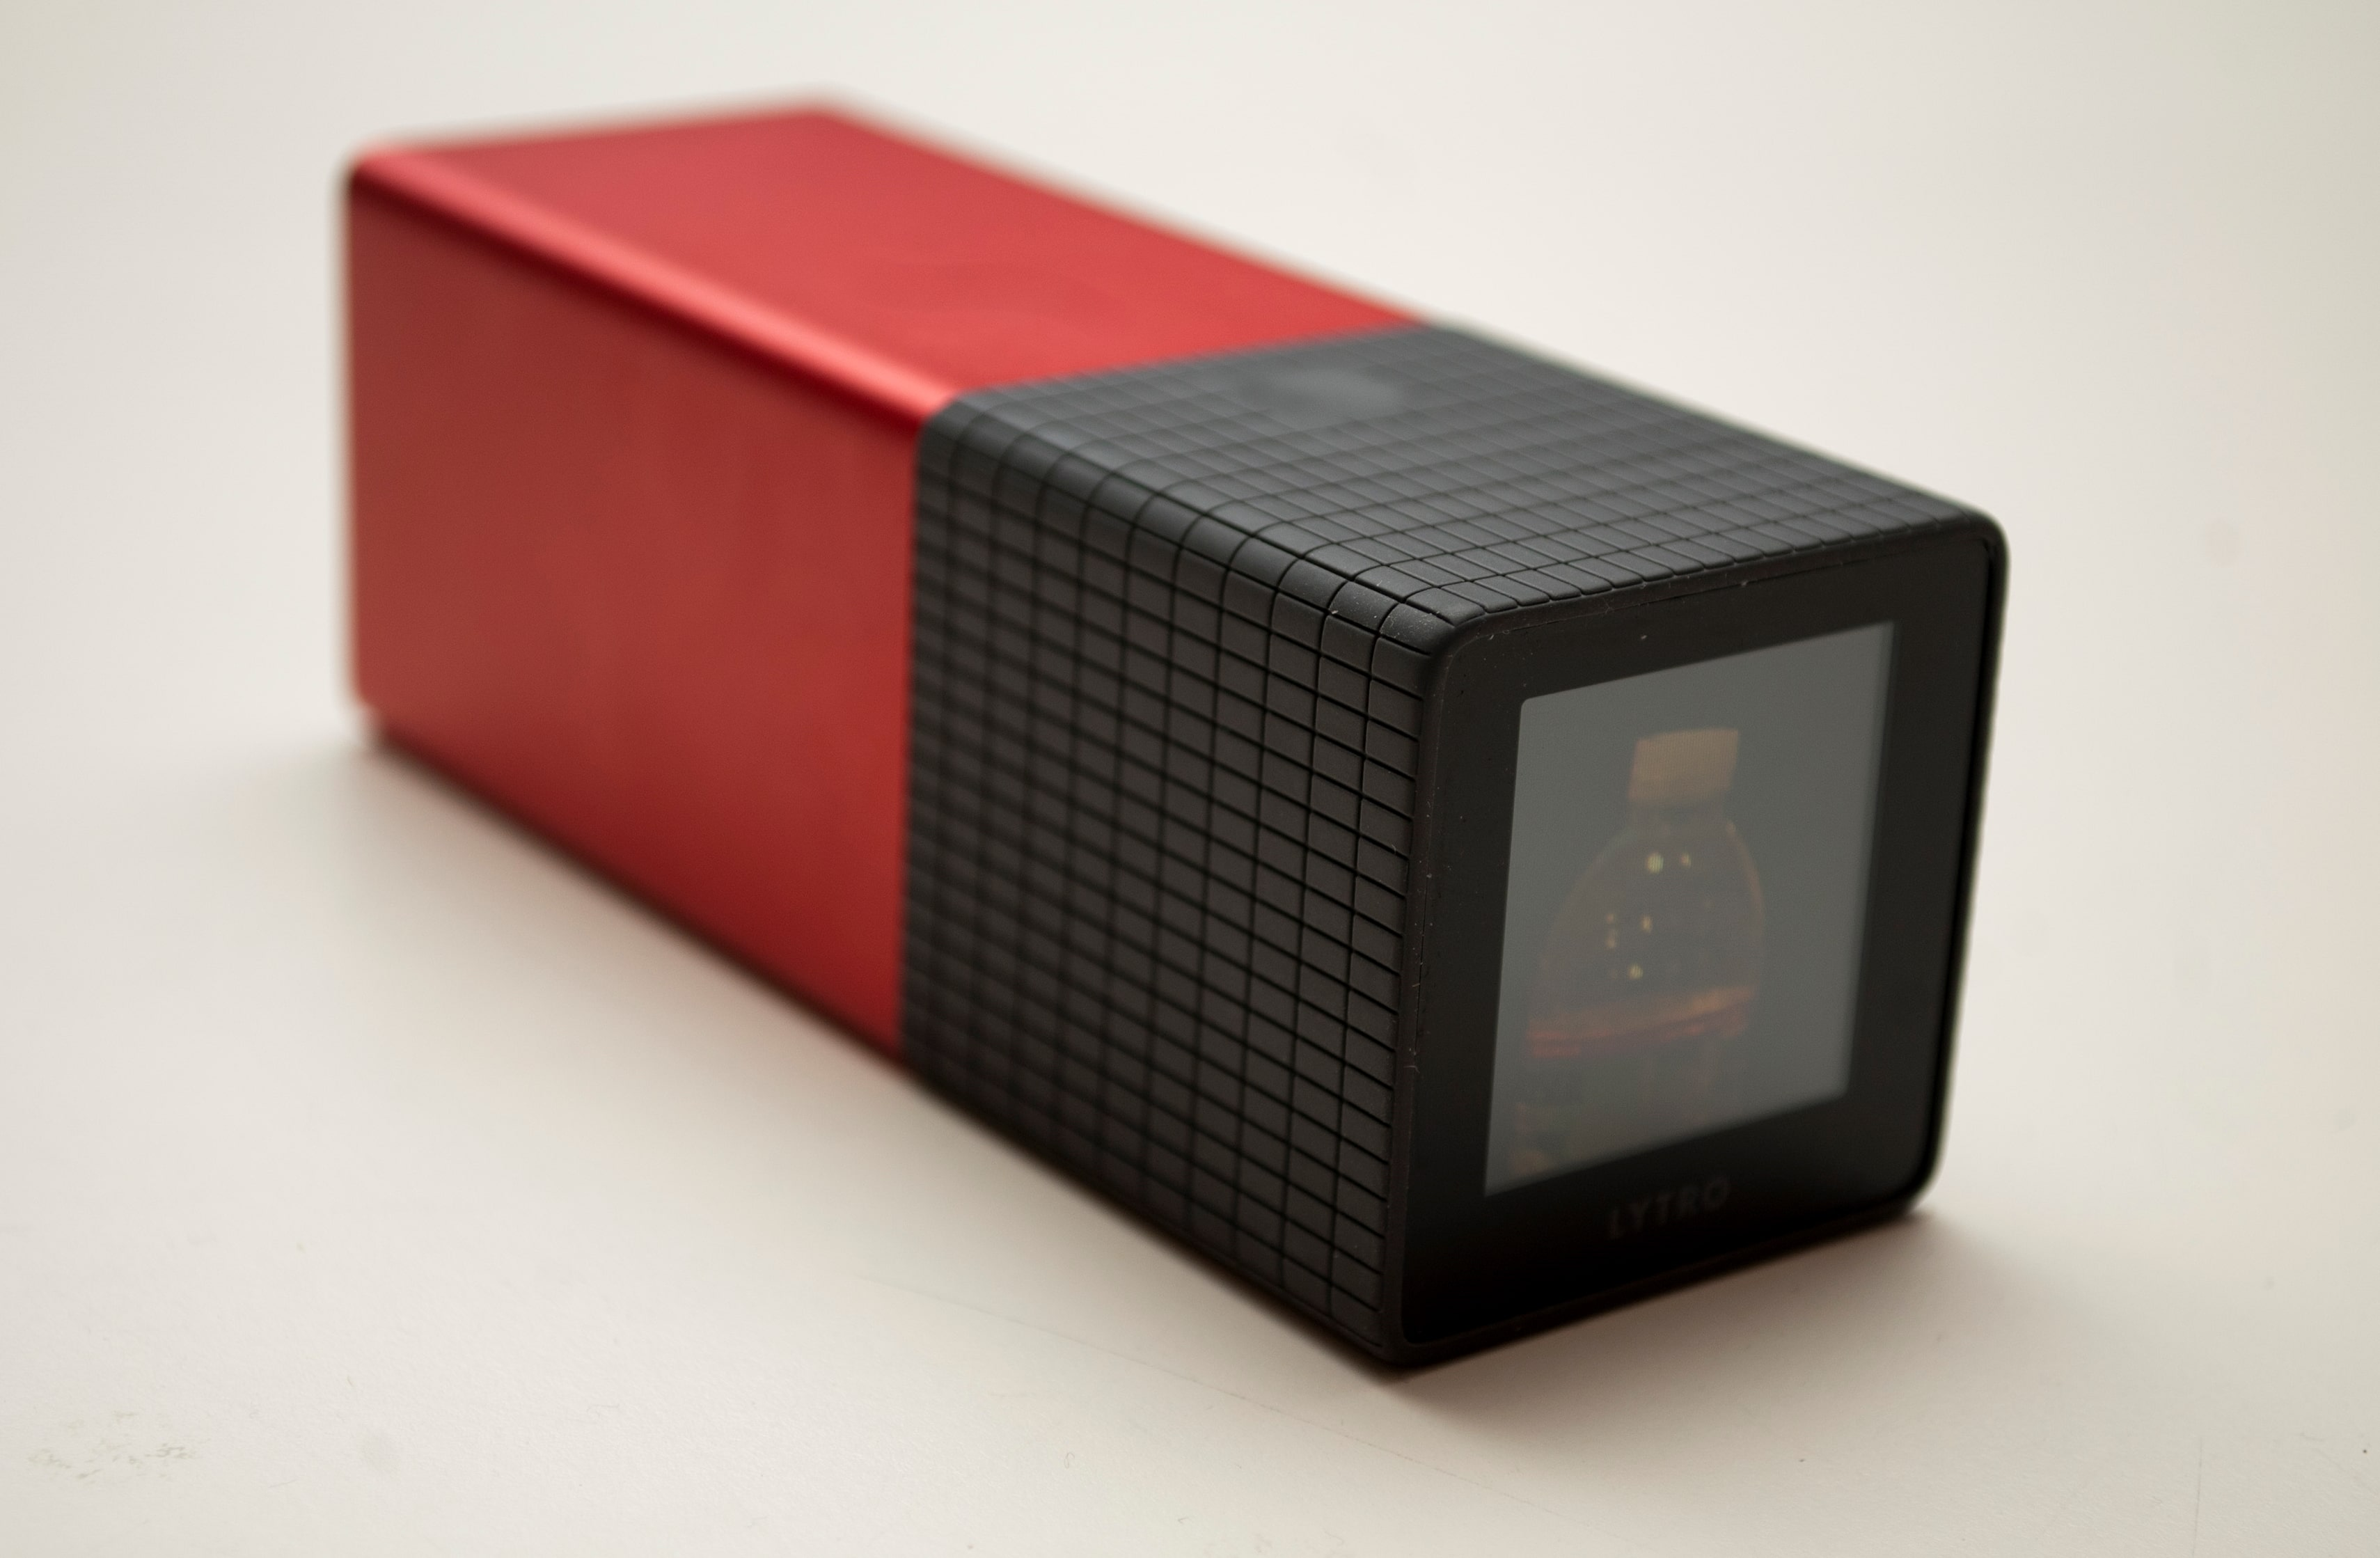
\includegraphics[width=0.49\textwidth]{obrazky-figures/lytro2-min.jpg}
	\caption[Caption for LOF]{Kamera od společnosti Lytro, Inc. umožňující zachytit fotografii jako plenotickou \footnotetext{bu} funkci. Fotoaparát je vybaven maticí čoček a speciálním senzorem určeným právě ke snímání light fieldu\protect\footnotemark. }
	\label{fig:lytro}
\end{figure}

\footnotetext{zdroj: https://www.digitaltrends.com}
\subsection{Zobrazování}
\label{sec:lightfield_zobrazeni}
Při zobrazování light fieldu je nutné sestavit 2D snímek ze 4D funkce reprezentující light field. Nejdříve je nutné spočítat souřadnice \((u,v,s,t)\) pro každý paprsek světla protínající kameru. Alternativně je také možné využít pohledové matice a texturového mapování pro určení \((u,v)\) souřadnic a následného mapování \((s,t)\) souřadnic na kameru. 

Při sestavování snímku je nutné vzorkovat původní light field. Při vzorkování se najdou nejbližší vzorky a výsledná hodnota vznikne pomocí jejich interpolace. Zvolená metoda interpolace má vliv na efektivitu a může způsobovat artefakty ve výsledném snímku. 

Nejjednodušší metoda je použití nejbližšího vzorku. Dle Nyquist–Shannon vzorkovacího theoremu\cite{por2019nyquist} lze tuto metodu použít pouze v~případě, že je vzorkovací frekvence alespoň dvakrát větší, než frekvence vzorku. Případný aliasing a vzniklé rozmazávání je možné řešit použitím konečné hloubky ostrosti \footnote{anglicky depth of field}, avšak je poté nutné zvolit vhodnou clonu. Pokud je počet vzorků nízký, je nutné použít lepší interpolaci. Lze použít lineární interpolaci aplikovanou pouze na \((u,v)\) souřadnice, nebo quadrilineární interpolaci nad souřadnicemi \((u,v,s,t)\). Poslední zmíněná metoda vytváří nejmenší počet vizuálních artefaktů, což je přínosné zejména pro pohybující se objekty. Je však výpočetně značně náročnější než metoda lineární interpolace. Na redukci aliasingu vykreslovaného light fieldu lze například použít mipmaping.


\section{Mipmapování}
Pixely textury obvykle neodpovídají pixelům povrchu, na který jsou nanášeny. Textura musí být zvětšována či zmenšována tak, aby pixely odpovídaly povrchu. Při zmenšení může být více pixelů mapováno na jedno místo, a je tak nutné použít \emph{minification filter}. Při zvětšení dochází k~opačnému jevu a je nutné zvolit \emph{magnification  filter}. Například v~knize \emph{Introduction to Computer Graphics} \cite{foley1994introduction} jsou popsány dva typy filtrování: pomocí nejbližšího pixelu textury a lineární. 

\pagebreak

Spolu s~filtrováním uvádějí autoři možnost použít \textbf{mipmapování}. Mipmapa je kolekce různých velikostí jedné textury. Při filtrování je pak možné vybrat pouze nejbližší velikost textury odpovídající povrchu. Tento přístup může velmi urychlit přístup k~textuře a zefektivnit cachování, jelikož je obvykle využívaná textura menší než textura originální. 

Autoři také uvádějí, že mipmapovaná textura je obvykle jen o~jednu třetinu objemnější než originální textura. Je však možné dosáhnout i paměťových úspor v~případě, že je do paměti nahrána pouze potřebná část mipmapové textury. 

Další významnou výhodou mipmapingu je redukce aliasingu. Tento efekt lze pozorovat například na obrázku \ref{fig:mipmap_alias}. Výraznou nevýhodou mipmapingu je nutnost mipmapovou texturu generovat. Je sice možné ji vygenerovat před začátkem vykreslování, ale je nutné ji generovat za běhu v~případě, že se textura mění. 

\begin{figure}[H]
	\centering
		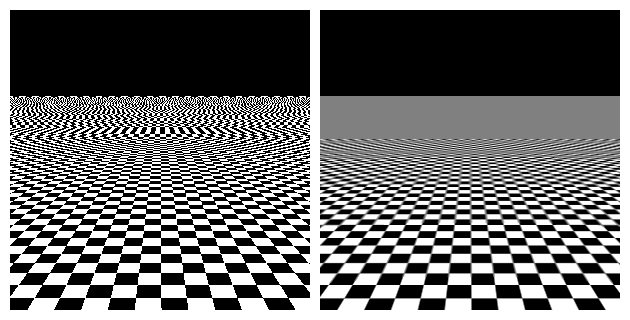
\includegraphics[width=1.0\textwidth]{obrazky-figures/mipmap1.png}
	\caption{Příklad redukce aliasingu s~pomocí mipmapování. Na levém obrázku se nachází textura šachovnice bez použití mipmapování. Na pravém obrázku se nachází stejná textura, avšak s~využitím mipmapování \protect\footnotemark.}
	\label{fig:mipmap_alias}
\end{figure}
\footnotetext{zdroj obrázku: https://textureingraphics.wordpress.com}

\chapter{Návrh}
Tato kapitola se věnuje návrhu architektury a metodice testování vytvořeného nástroje. Je v~ní podrobně popsáno, jak byla navrhnuta metoda kombinace light fieldu a částicových efektů. Také jsou v~kapitole popsány části, ze který se architektura aplikace skládá.

Cílem výsledné aplikace je vykreslovat částicový systém, kde jsou jednotlivé částice billboardy a jejich textura je tvořena pomocí light fieldu. Light field textura je tvořena dynamicky za běhu vykreslováním 3D objektu pod potřebnými úhly. Tento proces je znázorněn na obrázku \ref{fig:navrh_bp}. Částice také mohou používat větší množství těchto textur. Dalším cílem je, aby aplikace obsahovala možnost přepínat mezi několika scénami, které demonstrují různou funkcionalitu.

\begin{figure}[H]
	\centering
		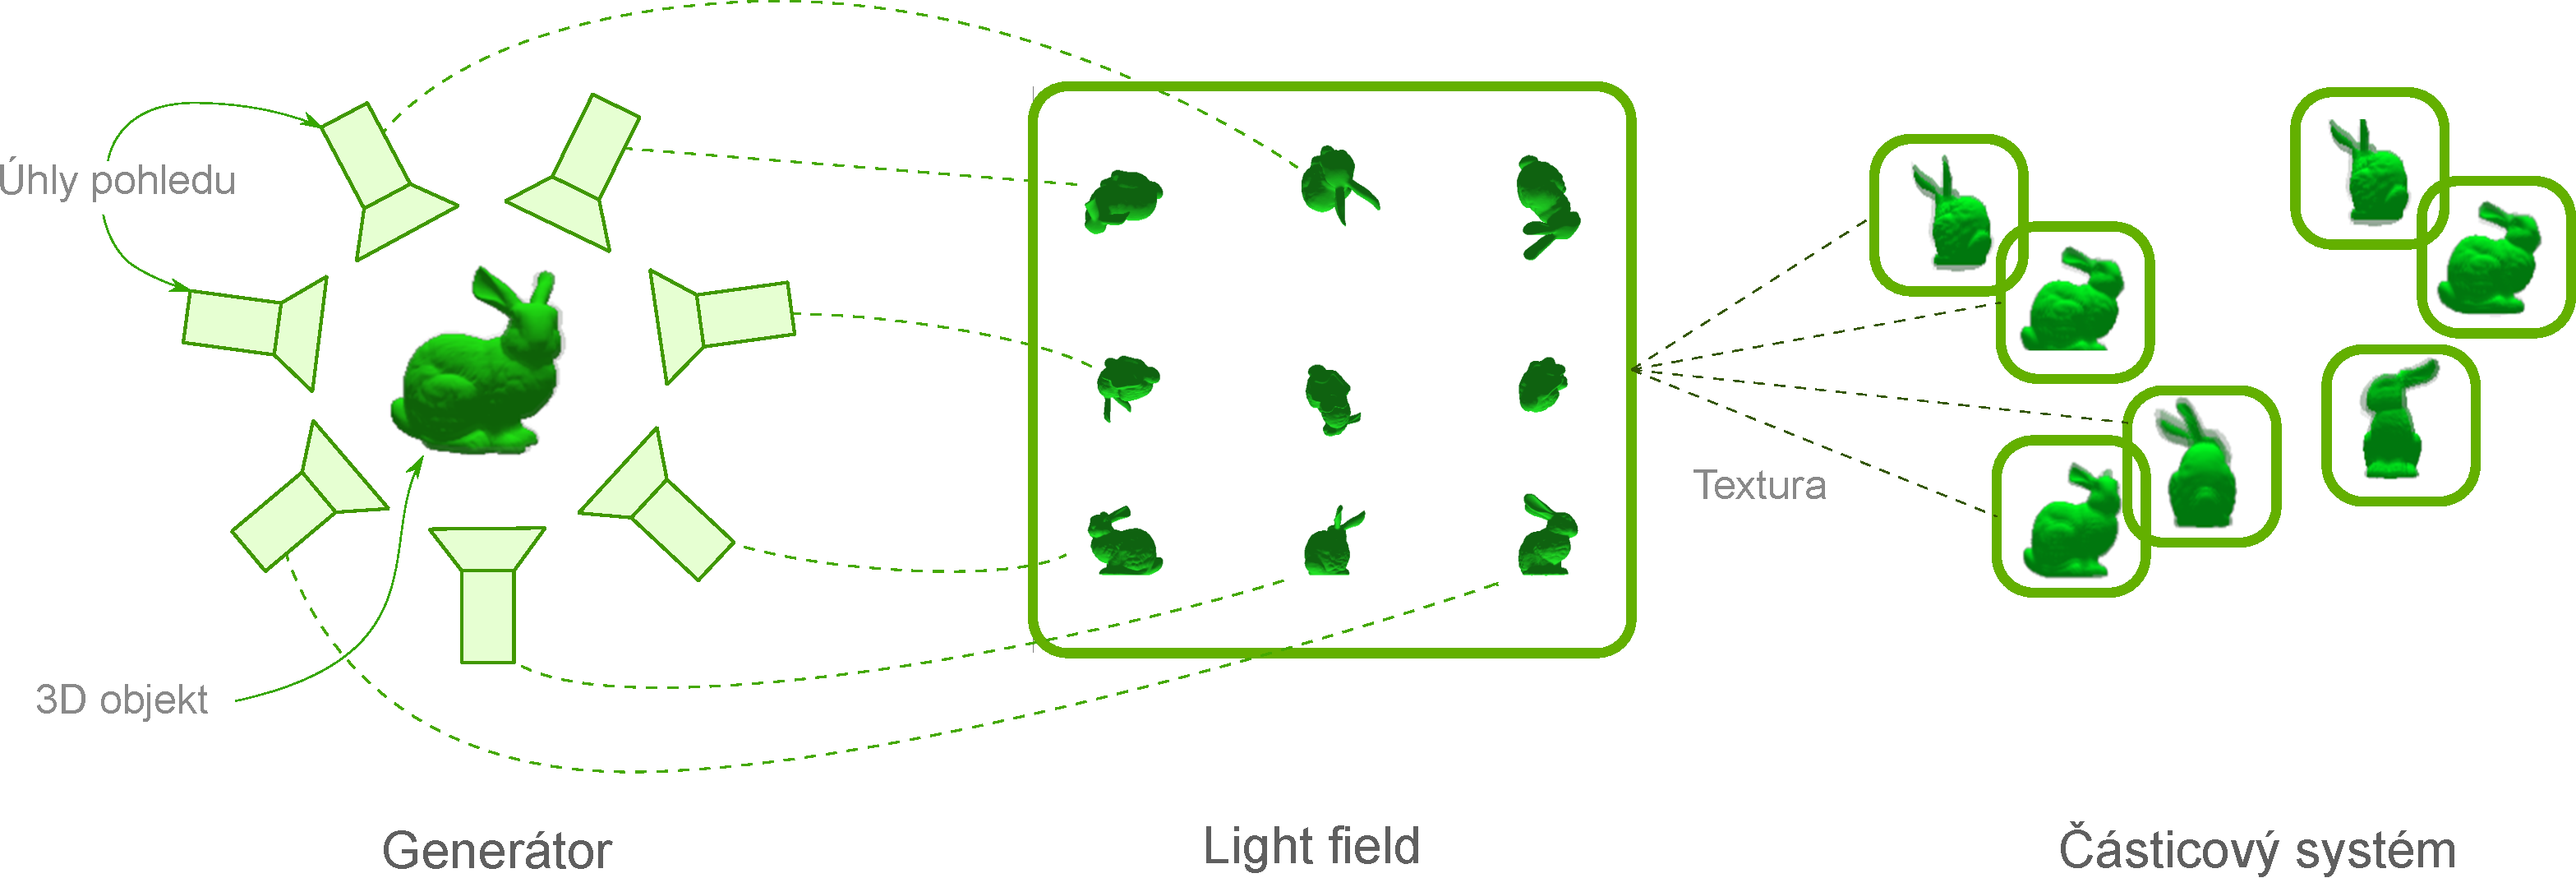
\includegraphics[width=1.0\textwidth]{obrazky-figures/bpnavrh.pdf}
	\caption{Jednotlivé moduly nástroje a vztahy mezi nimi.}
	\label{fig:navrh_bp}
\end{figure}

Nástroj je rozdělen na několik modulů, které mohou být použity i samostatně. Uživatelské rozhraní umožňuje změnu různých parametrů systému a přepínání \emph{scén}. Každá scéna obsahuje jiný částicový systém. Při změně scény se vytvoří \texttt{model} obsahující objekt a je předán modulu \texttt{generátor}. Hlavním účelem generátoru je generování light field dat. Generátorů může existovat větší množství a všechny jsou uskladněny v~jednom objektu \texttt{store}, který je předává modulu \texttt{částicový systém}. Hlavním údělem tohoto modulu je vykreslování částic. Dále také vytváří \texttt{tabulku potřebných úhlů pohledu}, pomocí které mohou generátory dovytvářet potřebná data light fieldu. Součástí částicového systému je také \texttt{simulátor}, který zajištuje správu a simulaci částic. Jednotlivé moduly a vztahy mezi nimi jsou znázorněny na Obrázku \ref{fig:navrh_uml}.

\begin{figure}[H]
	\centering
		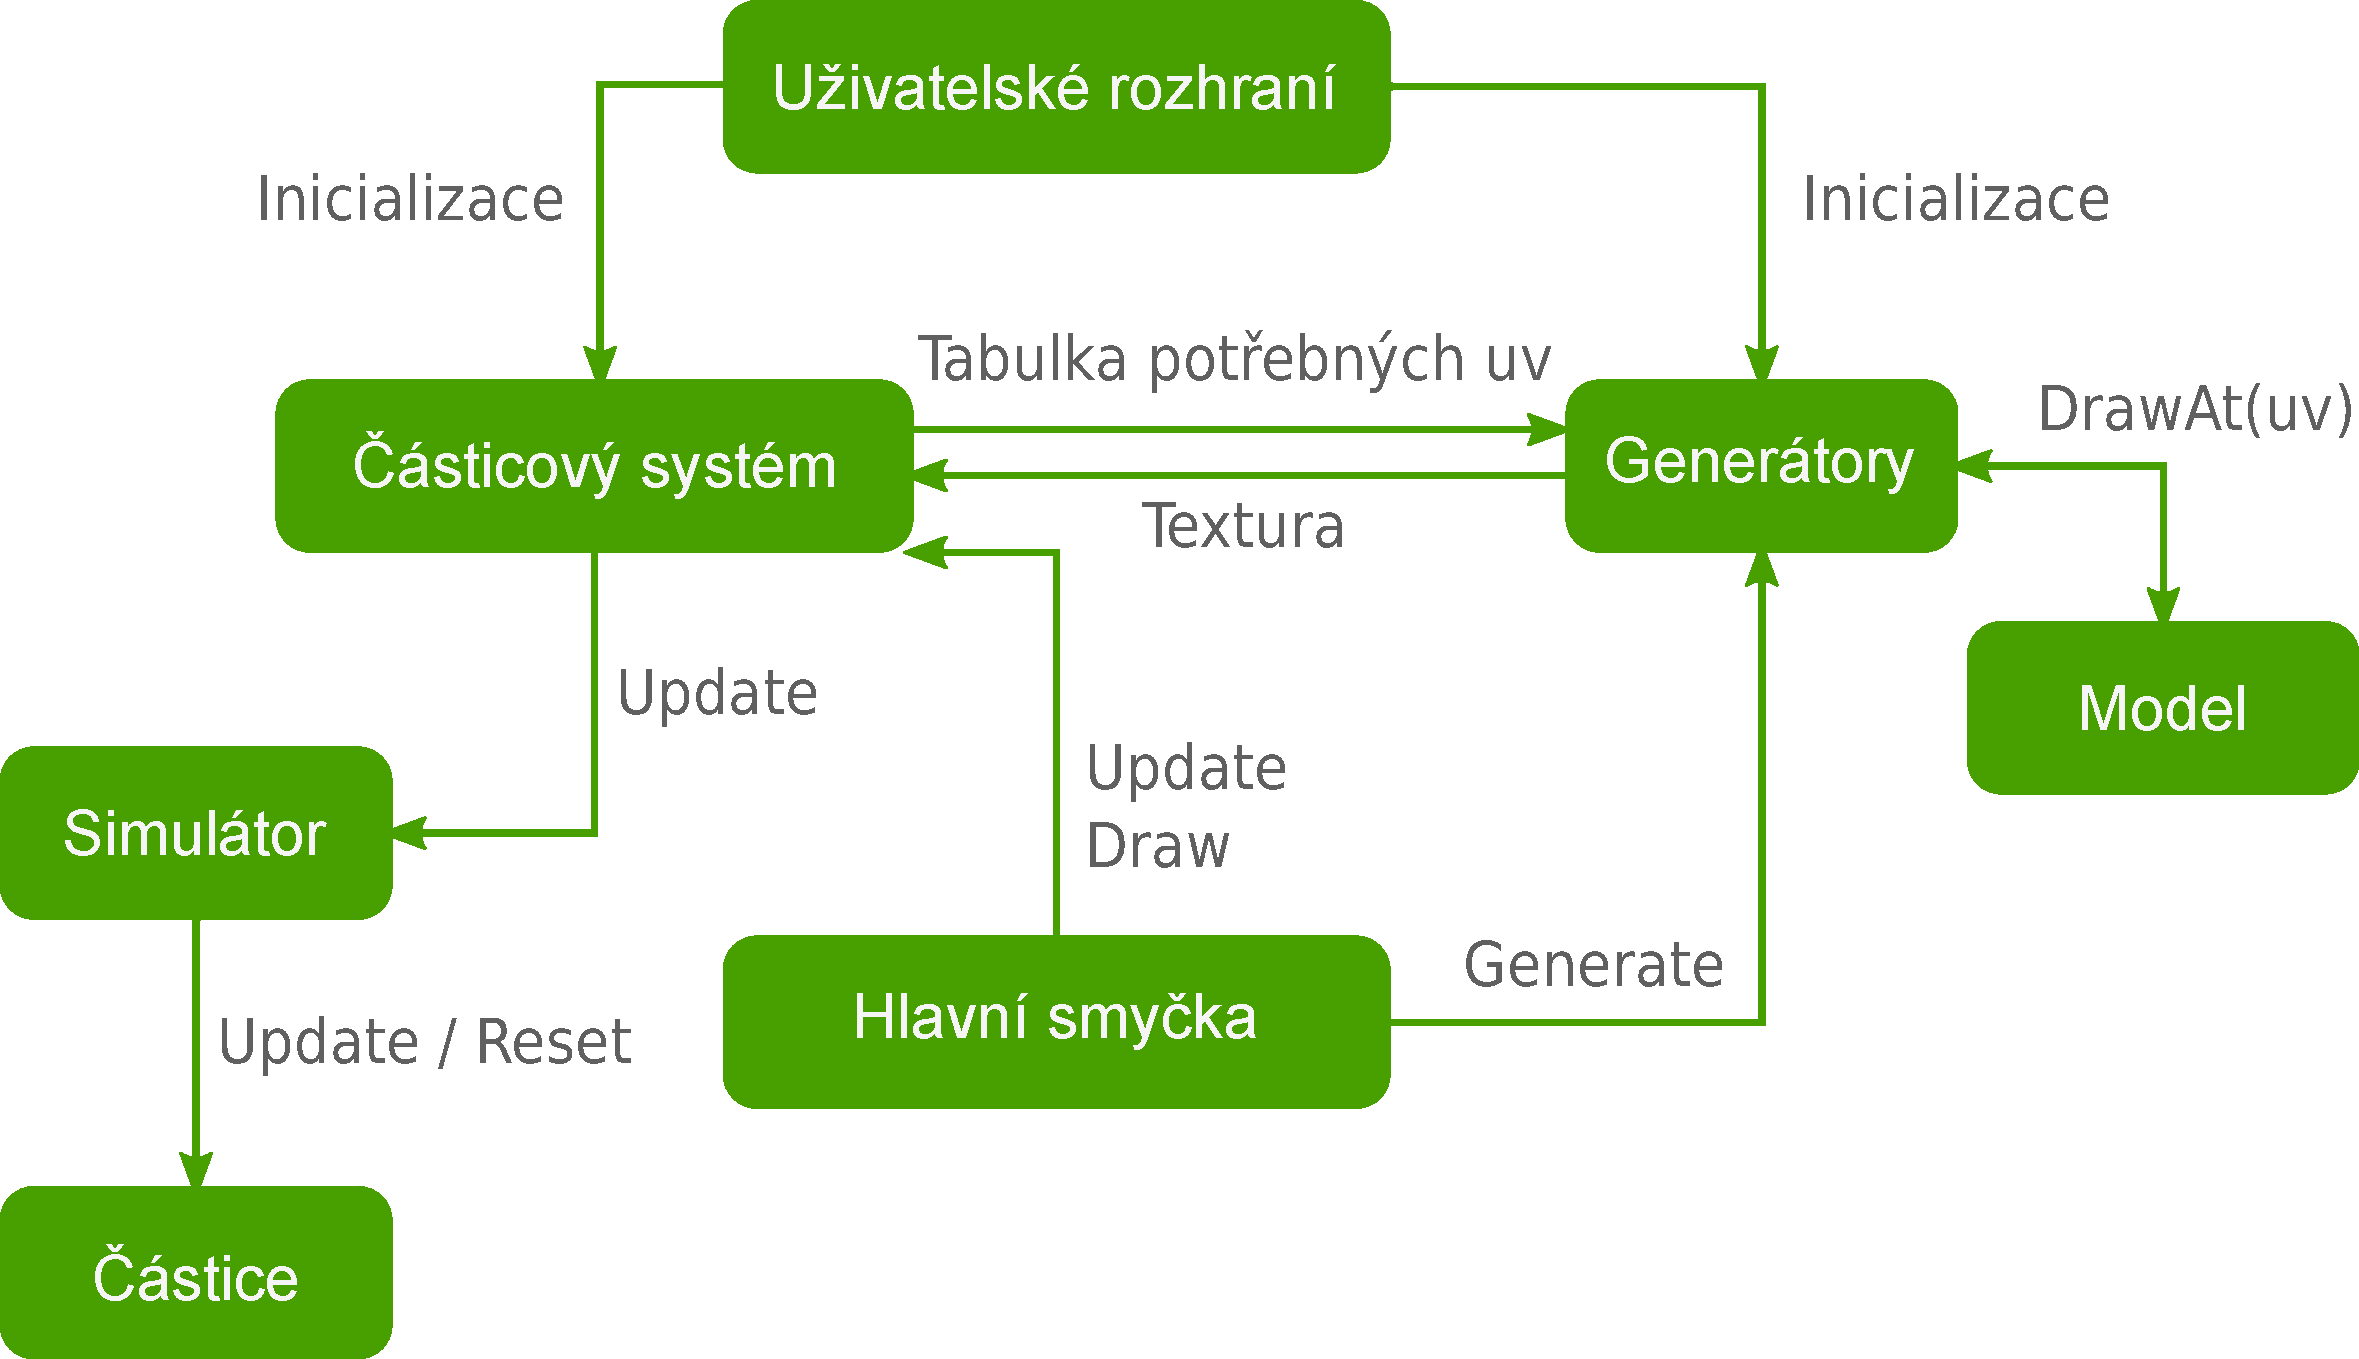
\includegraphics[width=1.0\textwidth]{obrazky-figures/diagrambpfull.pdf}
	\caption{Jednotlivé moduly nástroje a vztahy mezi nimi.}
	\label{fig:navrh_uml}
\end{figure}



\section{Architektura}
\label{sec_architecture}
Architektura nástroje je navržena tak, aby byla snadno rozšiřitelná. Jednotlivé části jsou tedy rozděleny na moduly, které zajišťují určitou funkcionalitu. Řada z~těchto modulů je navhrnuta tak, aby mohly být snadno nahrazeny a šla tak snadno změnit funkcionalita celého nástroje.
\subsection*{Grafické rozhraní} Slouží k~editování parametrů a přepínání možných scén. Může měnit vlastnosti simulace, jako jsou například síla gravitace, rychlost částice. Scény obsahují různorodé vizuální prostředí (například rozdílné skyboxy) a odlišné \texttt{částicové systémy} demonstrující různou funkcionalitu. Dále je možné měnit parametry generátorů, jako je například \emph{hustota} pořízení light field dat, nebo rozlišení výsledné textury. Grafické rozhraní také zajišťuje ovládání kamery.  
\subsection*{Částice} Každá částice obsahuje informace o~pozici a času života. Obsahuje také rozhraní \texttt{Reset} a \texttt{Update}. \texttt{Reset} uvede částici do počátečního stavu -- například při vypršení doby života. Obvykle jsou některé vlastnosti určeny stochasticky, aby docházelo k~chaotickému chování. \texttt{Update} ovlivňuje chování částice v~průběhu simulace. Obvykle mění pozici částice pro efekt pohybu. 

Při vytváření částicového systému je nutné specifikovat prototyp částice (podle návrhového vzoru \emph{Prototype}), který je poté použit při vytváření částic. Rozšířená částice tedy také obsahuje rozhraní \texttt{Clone} vytvářející kopii této částice. 

Jednotlivé částice jsou vykreslovány jako kamerou orientované billboardy. Textura těchto billboardů je tvořena rekonstrukcí dat zachyceného light fieldu. Výsledný objekt je velmi podobný billboardu typu impostor, avšak nemusí být při každé změně úhlu pohledu opět provedeno renderování (pokud se úhel pohledu již nachází v~mřížce). Navíc přechody mezi úhly jsou díky interpolaci plynulé.

\subsection*{Simulátor} Spravuje jednotlivé částice a zajišťuje jejich simulaci. Částice jsou vytvářeny z~daného prototypu pomocí rozhraní \texttt{Clone} a simulovány pomocí rozhraní \texttt{Update}. Při změně prototypu se všechny částice znovu inicializují. Modul také uchovává a aktualizuje simulační čas, který je při simulaci předáván částicím. Konkrétní chování vždy implementují samotné částice. 


\subsection*{Částicový systém} Tento modul spravuje celý částicový systém a vykresluje částice. Obsahuje rozhraní \texttt{Draw}, které částice vykreslí. Uchovává informaci o~dostupných texturách, vytvořených generátory a předává ji částicím. Která textura bude použita závisí na implementaci částice. 

Dalším úkolem částicového systému je vytvořit \texttt{Tabulku potřebných úhlů pohledu}. V~této tabulce jsou obsaženy všechny ${(u,v)}$ souřadnice, které částice potřebují ke korektnímu vykreslení. Jedná se o~souřadnice průniku úsečky procházející pozicí částice a pozicí kamery rovinou ${uv}$. Tato tabulka je po vytvoření předána generátorům. Proces vytváření a předávání tabulky je znázorněn na obrázku \ref{fig:uv-tabulka}.

\begin{figure}[H]
	\centering
		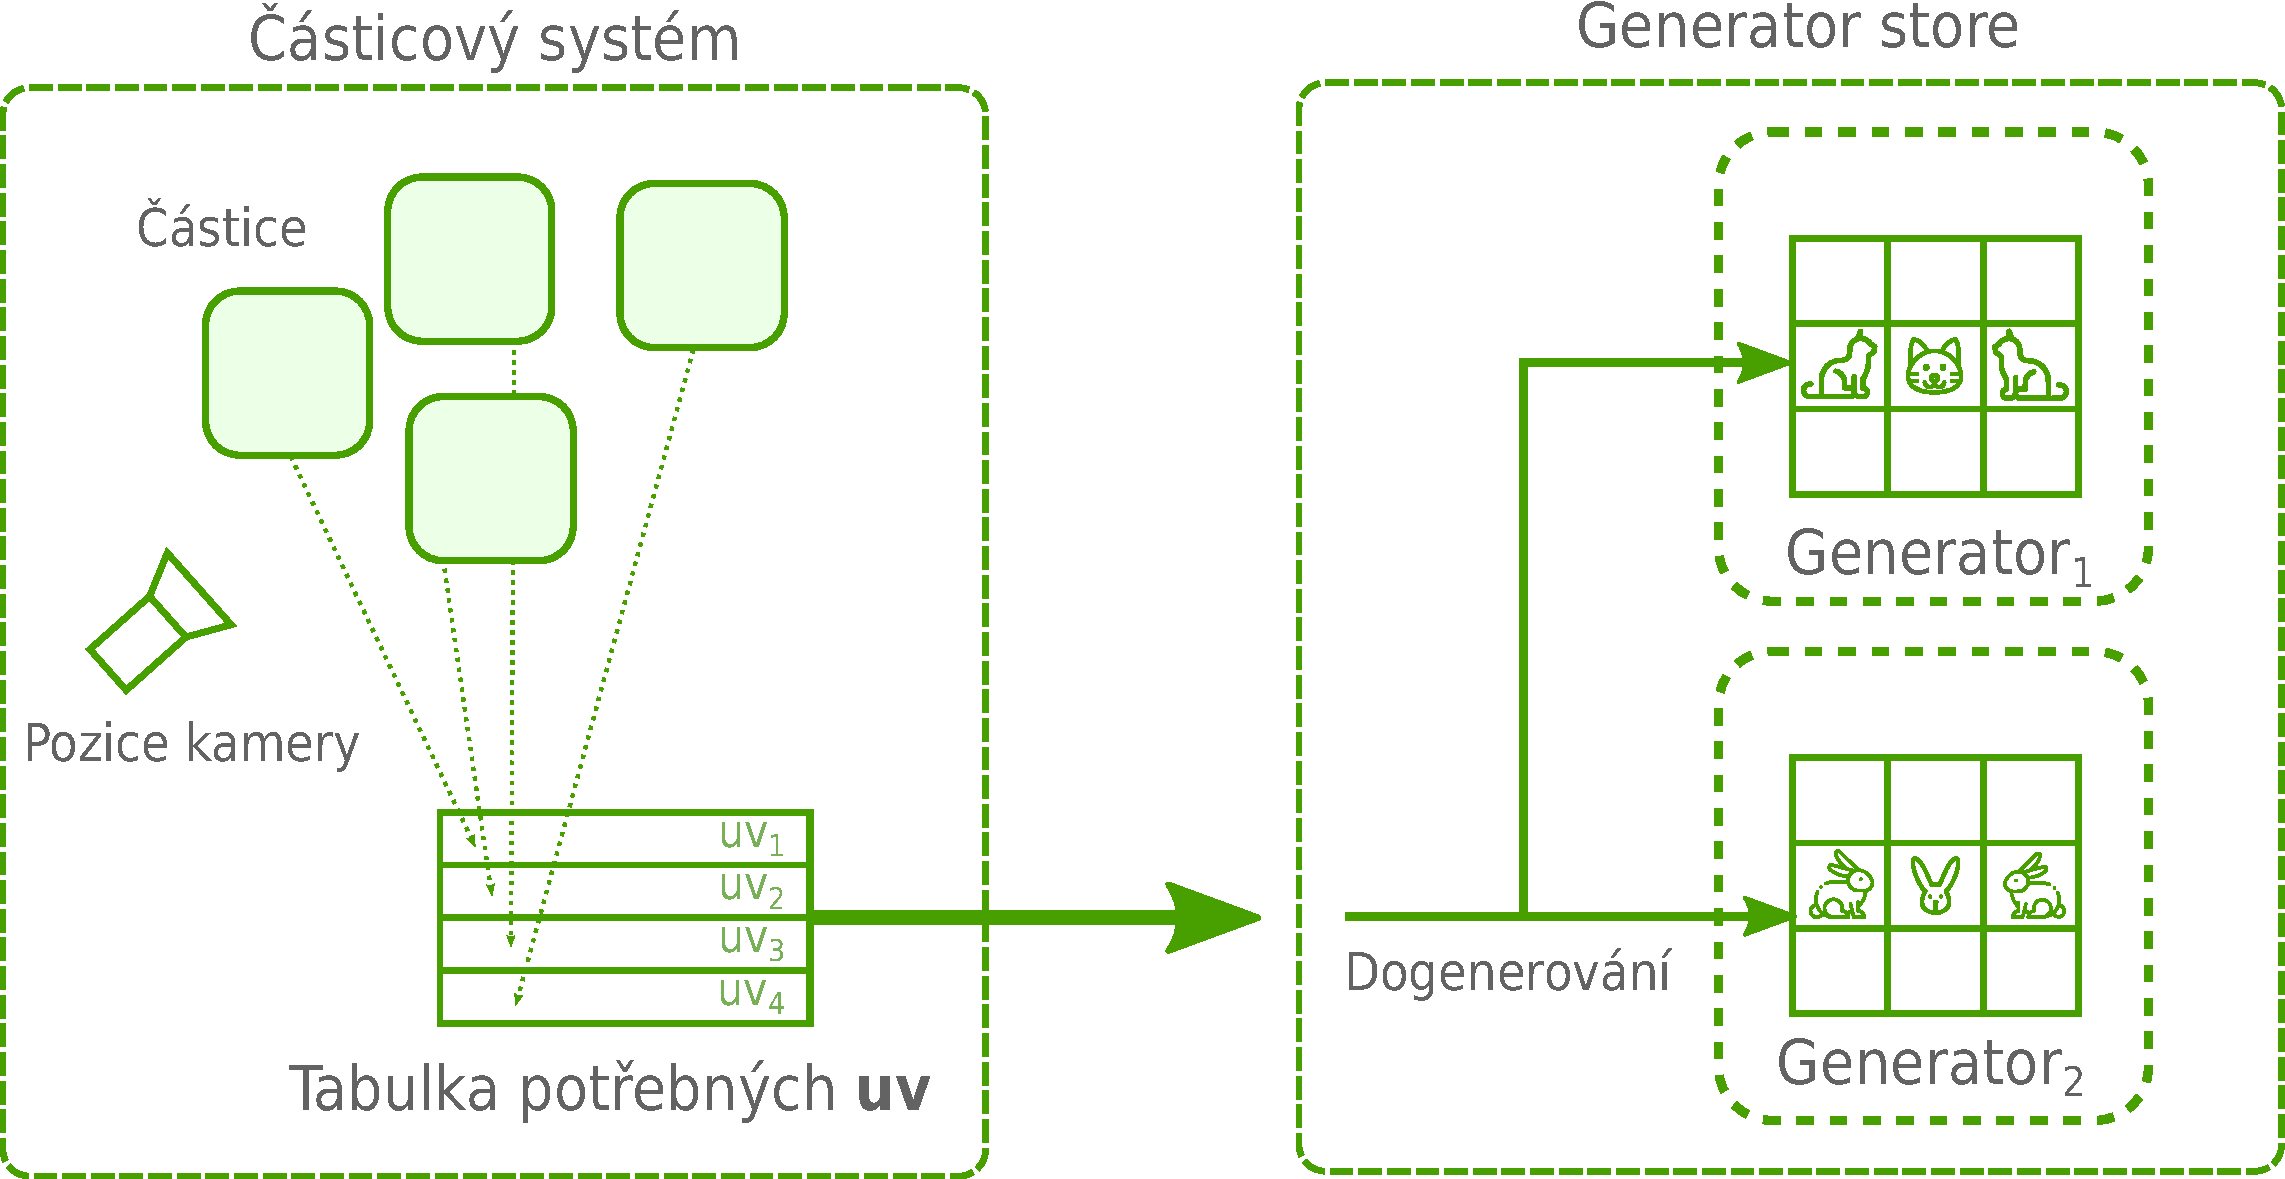
\includegraphics[width=1.0\textwidth]{obrazky-figures/uvdiagram.pdf}
	\caption{Vytváření tabulky s~potřebnými ${(u,v)}$ souřadnicemi obsahující jeden záznam pro každou částici a následné předání generátorům. Průběh doplnění cache tabulky a dogenerování dat light fieldu jsou více popsán v~sekci \ref{navrh-generator}.}
	\label{fig:uv-tabulka}
\end{figure}
\pagebreak
Tento modul také obsahuje rozhraní pro změnu parametrů částic a jejich simulací. To je například síla gravitace, rychlost částice, možnost její rotace nebo počáteční doba života. Dále je možné měnit parametry vykreslování, například použitý shader.

Konkrétní částice nejsou přímo součástí částicového systému, ale jsou uloženy a spravovány modulem \texttt{Simulátor}.

\subsection*{Generator Store} Jednoduchý modul zaštiťující práci s~generátory, vytvořený podle návrhového vzoru \emph{Store}. Poskytuje rozhraní pro práci se všemi používanými generátory. Umožňuje získat vytvořené textury a předává generátorům \texttt{Tabulku potřebných úhlů pohledu} vytvořenou částicovým systémem. Umožňuje měnit parametry jako jsou \emph{hustota} nebo rozlišení textury a \emph{speciální parametry}. Modul generátory nevytváří, pouze uchovává a spravuje. 

\subsection*{Generátor} 
\label{navrh-generator}
Vytváří data light fieldu. Při vytváření je nutné definovat \emph{model}, s~kterým má generátor pracovat. Generátor obsahuje rozhraní \texttt{Generate}, které vykresluje definovaný model pod různými úhly, a zachycuje tak data light fieldu, které ukládá do textury.

Data jsou uložena jako 2D pole obrázků reprezentující \((u,v)\) souřadnice, kde jednotlivé pixely reprezentují souřadnice ${(s,t)}$, jak je znázorněno na vizualizaci na obrázku \ref{fig:lightfield_reprezentation}. Tato data jsou uložena do textury. Rozměr tohoto pole je dále nazýván jako \textbf{hustota} a určuje míru vzorkování. Pokud je tedy například hodnota hustoty pět, bude mít výsledné pole pět obrázků na šířku i na výšku. Rovina ${(u,v)}$ sféricky obklopuje objekt, musí tedy být vzorkování dostatečné aby byly přechody mezi úhly plynulé. Příliš vysoké vzorkování může mít však velmi negativní efekt na objem potřebné paměti, a je tak nutné snížit kvalitu jednotlivých obrázků, což má dopad na výslednou kvalitu. 

Light field může být vygenerován celý, ještě před spuštením hlavní smyčky, nebo může být dokreslován postupně dynamicky za běhu. K~tomuto účelu slouží \texttt{Cache tabulka}. Tato tabulka obsahuje jeden záznam pro každou možnou ${(u,v)}$ souřadnici, její rozměry tedy odpovídají \emph{hustotě}. Každý záznam se může nacházet ve třech stavech: 
\begin{itemize}
    \item \texttt{Empty} - data nebyla vytvořena a není třeba je vytvářet,
    \item \texttt{Activated} - data nebyla vytvořena, ale je třeba je vytvořit,
    \item \texttt{Cached} - data již byla vytvořena.
\end{itemize}
Ve výchozím stavu jsou všechny záznamy ve stavu \texttt{Empty}. Pokud je záznam v~tomto stavu a částicový systém zaznamená v~\texttt{Tabulce potřebných úhlů pohledu} potřebu dokreslit dané ${(u,v)}$ souřadnice, tak je záznam přepnut do stavu \texttt{Activated}. V~tomto případě jsou při dalším generování data pro potřebné ${(u,v)}$ souřadnice doplněna do výsledné textury a záznam přepnut do stavu \texttt{Cached}. Poté již v~tomto stavu záznam setrvá. Ke generování tedy dochází pouze pro záznamy ve stavu \texttt{Activated}. Celý tento proces je znázorněn diagramem na obrázku \ref{fig:lftabulka}. Při změně \emph{speciálních parametrů} dojde k~vyresetování tabulky do výchozího stavu, a data se tak začnou přegenerovávat s~novými parametry. Může tak docházet k~dynamickým změnám za běhu. 

\begin{figure}[H]
	\centering
		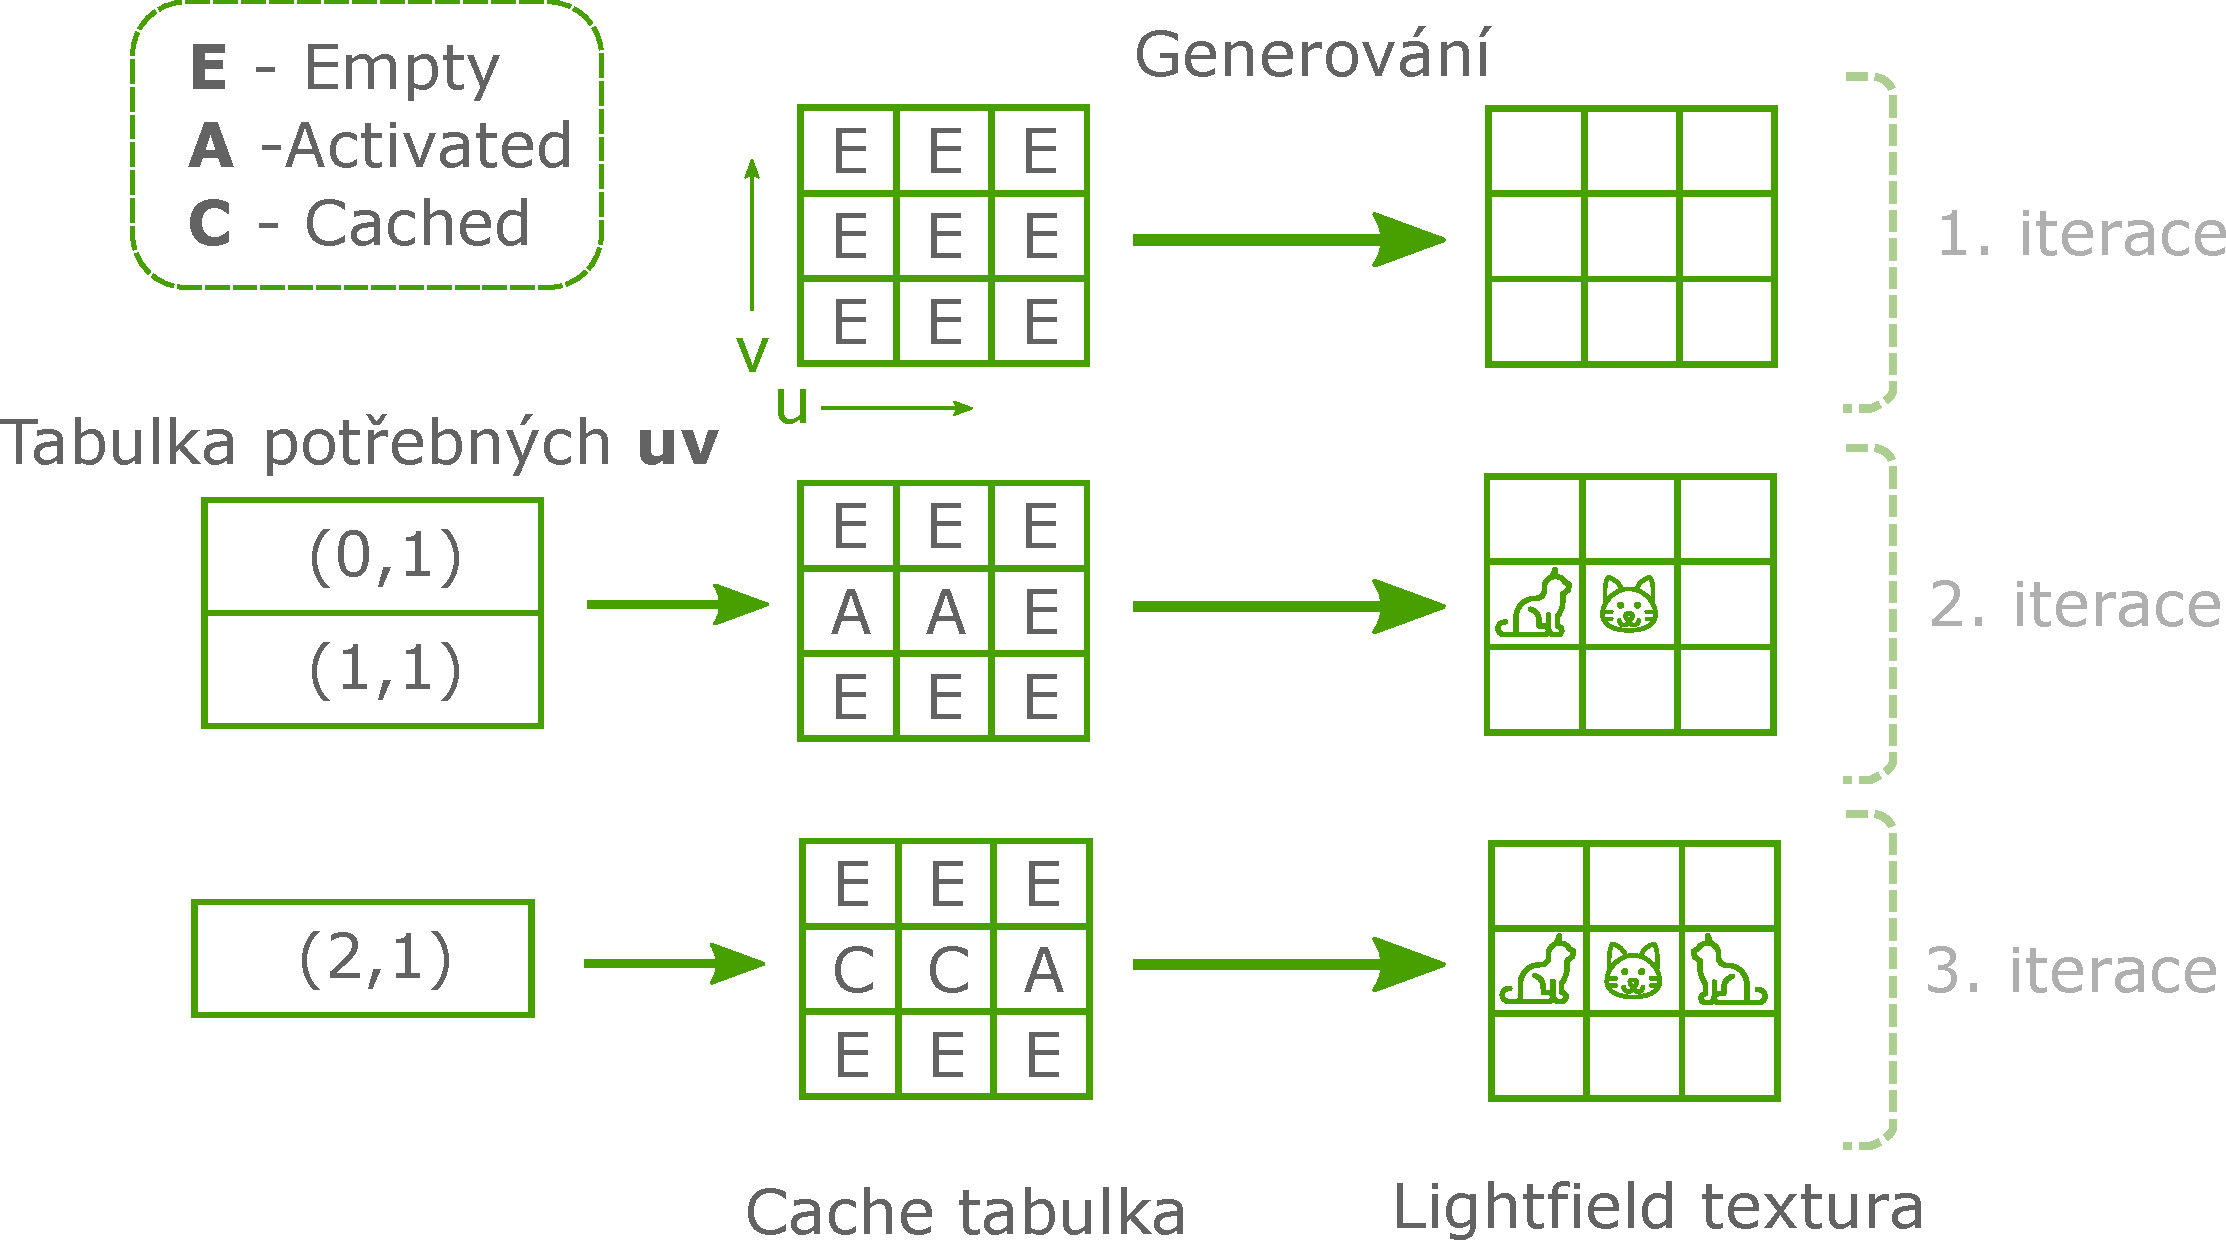
\includegraphics[width=1.0\textwidth]{obrazky-figures/lfdiagram_fixed.pdf}
	\caption{Diagram zobrazující navrhovaný dynamický způsob generování light field textury. Vstupem generátoru je tabulka potřebných ${(u,v)}$ souřadnic. Z~poskytnutých souřadnic je aktualizována cache tabulka. Ta generátoru signalizuje, na kterých souřadnicích je nutné texturu doplnit. V~diagramu jsou znázorněny tři iterace hlavní smyčky.}
	\label{fig:lftabulka}
\end{figure}


\subsection*{Model} Model obsahuje 3D objekt, ze kterého má být vytvářen light field. Musí obsahovat rozhraní \texttt{Draw}, které objekt vykreslí. Při vykreslování je nutné specifikovat rotační vektor, kterým má být objekt při vykreslování rotován. Tento vektor je využíván především modulem \texttt{Generator} při vytváření light filedu, kde je zapotřebí vykreslit objekt při různé rotaci. 

Dále je možné specifikovat parametry, které budou dále nazývány jako \textbf{speciální parametry}. To mohou být například parametry světla, které májí být při vykreslování modelu použito. Takové světlo lze po vytvoření light fieldu měnit pouze přegenerováním a bude dále nazýváno jako \textbf{statické světlo}. Dalším parametrym může být například statický rotační vektor, který bude vždy použit při vykreslování. 

Speciální parametry i způsob vykreslování rozhraním \texttt{Draw} jsou zavislé na konkrétní implementaci modulu a mohou se libovolně měnit v~podobě rozšíření. Měla by však vždy být dodržena funkcionalita rotování objektu podle rotačního vektoru, aby bylo možné light field vytvořit. 

\subsection{Rozšíření modulů}
Většinu modulů lze jednoduše rozšířit o~další funkcionalitu. Především se jedná o~chování částic a dynamickou změnu dat. Tato sekce popisuje, jakými způsoby lze navrhnuté modely rozšiřovat 

\textbf{Částici} lze rozšířit různými typy chování nahrazením metod \texttt{Update} a \texttt{Reset}. \texttt{Update} ovlivňuje způsob, jakým je částice simulována. Lze tak změnit časový průběh života částice. Změna rozhraní \texttt{Reset} může velmi snadno ovlivnit, jak jsou částice inicializovány. Změnou této metody lze například měnit generační tvar systému nebo nastavit počáteční směr a rychlost.

\textbf{Model} je možné rozšířit dvěma hlavními cestami. První rozšíření se týká objektu, který má model zobrazovat, což může například obnášet použitý shader. Dalším možným rozšířením jsou \textbf{speciální parametry} a jejich projev při vykreslování. Speciální parametr může být v~podstatě cokoliv, co ovlivní vykreslovaný model. Například by speciální parametr mohl být čas a model se po překročení jisté hodnoty změní. Projevem změny parametrů mohou tedy  být například různé transformace, deformace, změny textury, nebo i dokonce animace. Je však nutné brát v~potaz, že každá změna parametru vede k~překreslení light fieldu a časté překreslování může mít negativní dopad na výkon systému. 

Moduly generátor a částicový systém nejsou přímo určeny k~rozšíření. Je vhodnější je přímo nahradit vlastní implementací. Například generátor by bylo možné nahradit pouhou předvytvořenou texturou v~případě, kdy není třeba light field tvořit za běhu. Změna částicového systému může sloužit ke kompletní změně způsobu vykreslování, což může být užitečné například při srovnávání jiných metod vykreslování částicových efektů.

\section{Uživatelské rozhraní}
Grafické rozhraní slouží pro změnu různých parametrů částicového systému a generátorů. Dále také umožňuje měnit scény a jejich parametry. Návrh rozložení je znázorněn na obrázku \ref{fig:mockup_gui}. Kamera je součástí grafického rozhraní a je možné ji ovládat.

\begin{figure}[H]
	\centering
		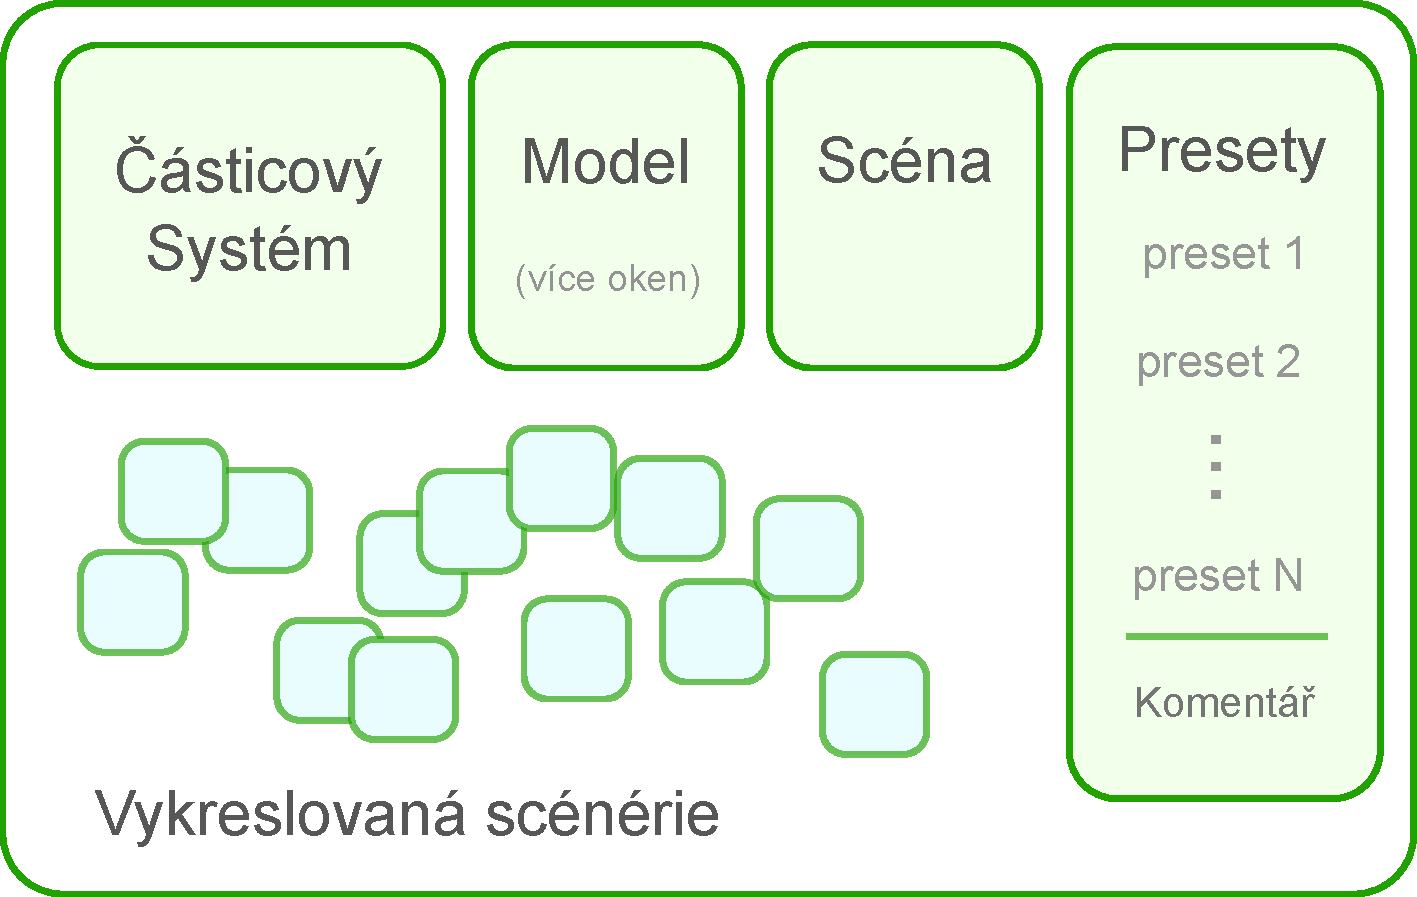
\includegraphics[width=1.0\textwidth]{obrazky-figures/uimockup.pdf}
	\caption{Diagram návrhu uživatelského rozhraní. V~nástroji se nacházejí čtyři hlavní okna sloužící k~úpravě parametrů a výběru scény. Všechna okna jsou částečně průhledná, přesunutelná a lze je pomocí klávesové zkratky vypnout a zapnout. Na pozadí je vykreslována samotná scéna.}
	\label{fig:mockup_gui}
\end{figure}

Grafické rozhraní je rozděleno na několik oken, které zajišťují různou funkcionalitu: 
\begin{itemize}
    \item \texttt{Částicový systém} -- umožňuje měnit různé parametry týkající se celého částicového systému. Kontrolky v~kategorii \emph{Simulace} umožňují měnit konkrétní vlastnosti simulace částic, jako je například rychlost, rotace atd. Kontrolky v~kategorii \emph{Vizuální} umožňují upravovat parametry generátorů. Jedná se především o~hustotu a rozlišení. Je zde také možnost zapnout zobrazování rámečku okolo částic pro snadné pozorování simulace, nebo zobrazit přímo celou light field texturu.
    \item \texttt{Model} -- těchto oken se může vyskytovat větší množství - jedno pro každý model. Obsahuje \emph{Speciální parametry} každého modelu. Jejich změna zapříčiní přegenerování light fieldu. Kontrolky v~kategorii \emph{Rotace} umožňují měnit statický rotační vektor modelu. Kategorie \emph{Světlo} obsahuje kontrolky umožňující vypnout či zapnout statické světlo a nastavit jeho parametry.
    \item \texttt{Scéna} -- umožňuje přepínat různé vlastnosti specifické pro aktuální scénu. Například vypínat či zapínat skybox nebo měnit jeho texturu. V~některých scénách je zde možné měnit vlastnosti světla.
    \item \texttt{Presety} -- slouží k~přepínání předvytvořených scén. Obsahuje také textový komentář k~aktuální scéně.
\end{itemize}

Kromě grafického rozhraní je také možné nástroj spouštět s~různými argumenty a přepínači z~příkazové řádky (dále CLI). Toto rozhraní umožňuje především upravit parametry simulace, lze zde například změnit počet částic nebo upravit rozlišení textury light fieldu. CLI je také možné využít pro změnu scény, avšak jen některé scény jsou takto přístupné. Je zaměřeno především pro účely měření pomocí měřícího nástroje, který aplikaci spouští s~různými argumenty a sleduje měřené metriky. Více informací o~tomto nástroji lze nalézt v~kapitole \ref{sec_benchmark_impl}.    

\section{Metodika měření}
\label{sec:methodology}
Pro ohodnocení navrhované metody vykreslování částicových efektů je nutné ji otestovat a změřit. Metoda by měla umožnit efektivně zobrazovat velké množství 3D objektů bez nutnosti je přímo renderovat. Každé měření musí být tedy vykonáno pro navrhovanou metodu i pro standardní způsob renderování 3D objektů, aby bylo možné srovnat, zda navrhovaná metoda opravdu přináší přínos. Součástí řešení je i dynamická změna vzhledu částic v~průběhu simulace, a tak je i tuto vlastnost nutné řádně změřit.

Kromě srovnávání je také žádoucí sledovat vliv různých parametrů na sledované metriky, například: různá složitost zobrazovaného objektu, počet částic a kvalita textury částic.
\subsection*{Sledované metriky}
Při měření je nutné korektně oba způsoby renderování srovnat. K~tomu lze využít několik metrik. Z~hlediska výkonu lze sledovat vytížení CPU a grafické karty, a především maximální dosažitelný počet vykreslovaných snímků za sekundu. Další důležitou metrikou je požadovaný objem systémové paměti a paměti grafické karty. 

Dále je nutné sledovat, zda navrhovaná metoda generuje vhodné vizuální výsledky. Vizuálně je tedy možné metody porovnat s~pomocí implementovaného nástroje. Alternativně lze také změřit podobnost vykreslených scén pomocí metod, jako jsou MSE, PSNR či SSIM\footnote{MSE - mean squared error, PSNR - peak signal-to-noise ratio, SSIM - structural similarity index measure }.
\subsection*{Způsob měření}
Jedním ze způsobů, jak dosáhnout co nejpodobnějšího výsledku pro srovnávání, je nahradit metodu \texttt{Draw} u~částicového systému tak, aby místo billboardů s~texturami přímo volala metodu \texttt{Draw} modelu, ze kterého je pořizován light field. Takto modul vykreslí objekt obsažený v~modelu pro každou částici. A~jelikož je simulace částic prováděna v~simulátoru, měl by tento částicový systém vypadat velmi podobně jako systém využívající light field. 

Vzhledem ke skutečnosti, že značná část sledovaných metrik je ovlivňována hardwarovými prvky, je nutné měření provést na větším počtu zařízení. Zejména je žádoucí pozorovat měření na nevýkonných zařízeních, aby se mohla projevit případná limitace objemu grafické paměti. Avšak nutná jsou i měření na výkonnějších sestavách, aby bylo možné odhadnout, jaký vliv bude mít budoucí vývoj hardwaru na využitelnost navrhované metody. Vzhledem k~vysokému počtu fragmentů, kde musí být provedeny náročné operace, lze předpokládat, že počet shaderových výpočetních jednotek bude mít velmi relevantní vliv na efektivitu.

\chapter{Implementace}
Tato kapitola se věnuje použitým technologiím a konkrétní implementaci nástroje. Jsou zde podrobně popsány jednotlivé moduly, jejich implementace a implementovaná rozšíření. Dále je také popsána implementace nástroje určeného pro měření.

Nástroj je tvořen pomocí jazyka \texttt{C++17}. K~zobrazování a k~práci s~grafickou kartou bylo použito rozhraní \texttt{OpenGL}. Pro matematické funkce a struktury byla využita knihovna \texttt{GLM}. Grafické rozhraní bylo vytvořeno za pomocí knihovny \texttt{NanoGUI}. Pro načítání 3D modelů v~různých formátech se využila knihovna \texttt{assimp}. Technologie použité pro vývoj testovacího nástroje jsou podrobněji popsány v~kapitole \ref{sec_benchmark_impl}.

Jelikož je nástroj tvořen pomocí jazyka \texttt{C++}, který umožňuje objektově orientované programování, jsou všechny moduly navrhnuté v~sekci \ref{sec_architecture} implementovány jako třídy. Některé byly však rozděleny do více menších tříd, aby kód více odpovídal SOLID principům.

K~vykreslování částicového systémů je využito několik výpočtů, které jsou částečně realizovány na CPU a částečně na grafické kartě. Výpočet $uv$ souřadnic pro texturu probíhá na CPU. Tyto souřadnice jsou využívány při interpolaci, jejíž výpočet probíhá na grafické kartě a je částečně rozdělen do vertexového a do fragmentového shaderu. Rotační matice pro billboarding je předpočítána na CPU a poté předána pomocí uniformní proměnné vertex shaderu, který provádí rotaci bodů. 

\section{Pořízení light fieldu}
Pořízení light fieldu zajišťují dle návrhu moduly \textbf{generátor} a \textbf{model}, které jsou implementovány jako vlastní třídy. Při vytváření generátoru je mu předán ukazatel na model, se kterým má pracovat. Je také specifikována počáteční \emph{hustota} a rozlišení textury light fieldu. Oba tyto parametry mohou být za běhu měněny pomocí funkcí \texttt{SetDensity} a \texttt{SetResolution}, které parametry změní a vyresetují \texttt{cache tabulku}, což zapříčiní překreslení textury light fieldu. 
\subsection{Model}
\label{sec:model_impl}
Model je třída zajišťující vykreslování 3D objektu a předává se pomocí chytrého ukazatele generátoru, který s~ní poté pracuje. Lze ji pomocí dědičnosti jednoduše rozšířit o~další funkcionalitu. 

Při inicializaci modelu je nutné specifikovat cestu souboru obsahující model. Pomocí knihovny \texttt{assimp} se načtou jednotlivé stěny (faces), vrcholy, normály a souřadnice textur. Tyto hodnoty jsou uloženy do příslušných bufferů. 

Model implementuje metodu \texttt{Draw}, která je označena jako virtuální, jelikož je určena k~přepsání při rozšiřování pomocí dědičnosti. Výstupem této metody je vykreslení objektu do aktivního framebufferu. Vstupem této metody je rotační vektor $r$ obsahující požadovanou rotaci po osách $x$ a $y$ v~radiánech. Tento vektor je využit generátorem při generování pod různými úhly při tvorbě light fieldu. Dalším vstupem je ukazatel na strukturu se \emph{Speciálními parametry}, které obsahují další informace:
\begin{itemize}
    \item Zda má být aplikováno tzv. \uv{statické světlo}. Jedná se o~světlo, kterým bude objekt osvícen již při vytváření light fieldu.
    \item Barva statického světla, pokud je zapnuto.
    \item Pozice statického světla, pokud je zapnuto.
    \item Statický rotační vektor, obsahující stupeň rotace po osách $x$, $y$ a $z$. Tento vektor není určen, narozdíl od vstupního vektoru funkce, pro rotaci při generování light fieldu, ale pro změnu orientace objektu k~dosažení požadovaného vzhledu.
\end{itemize}
Je předpokládáno, že změna těchto parametrů zapříčiní překreslení textury light fieldu, což je mimo jiné důvodem, proč je statický a vstupní rotační vektor oddělen. Tato struktura může být také rozšířena o~další parametry pomocí dědičnosti, ale současně musí být rozšířen i model o~požadovanou funkcionalitu.

Pro vykreslení jsou použity běžné shadery. Vertex shader pouze transformuje pozici vrcholů pomocí modelové, pohledové a projekční matice a interpoluje souřadnice textur a normál. Hodnoty světla jsou předány pomocí uniformních proměnných. Fragmentový shader aplikuje jednoduché osvícení (pokud je zapnuto) a nastaví texturu. Při vykreslení je připojen potřebný buffer a objekt je vykreslen pomocí funkce \texttt{glDrawElements}.
\label{sec:implemented_extensions}
V~nástroji je implementováno pouze jedno rozšíření modelu, které při vykreslování využívá jiného fragmentového shaderu. Tento shader nijak nevyužívá světlo a při vykreslování nenastavuje barvu fragmentů na barvu textury ale na hodnotu normál. Je využit ve scéně s~reálným světlem, která je popsána v~sekci \ref{sec:real_light_scene}. 
% Příklad objektu vykresleného tímto modelem lze nalézt na obrázku \ref{fig:normal_model}.

% \begin{figure}[H]
% 	\centering
% 	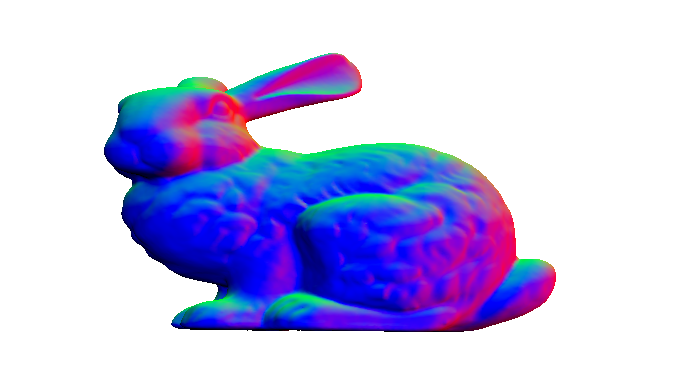
\includegraphics[width=0.45\textwidth]{obrazky-figures/normal_model.png}
% 	\caption{Rozšířený model, vykreslující normálové vektory s pomocí rgb kanálů. }
% 	\label{fig:normal_model}
% \end{figure}

\subsection{Generátor}
Generátor je modul zajišťující samotné vytváření light fieldu. Jeho funkcionalita je rozdělena do tří tříd:
\begin{itemize}
    \item \texttt{Generator} - hlavní třída obsahující ostatní a poskytující rozhraní pro práci s~light fieldem. 
    \item \texttt{CacheTable} - cache tabulka obsahující informace o~${uv}$ souřadnicích, jež je třeba do textury light fieldu doplnit.
    \item \texttt{GeneratorTexture} - třída obsahuje frame buffer, do kterého je vykreslen model. Následně je použit jako textura a přidán do light field textury.
\end{itemize}
Při inicializaci je nutné specifikovat \texttt{model} a \emph{Speciální parametry}, které je možné měnit kdykoliv za běhu. Na rozdíl od většiny tříd v~aplikaci nejsou tyto třídy určeny k~rozšíření a neobsahují tak virtuální metody. Rozšířit chování generátoru lze pomocí různých modelů.

Metoda \texttt{\textbf{Generate}} vykonává generování textury light fieldu. Textura je konceptuálně rozdělena na 2D pole, kde počet záznamů odpovídá předdefinované \emph{hustotě}. Přiklad plně generované textury lze nalézt na obrázku \ref{fig:lf_texture}. Pro každý záznam $uv$ je zavolána metoda \texttt{Draw} modelu s~určitým rotačním vektorem $r_{uv}$. Hodnota tohoto vektoru je určena vztahem \ref{eq:rvector}.


\begin{figure}[H]
	\centering
	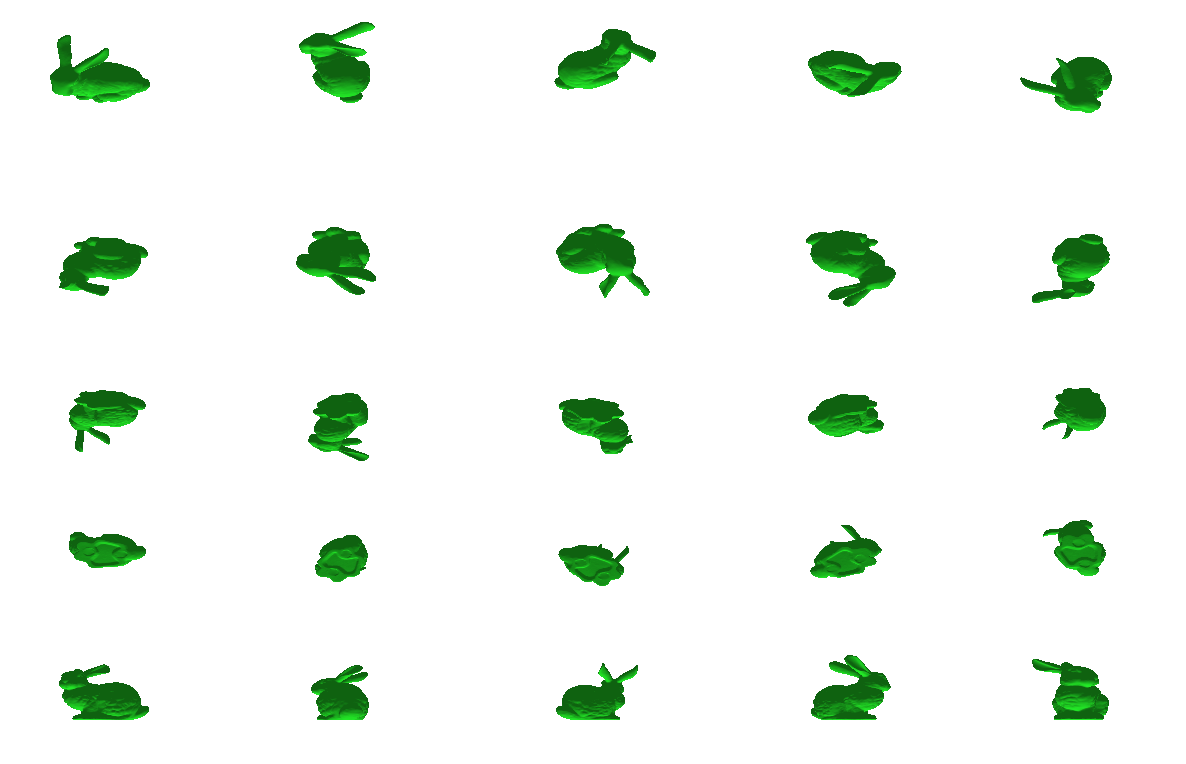
\includegraphics[width=0.85\textwidth]{obrazky-figures/lightfield_texture.png}
	\caption{Plně vygenerovaná textura light fieldu. Je vytvořena z~modelu, který obsahuje objekt \emph{Stanford bunny}. Textura má hustotu 5, což je velmi nízká hodnota. Obvyklá hustota textur v~implementovaných scénách se pohybuje v~rozhsahu 20 až 50.   }
	\label{fig:lf_texture}
\end{figure}
\begin{equation}
\label{eq:rvector}
{(r_x,r_y)_{uv} = \left(\frac{2\pi}{density} \times u, \frac{2\pi}{density} \times v\right)}
\end{equation}

Hodnoty $u$ a $v$ jsou indexy příslušného záznamu pole. Model je pomocí \texttt{GeneratorTexture} vyrenderován do textury a tato textura je nanesena na odpovídající $uv$ souřadnice v~textuře light fieldu. Pokud generování není přeskočeno, je patřičný záznam v~\texttt{Cache tabulce} označen jako \texttt{Cached}. Generování probíhá pouze pokud je záznam na daných souřadnicích označen jako \texttt{Active}. Tento proces je znázorněn Algoritmem \ref{alg:generator}.

\begin{algorithm}[H]
\caption{Generování dat light fieldu pomocí metody
\label{alg:generator}
\texttt{Generate} generátoru}
\begin{algorithmic}
\Procedure{Generate}{}
\For{\emph{u} $\gets \{0, 1, \dots (\emph{density}-1)\}$}
    \For{\emph{v} $\gets \{0, 1, \dots (\emph{density-1})\}$}
        \If{$CacheTable(u,v)$ is \texttt{Activated}} 
            \State $r \gets ComputeRotationVector(u,v)$ 
            \State $TextureResult \gets Model.Draw(r, \texttt{Special parameters})$
            \State $LightFieldData(u,v) \gets TextureResult$  \Comment{Add to light field texture}
            \State CacheTable(u,v) $\gets$ \texttt{Cached}
        \EndIf
    \EndFor
\EndFor
\State Return $LightFieldData$
\EndProcedure
\end{algorithmic}
\end{algorithm}

Třída také implementuje několik metod určených k~modifikaci \emph{Speciálních parametrů}. Každá tato metoda mimo jiné přepíše všechny záznamy v~\texttt{Cache tabulce} na výchozí hodnotu \texttt{Empty} a vymaže texturu light fieldu, což vede k~opětnému generování.


\subsubsection*{Textura light fieldu}
Textura light fieldu je vytvořena při inicializaci třídy a její velikost je dána určeným rozlišením. Nejdříve je vytvořen frame buffer a pomocí funkce \texttt{glFramebufferTexture} je mu přiřazena textura, do které bude ukládán výstup. Tento proces se opakuje při změně rozlišení textury. 

Při vykreslování se textura nepředává standardně pomocí \texttt{glBindTexture}, ale pomocí \textbf{Bindless textur}. Dokumentace \texttt{OpenGL}\footnote{https://www.khronos.org/opengl/wiki} uvádí, že se jedná o~rozšíření podporované většinou grafických karet podporujících verzi \texttt{OpenGL 4.0} a výše. Toto rozšíření umožňuje z~textury vytvořit \texttt{handle}, což je unikátní číslo reprezentující danou texturu. Poté lze \texttt{handle} například pomocí uniformních proměnných  předat fragmentovému shaderu, kde je možné s~pomocí této hodnoty vytvořit \texttt{sampler2D} a s~texturou přímo pracovat bez nutnosti bindování. Výhodou tohoto přístupu je možnost snadného současného využití předem neurčeného množštví textur.

Generátor při vytváření textury vygeneruje i \texttt{handle} a označí texturu jako \emph{residentní}, což k~ní umožní přístup z~fragmentového shaderu. Před vykreslováním částicového systému se pouze předají všechny generátory a je na implementaci fragmentového shaderu částice si zvolit, který \texttt{handle} použije. 

Pro texturu light fieldu je také použito \textbf{mipmapování}. Jeho hlavní výhodou je v~případě light fieldu redukce aliasingu a urychlení vykreslování. Konkrétní urychlení bylo součástí uskutečněných měření. Nevýhodou použití mipmapování je nutnost generování mipmap při každé změně textury. Při volání metody \texttt{Generate} je mipmapa generována pouze pokud proběhlo alespoň jedno vykreslování modelu, takže při ustáleném stavu, když již není textura měněna, tento problém odpadá.

\section{Zobrazení částicového systému}
Vykreslování částicových efektů zajišťují moduly \textbf{Částicový systém} a \textbf{Částice}, které jsou implementovány jako třídy. Čásice především uchovává informace nezbytné pro její vykreslení a samotné vykreslování zajišťuje částicový systém. 

Částice jsou vzhledem k~jejich vysokému počtu vykreslovány pomocí \textbf{instancování}. Každá částice je kamerou orientovaný billboard, jedná se tedy o~pouhý čtverec, který je rotován směrem ke kameře.  

Při inicializaci se vytváří nezbytné buffery. Nejdříve jsou vytvořeny buffery, které jsou sdílené pro všechny instance. Jedná se o~buffer obsahující vrcholy obdélníku a souřadnice textury. Dále je vytvořeno několik bufferů, které mají odlišnou  hodnotu pro každou texturu:
\begin{itemize}
    \item Pozice částice -- obsahuje $(x,y,z)$ souřadnice instance částice v~prostoru. Do tohoto bufferu se při každém průběhu renderovací smyčky ukládají pozice všech částic. 
    \item \texttt{Handle} textury -- obsahuje \texttt{handle} textury, které má částice využívat. Hodnoty tohoto bufferu se mohou, ale nemusí, měnit za běhu. 
    \item $(u,v)$ souřadnice -- souřadnice průsečíku úsečky směřující od kamery k~aktuální instanci s~rovinou $uv$. Tyto souřadnice jsou vypočítány při tvorbě \texttt{tabulky potřebných uv}. Vypočtené souřadnice jsou poté předány \texttt{cache tabulce} a konkrétním částicím, a následně uloženy do tohoto bufferu.
\end{itemize}
Aby byly hodnoty bufferu korektně rozděleny mezi částice, je dle referenčních stránek \texttt{OpenGL}\cite{glrefpages} nutné vytvořit dělič, který rozdělí hodnoty mezi instance. Ten lze vytvořit pomocí funkce \texttt{glVertexAttribDivisor} pokud je buffer v~aktuálním kontextu. 

Při každém vykreslování je nutné specifikovat hodnoty jednotlivých uniformních proměnných pro použité shadery. Jedná se o~modelovou, pohledovou a perspektivní transformační matici. Pohledová matice je vytvořena instancí třídy \texttt{Camera}, kterou spravuje uživatelské rozhraní.

\subsection{Mapování textury}
\label{sec:texture_mapping}
V~sekci \ref{sec:lightfield_zobrazeni} je uvedeno, že při nanášení light fieldu lze využít pohledovou matici a mapování textur pro určení $(u, v, s, t)$ souřadnic. Jelikož je light field pořizován sféricky, pro určení $(u, v)$ souřadnic je proto možné využít standardní sférické mapování, například podle vztahu \ref{eq:uvmaping}, jenž je popsán v~knize \emph{Moderní počítačová grafika} \cite[kapitola 13.1.1]{zara2004moderni}. Souřadnice $(x,y,z)$ budou dále označovány jako bod $P$.
\begin{equation}
\label{eq:uvmaping}
    \begin{array}{lll}
        u& =& \left\{ 
        \begin{array}{ccl}
        & \frac{1}{2\pi}arccos(\frac{x}{\sqrt{x^2 + z^2}}) & \text{pro } z~\leq 0 \\
        1 - & \frac{1}{2\pi}arccos(\frac{x}{\sqrt{x^2 + z^2}}) & \text{pro } z~> 0
        \end{array} 
        \right. 
        \\[1cm]
        v& =& 0.5 + \frac{1}{2\pi}arcsin(y)
    \end{array}
\end{equation}
 Bod $P$ je průsečík jednotkové sférické plochy $uv$ se středem $S$ a přímky směřující bodu $S$ k~pozici kamery $C$. Jeho souřadnice jsou tedy určeny vztahem \ref{eq:bodp}. Bod $S$ odpovídá pozici konkrétní částice v~prostoru. Tento výpočet probíhá ve fázi tvorby \texttt{tabulky potřebných uv} v~třídě částicového systému.
\begin{equation}
\label{eq:bodp}
      P_{xyz} = normalize(C_{xyz} - S_{xyz})
\end{equation}

Souřadnice ${(s, t)}$ jsou mapovány přímo na jednotlivé fragmenty výsledného billboardu. Míra vzorkování je omezena pořizovací \emph{hustotou}, a je tedy nutné mezi vzorky interpolovat, jak je popsáno v~sekci \ref{sec:lightfield_zobrazeni}. Byla použita metoda bilineární interpolace, jejíž vypočet opět vychází z~knihy \emph{Moderní počítačová grafika} \cite[kapitola 22.6.4]{zara2004moderni}. Tento vztah byl rozdělen na dvě části. První část, určená rovnicí \ref{eq:inter_first}, je vypočítána ve vertex shaderu a poté předána fragmentovému shaderu. Dojde tedy k~hardwarové interpolaci hodnot ${w_1}$, ${w_2}$ a ${w_3}$. Tento postup ušetří výpočetní kroky vzhledem k~faktu, že při vykreslování billboardu je počet vrcholů značně měnší než počet fragmentů. Druhý vypočet, určený rovnicí \ref{eq:inter_second}, je prováděn ve fragmentovém shaderu pro každý barevný kanál. Výsledné hodnoty jsou i výslednou barvou fragmentu.   

\begin{equation}
\label{eq:inter_first}
    w_1 =  \frac{|\mathbf{Q_{AB}} - \mathbf{A}|}{|\mathbf{B} - \mathbf{A}|}, \quad
    w_2 =  \frac{|\mathbf{Q_{CD}} - \mathbf{C}|}{|\mathbf{D} - \mathbf{C}|}, \quad
    w_3 =  \frac{|\mathbf{Q} - \mathbf{Q_{AB}}|}{|\mathbf{Q_{CD}} - \mathbf{Q_{AB}}|} 
\end{equation}
\begin{equation}
\label{eq:inter_second}
\begin{array}{llcll}
    h(\mathbf{Q_{AB}})& =& h(\mathbf{A}) + (h(\mathbf{B}) - h(\mathbf{A})) & \times &  w_1 \\[0,2cm]
    h(\mathbf{Q_{CD}})& =& h(\mathbf{C}) + (h(\mathbf{D}) - h(\mathbf{C})) & \times & w_2 \\[0,2cm]
    h(\mathbf{Q})& =& h(\mathbf{Q_{AB}}) + (\mathbf{h(Q_{CD}}) - h(\mathbf{Q_{AB}})) & \times &  w_3
\end{array}
\end{equation}
\pagebreak

Bod $Q_{AB}$ se nachází mezi bodem $A$ a $B$ a bod $Q_{CD}$ mezi body $C$ a $D$. Bod $Q$ se nachází mezi těmito dvěma body. Jejich pozice vychází ze souřadnic $(u,v)$ vypočítaných při mapování a jsou určeny rovnicemi \ref{eq:inter_points}.
\begin{equation}
\label{eq:inter_points}
\begin{array}{c}
    \mathbf{Q} =  (u,v) \times \text{hustota}, \quad
    \mathbf{Q_{AB}}  =  (Q_x, A_y), \quad
    \mathbf{Q_{CD}}  =  (Q_x, C_y) \\[0,5cm]
    \mathbf{A}  =  floor(Q), \quad
    \mathbf{B}  =  (C_x, A_y), \quad
    \mathbf{C}  =  (A_x + 1,A_y + 1), \quad
    \mathbf{D}  =  (A_x, C_y)
\end{array}
\end{equation}
A~jejich hodnoty $h()$ jsou hodnoty jednotlivých barevných kanálů. Pro bod $\mathbf{A}$ je hodnota určena rovnicí \ref{eq:inter_pointvals} a výpočet je stejný i pro body $\textbf{B}$, $\textbf{C}$ a $\textbf{D}$. \texttt{Tex} označuje pozici na billboardu a funkce \texttt{texture()} vrací barevné kanály \emph{rgba} z~určené textury. Textura je určena pomocí \texttt{handle}.
\begin{equation}
\label{eq:inter_pointvals}
\begin{array}{c}
    h(\mathbf{A})  =  texture\left(\texttt{handle}, \text{Tex}_{xy} + \frac{\mathbf{A}}{\text{density}}\right)

\end{array}
\end{equation}

Hlavní problém sférického mapování textury nastává v~momentě, kdy se souřadnice bodu $P$ příliš přiblíží k~pólům koule. Vznikne tak zkreslení, které je naznačeno na obrázcích \ref{fig:lf_baduv_mapping}. V~implementovaných scénách je koule vždy rotována tak, aby byly póly vždy co nejvíce vzdálené a ke zkreslení tak nedocházelo. 
\begin{figure}[H]
	\centering
	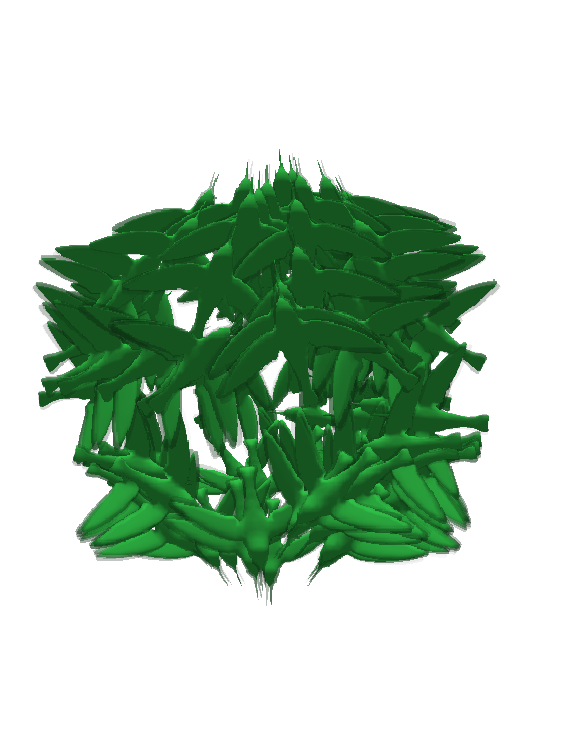
\includegraphics[width=0.45\textwidth]{obrazky-figures/uv_bad.png}
	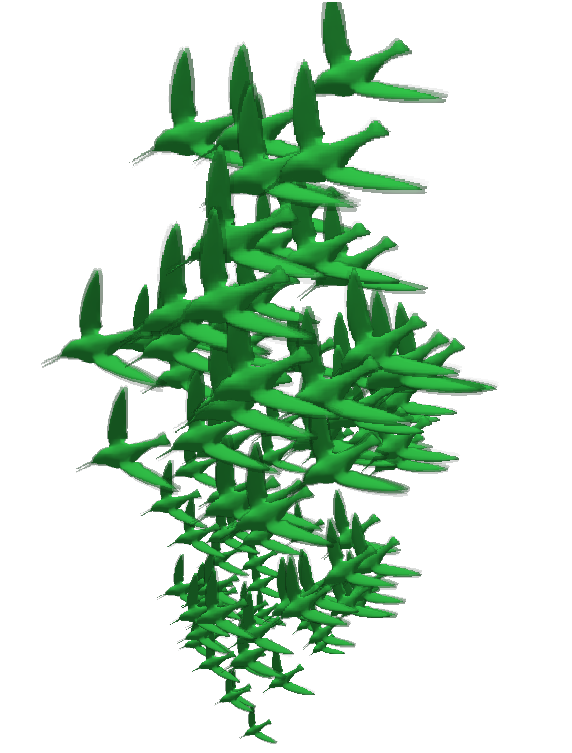
\includegraphics[width=0.45\textwidth]{obrazky-figures/uv_gut.png}
	\caption{Na levém obrázku je vyobrazen částicový systém, kde se kamera nachází velmi blízko pólů sférických ploch obklopujících částice, jenž slouží k~výpočtu $(u,v)$ souřadnic. Na pravém obrázku se nachází stejný částicový systém, ale kamera je od pólů dostatečně vzdálena.  }
	\label{fig:lf_baduv_mapping}
\end{figure}

\subsection{Částice}
Každá instance částice se skládá z~několika vrcholů, které dohromady tvoří čtverec. Vrcholy tohoto čtverce jsou ve vertex shaderu rotovány tak, aby vznikl kamerou orientovaný billboard. Tato rotace probíhá dle metody popsané v~sekci \ref{sec:camoriented_billboard}. Normálový vektor kamery $n$ je získán z~pohledové matice. 

Částice uchovává \texttt{handle} textury, který má být použit, a přidělené $(u,v)$ souřadnice. Také zajišťuje, aby byly udrženy v~rozsahu $(0,1)$. Pokud je rozsah překročen či podkročen, je hodnota rotována zpět do rozsahu. Například souřadnice s~hodnotou $1.3$ budou transformovány na $0.3$.
Pro částice jsou implementovány dva různé shadery, které lze v~částicovém systému přepínát. První je obyčejný, obsahuje vertex shader, který orotuje vrcholy a spočítá první část interpolace. Fragmentový shader načte poté zvolenou texturu pomocí \texttt{handle} a dokončí interpolaci. Pseudokód implementace shaderu je vyjádřen výpisem \ref{code:vertexp}.
\begin{lstlisting}[caption={Pseudokód vertex shaderu částic (zjednodušeno)}, label={code:vertexp}, language=C]
void main()
{
    // vertex position
    mat3 rotation = calculate_rotation(camera);
    vec3 position = rot * vertex_position;
    vec4 word_space = view * model * vec4(vertex_position, 1.0);
    word_space += view * model * vec4(particle_position, 1.0);
    vec4 screen_pos = projection * word_space;
    gl_Position = screen_pos;
    // begin interpolation
    vec2 uv = particle_uv;
    vec2 pos = Tex.xy;
    A, B, C, D = create_points(uv * density);
    Weights = calculate_interpolation((A,B,C,D));
    TexturePoints = pos + (A,B,C,D) / density;
}
\end{lstlisting}
Implementace fragmentového shaderu je naznačeta algoritmem \ref{code:fragp}. Dojde pouze k~dokončení interpolace
\begin{lstlisting}[caption={Pseudokód fragmentového shaderu částic (zjednodušeno)}, label={code:fragp}, language=C]]
uniform uint64_t texture_samples[MAX_TEXTURES];
void main() {
    sampler2D u_texture = sampler2D(texture_samples[TextureHandle]);
    A, B, C, D = TexturePoints;
    point_colors = texture(u_texture, (A, B, C, D));
    FragColor = bilinear(point_colors, Weights);
}
\end{lstlisting}
V~rámci rozšíření je implementován ještě další fragmentový shader, který využívá dvou textur. První je totožná jako v~běžném shaderu a druhá obsahuje objekt s~vyrenderovanými normálami, k~čemuž je použit rozšířený model popsaný v~sekci \ref{sec:model_impl}. Tyto normály jsou použity k~výpočtu světla pro každý fragment v~reálném čase. 
% \begin{lstlisting}[caption={Pseudokód rozšířeného fragmentového shaderu částic (zjednodušeno), aplikující světlo v reálném čase}, label={code:fragp_light}, language=C]]
% uniform uint64_t texture_samples[MAX_TEXTURES];
% void main() {
%     // base color
%     sampler2D u_texture = sampler2D(texture_samples[TextureHandle]);
%     A, B, C, D = TexturePoints;
%     point_colors = texture(u_texture, (A, B, C, D));
%     vec4 color = bilinear(point_colors, Weights);
    
%     // normal
%     // load second texture with normals
%     u_texture = sampler2D(texture_samples[TextureHandle + 1]);
%     A, B, C, D = TexturePoints;
%     point_colors = texture(u_texture, (A, B, C, D));
%     vec4 normal = bilinear(point_colors, Weights);
    
%     // light calculation
%     normal = normalize(normal)
%     light_direction = light_position - TexPosition;
%     vec3 diffuse = dot(normal, light_direction) * light_color;
%     FragColor = calculate_light(color,diffuse) // + ambient, speculat etc.
% }
% \end{lstlisting}
\subsection{Částicový systém}
\label{sec:impl_particles}
Tato třída zajišťuje inicializaci všech bufferů, načtení shaderů a samotné vykreslování. Poskytuje také rozhraní k~změně různých parametrů simulace. Další velmi významná úloha této třídy je tvorba a předání \texttt{tabulky potřebných uv}.

Tento výpočet je popsán v~sekci \ref{sec:texture_mapping}. Souřadnice $(u,v)$ jsou spočítány pro každou částici. Vstupem funkce pro tvorbu tabulky je třída \texttt{Generátor store}. Po dokončení tvorby tabulky je předána právě této třídě, která ji postupně předá každému vlastněnému generátoru. Generátory postupně tabulku procházejí a nastavují záznamy v~\texttt{Cache tabulce} na odpovídajících souřadnicích do stavu \texttt{Activated}. 

Při vykreslování částice probíhá interpolace mezi nejbližšími záznamy. Není proto možné do \texttt{Cache tabulky} vložit pouze záznamy obsažené v~\texttt{tabulce potřebných uv}, jelikož by mohlo dojít k~situaci, kdy částice při interpolaci částečně využívá i vedlejší záznam, který však ještě nebyl vygenerován, a tak v~textuře chybí. Musí být proto v~\texttt{Cache tabulce} aktivovány i všechny nebližší záznamy.

V~implementaci třídy není předpokládáno, že by byla rozšiřována, jelikož lze chování velmi jednoduše rozšířit pomocí různých prototypů částice. Vizuální stránku lze rozšířit pomocí modelu a použití jiného shaderu. V~nástroji je však implementována třída, která zcela nahraje částicový systém. Třída je nazvána \texttt{standard3DParticles} a nahrazuje vykreslování tak, že místo billboardových částic jsou jednotlivé částice skutečné 3D objekty. 

Primární účel této třídy je možnost srovnat a změřit vizuální a výkonnostní rozdíl mezi navrhovanou metodou využívající light field a metodou klasického 3D vykreslování. Při inicializaci je nutné specifikovat \texttt{model}, jehož objekt bude vykreslován, a parametry částic. Stejně jako u~light field částicového systému, je i zde použito instancování a je využit stejný simulátor.   
\section{Simulace}
Další důležitou součástí nástroje je simulace částic. Je téměř zcela oddělená od vykreslování a je ji tak možné využívat nezávisle, nebo například před spuštěním předsimulovat scénu, aby se již systém nacházel v~přirozeném stavu. 

Část simulační logiky je implementována ve třídě \texttt{Simulátor} a část implementuje přímo částice. Simulátor uchovává list všech vytvořených částic. Částice jsou vytvářeny z~prototypu částice. Ten může být specifikován pomocí metody \texttt{SetParticlePrototype}, která zničí všechny částice a vytvoří je z~poskytnutého prototypu. Poskytuje také metodu \texttt{Reset}, jejímž vstupem jsou \emph{parametry částice}. Metoda vyresetuje všechny částice a přiřadí jim poskytnuté parametry. 

\texttt{Parametry částice} je struktura obsahující různé parametry týkající se vlastností simulace. Například je zde síla a směr gravitace, rychlost a doba života částice nebo možnost zapnout jejich náhodnou počáteční rotaci. Tyto parametry je pomocí dědičnosti možné obohatit o~další. 

Metoda \texttt{Update} aktualizuje simulační čas a zavolá metodu \texttt{Update} každé částice. Vstupem této metody je právě simulační čas. U~výchozí částice proběhne kontrola, zda částice nedošla na konec své životnosti. Pokud ano, je zavolána metoda \texttt{Reset}, která ji restartuje. Pokud ne, je zavolána metoda \texttt{UpdatePhysics}, která pouze zavolá metodu  \texttt{SimulateMovement}. Tato metoda provede základní simulaci pohybu. Ten spočívá pouze v~pohybu ve směru částice, který je ovlivněn gravitací a případnou rotací. Všechny zmíněné metody částice jsou označeny jako virtuální a mohou být tedy jednoduše pomocí dědičnosti upraveny.

\section{Implementované scény}
V~nástroji je implementováno několik různých scén, mezi kterými lze volně přepínat. Jejich cílem je demonstrovat možnosti navrhované metody při různých rozšířeních. V~nástroji je obsaženo několik scén, jež jsou dostupné pouze přes CLI, jelikož jsou určeny pouze pro měření výkonu pomocí měřícího nástroje. V~nástroji je také možné nalézt stručný komentář popisující specifika každé scény.
\subsection*{Výchozí scéna}
Scéna demonstruje výchozí chování částicového systému. Obsahuje pouze jeden generátor, který používá výchozí model. Obsahuje malé množství částic, jelikož se jedná o~počáteční scénu. Pokud by byla počáteční scéna příliš komplikovaná, bylo by náročné s~nástrojem pracovat na velmi nevýkonných sestavách. 
\subsection*{Podzim}
Scéna na obrázku \ref{fig:ps_podzim} obsahuje podzimní scenérii, kde je s~pomocí částicového systému vytvořen efekt padajícího listí. K~tvorbě efektu byli použity tři generátory obsahující výchozí model. Každý generátor obsahuje list jiné barvy a rotace.  

\begin{figure}[H]
	\centering
	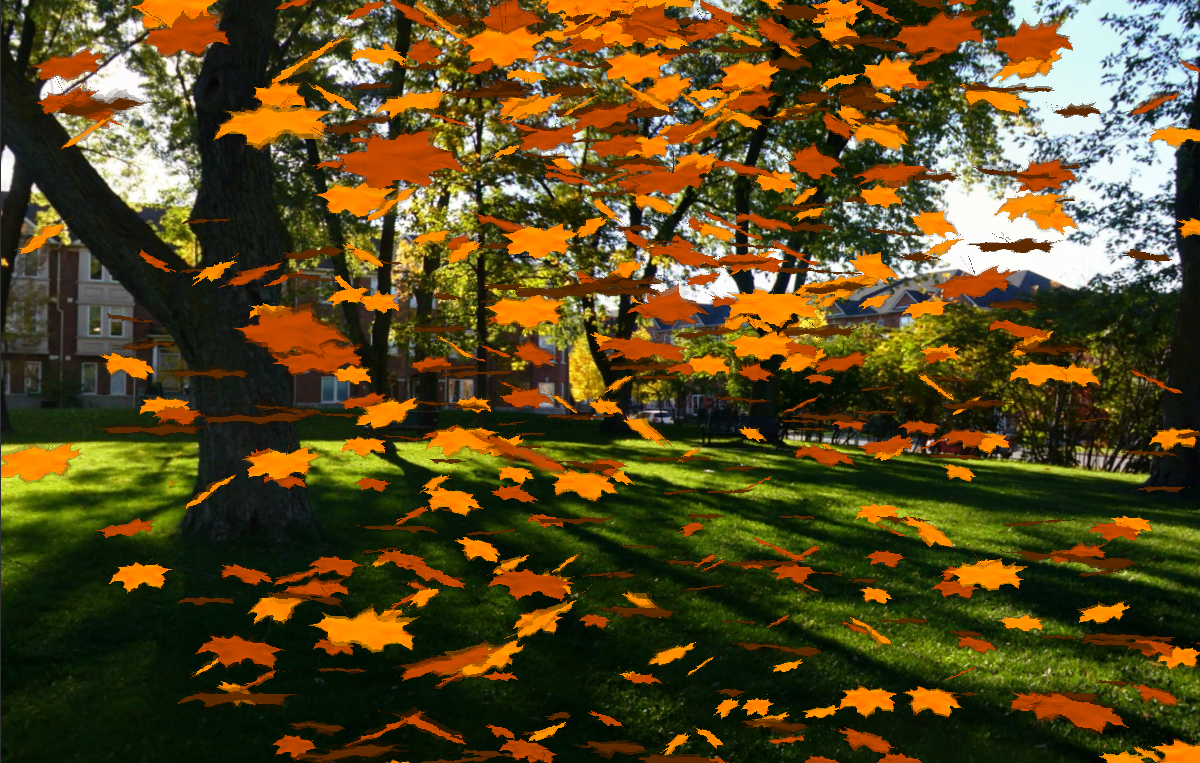
\includegraphics[width=1.0\textwidth]{obrazky-figures/podzim.png}
	\caption{Scéna obsahující podzimní scenérii. Padající listy jsou vytvořeny pomocí částicového systému. Při pohybu rotují a krouží po spirálovité dráze.}
	\label{fig:ps_podzim}
\end{figure}

Částice jsou rozšířeny několika způsoby. Při inicializaci každé částice se náhodně zvolí, kterou texturu bude využívat. Textura je zvolena vztahem \ref{eq:rand_index}, který vychází z~maximálního počtu textur. Funkce \texttt{rand()} vrací náhodné celé kladné číslo. Je tak možné přidat další generátory bez nutnosti měnit implementaci částice.
\begin{equation}
    \label{eq:rand_index}
    \text{ textureIndex} = rand() \text{ } mod \text{ maxTextures} 
\end{equation}

Souřadnice $x$ a $z$ jsou určeny náhodně a souřadnice $y$ je konstantní. Částice jsou tak generovány na čtvercové ploše. Modifikován je i pohyb částic. Ke směrovému vektoru gravitace je při každém kroku přičítána hodnota $w$, jenž je určena vztahem \ref{eq:sin_movement}. Její sinusový průběh závislý na čase dodává částici efekt spirálového pohybu. Hodnota $\alpha$ určuje rychlost změny a hodnota $\beta$ její sílu. Během pohybu ještě částice vertikálně rotují náhodnou rychlostí. Rotace je uskutečněna pomocí změny souřadnice $u$ při každém kroku simulace. 
\begin{equation}
    \label{eq:sin_movement}
    w = sin(time \times \alpha) \times \beta
\end{equation}

\subsection*{Vesmírná flotila}
Tato scéna znázorňuje flotilu vesmírných lodí. Lze ji nalézt na obrázcích \ref{fig:ps_flotila}. Implementací se jedná o~velmi podobnou scénu jako scéna \emph{Podzim}. Jejím cílem je demonstrovat možné využití navrhované metody a její nároky na výkon.
\begin{figure}[H]
	\centering
	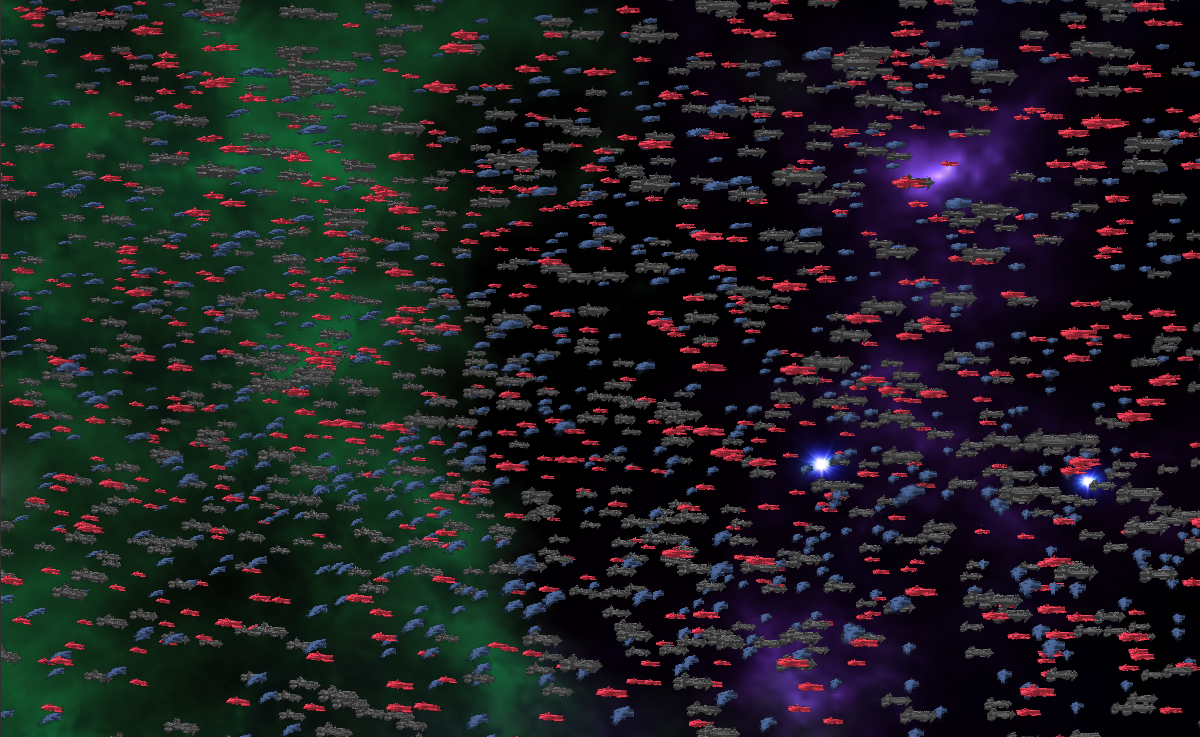
\includegraphics[width=0.7\textwidth]{obrazky-figures/flotila.png}
	\vspace*{1cm}
	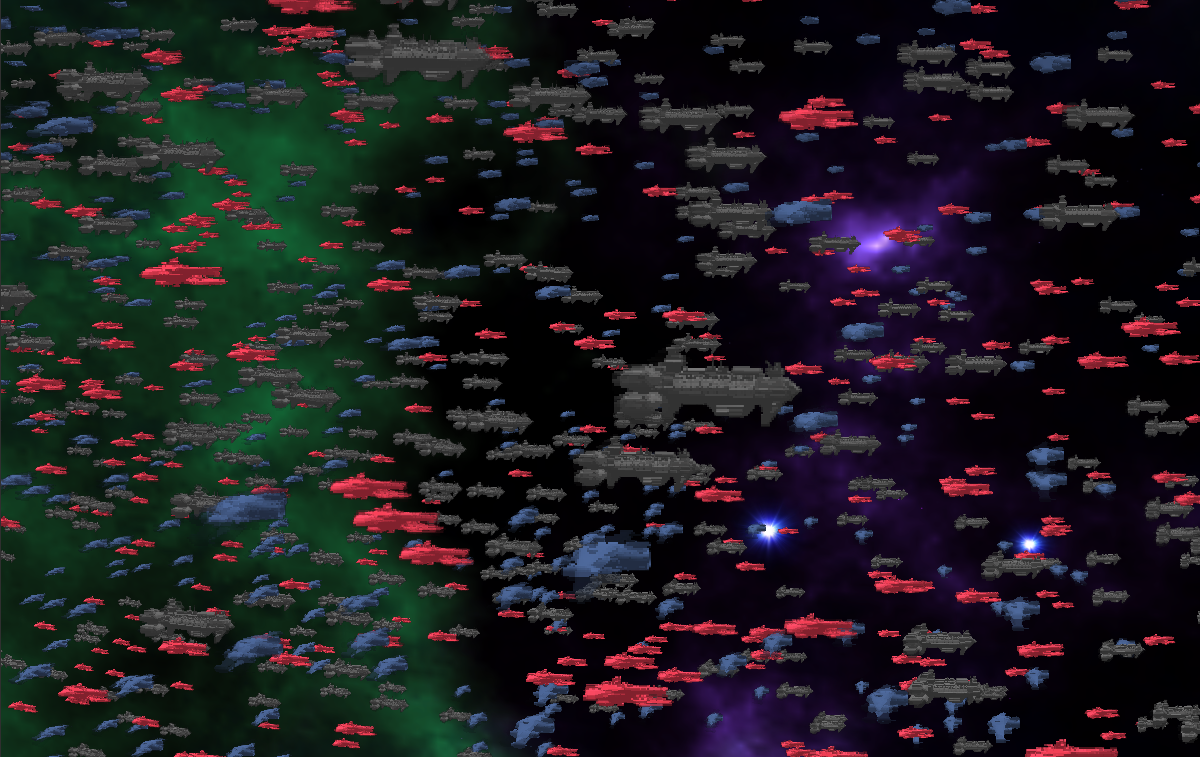
\includegraphics[width=0.7\textwidth]{obrazky-figures/flotila_detail.png}
	\caption{Scéna obsahující \emph{Vesmírnou flotilu}. Každý typ lodě je vytvořena z~jednoho ze tří objektů. Všechny částice se pohybují konstantní rychlostí totožným směrem. Na druhém obrázku se nachází detail částic, které tvoří částicový systém \emph{Vesmírná flotila}. Rozlišení textury light fieldu je 5000 pixelů a hustota je 31.}
	\label{fig:ps_flotila}
\end{figure}


Byly použity tři generátory se standardními modely. Každý model je vytvořen jiným objektem. Tyto se skládají přibližně z~123~000, 112~000 a 7~000 trojúhelníků. Scéna ve výchozím stavu obsahuje 5~000 částic, avšak při testování na výkonnější sestavě bylo dosaženo i 20~000 částic. Měření výkonu je věnována kapitola \ref{sec:mereni}.

Částice jsou opět rozšířeny o~náhodnou volbu textury popsanou vztahem \ref{eq:rand_index}. Počáteční souřadnice částice jsou určeny náhodně z~určitého rozsahu. Částice jsou tedy vytvářeny v~krychlovitém prostoru. Jejich pohyb není určen gravitací, pohybují se rychlostí, která je při zrození částice náhodně určena a poté zůstává konstantní.




\subsection*{Transformace}
V~obou předchozích scénách byla používaná textura určena při zrodu částice. Tato scéna však demonstruje možnost změny v~průběhu života částice. Byly použity dva generátory, jeden pro texturu krychle a druhý pro torus. Při zrodu částice využívá texturu krychle a při průchodu plochou, jež se nachází ve středu obrazovky, dojde k~přepnutí textury. Částice jsou také při zrodu náhodně rotovány, ale rychlost rotace je nulová. Tuto scénu lze nalézt na obrázku \ref{fig:ps_transformation}.

\begin{figure}[H]
	\centering
	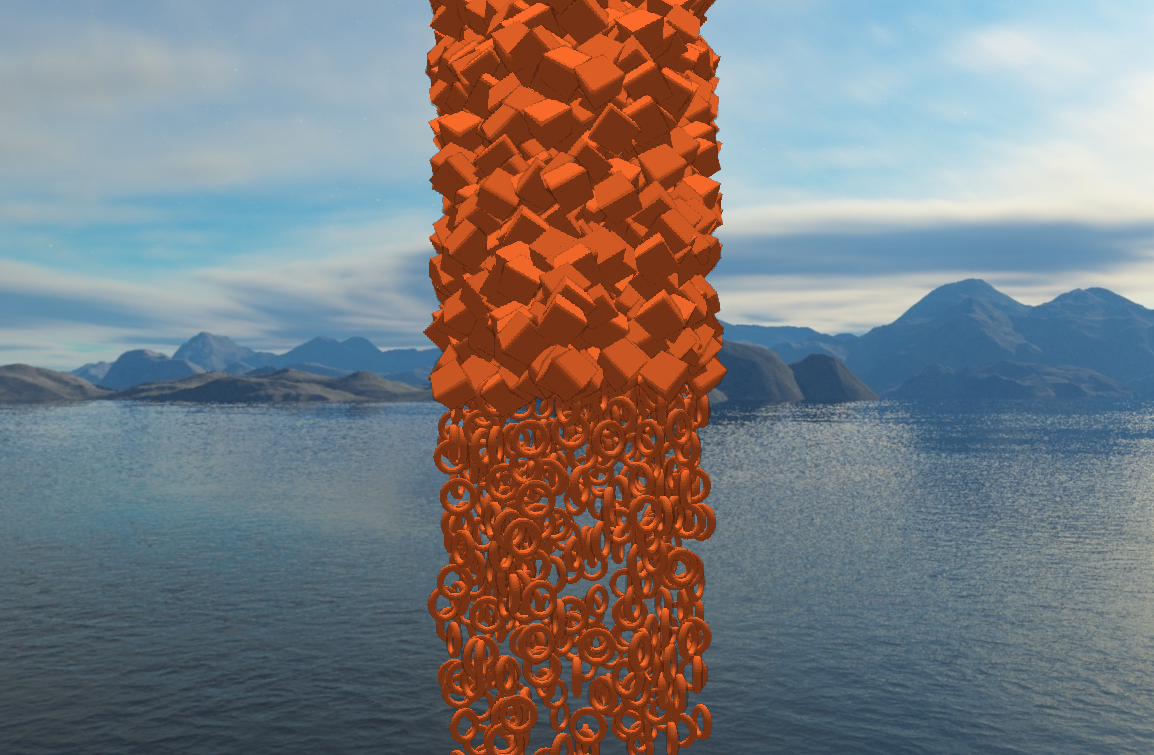
\includegraphics[width=1.0\textwidth]{obrazky-figures/transformace.png}
	\caption{Částicový systém, ve kterém se částice po průniku plochou ve středu obrázku transformují. }
	\label{fig:ps_transformation}
\end{figure}
\subsection*{Slunečnicové pole}
Scéna \emph{Slunečnicové pole} je odlišná od ostatních v~tom, že částice se nijak nepohybují a nemají dobu života. Jsou umístěny na čtvercovou plochu s~konstantní  souřadnicí $y$. Částice jsou také náhodně rotovány. 

Tato scéna využívá pouze jeden generátor. V~průběhu simulace probíhá cyklus dne a noci, což je znázorněno změnou skyboxu. Ukázka částicového systému a jeho změny se nachází na obrázku \ref{fig:ps_slunecnice}. Slunečnice jsou v~noci skleslé a ve dne směřují ke slunci. Tato transformace je uskutečněna tak, že je změněn model generátoru, což vede k~vyresetování \texttt{Cache tabulky} a následnému překreslení light fieldu. Je tak demonstrováno dynamické překreslování light fieldu.
\begin{figure}[H]
	\centering
	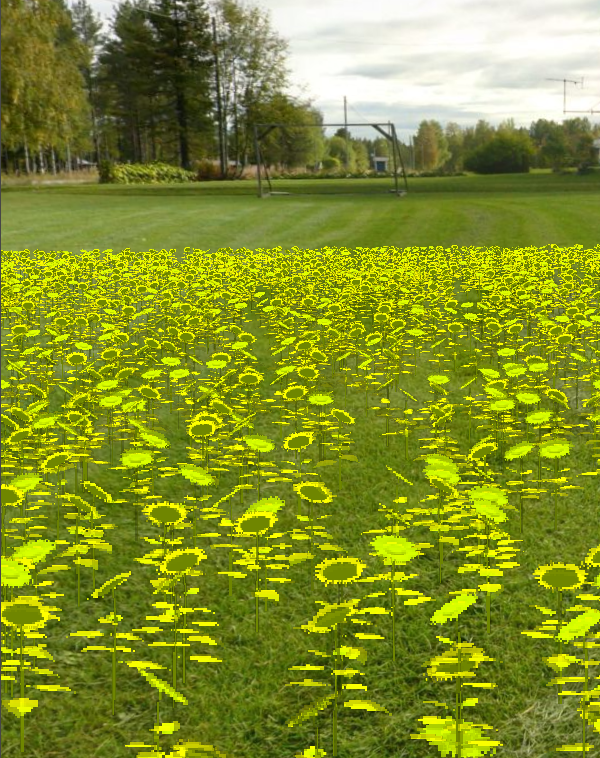
\includegraphics[width=0.45\textwidth]{obrazky-figures/slunecnice_den.png}
	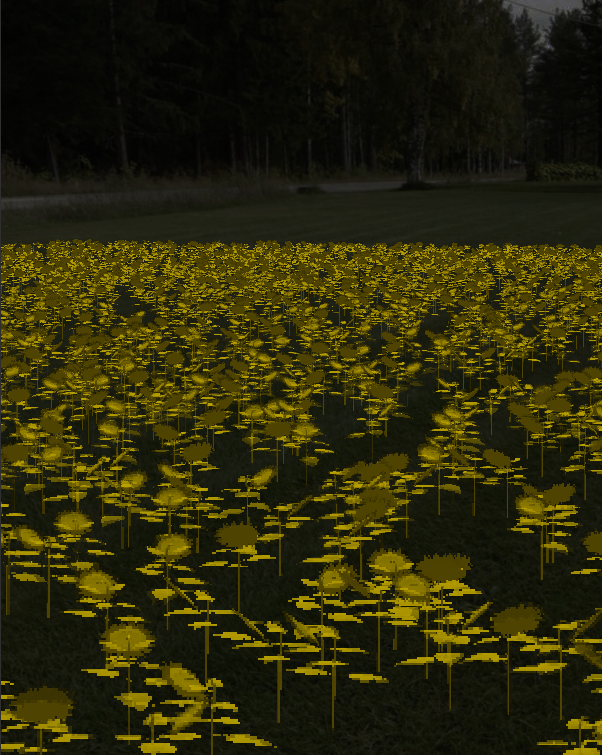
\includegraphics[width=0.45\textwidth]{obrazky-figures/slunecnice_noc.png}
	\caption{Částicový systém \emph{Slunečnicové pole}. Vlevo se nachází systém ve dne, kdy jednotlivé slunečnice směřují ke slunci. Pravý částicový systém se nachází v~noční fázi denního cyklu a slunečnice jsou tak skleslé. }
	\label{fig:ps_slunecnice}
\end{figure}

\subsection*{Disco}
Na obrázku \ref{fig:ps_disco} lze vidět další scénu demonstrující dynamické překreslování light fieldu. Systém se skládá z~velkého množství částic, které se pohybují podle směru gravitace. Je použit pouze jeden generátor se standardním modelem. V~krátkých pravidelných intervalech je měněno statické světlo modelu a jelikož se jedná o~\emph{Speciální parametr}, je vyresetována \texttt{Cache tabulka} a light field textura je opětovně generována. 

\begin{figure}[H]
	\centering
	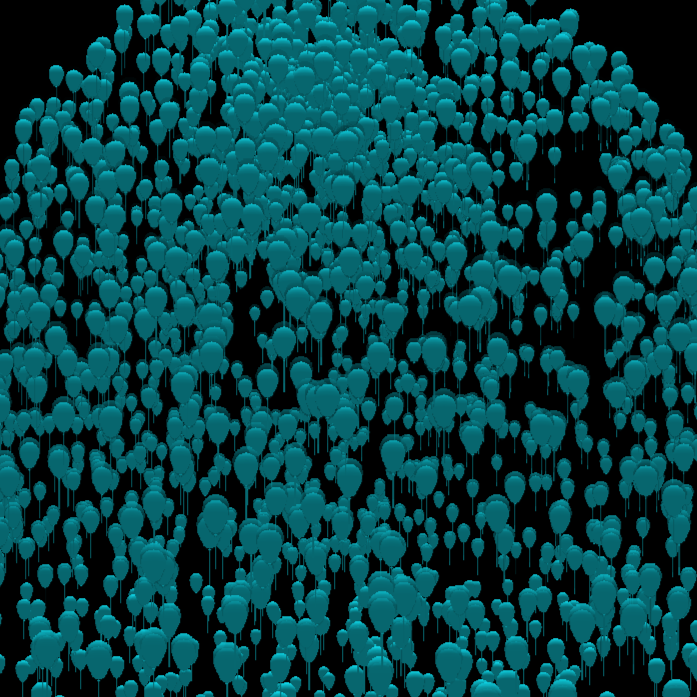
\includegraphics[width=0.24\textwidth]{obrazky-figures/disco1.png}
	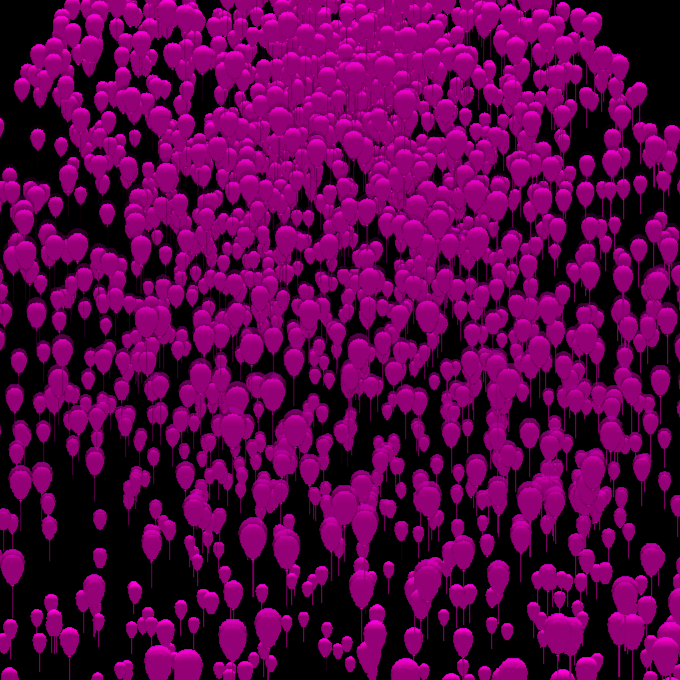
\includegraphics[width=0.24\textwidth]{obrazky-figures/disco2.png}
	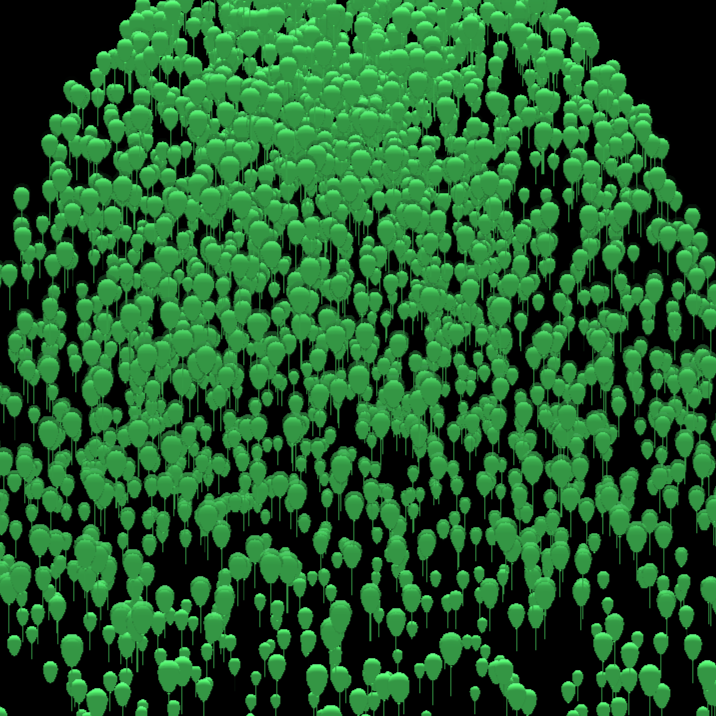
\includegraphics[width=0.24\textwidth]{obrazky-figures/disco3.png}
	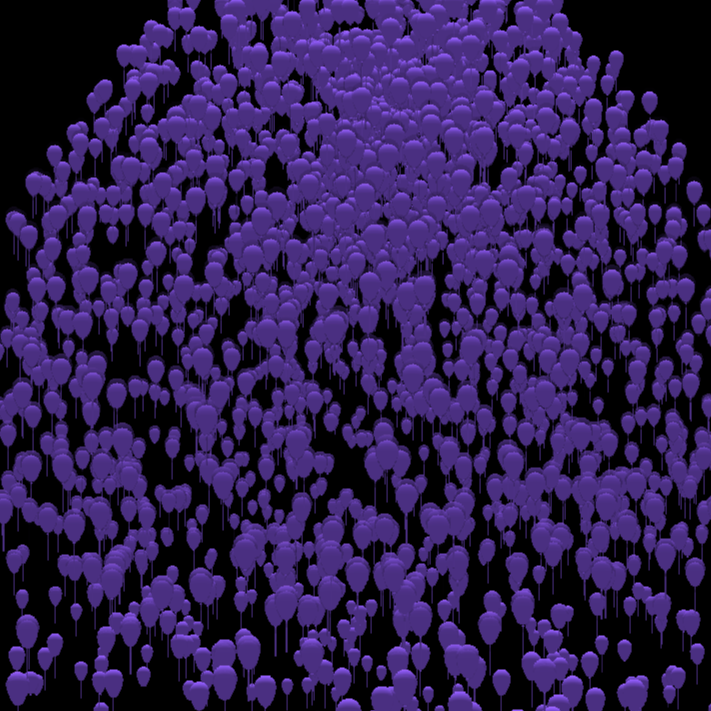
\includegraphics[width=0.24\textwidth]{obrazky-figures/disco4.png}
	\caption{Částicový systém náhodně měnící barvu v~krátkých časových intervalech. Systém využívá pouze jeden generátor, který je neustále překreslován.}
	\label{fig:ps_disco}
\end{figure}

\subsection*{Dynamické světlo}
\label{sec:real_light_scene}
Tato scéna demonstruje použití shaderu využívající dynamické světlo. Ve scéně jsou použity dva generátory. První generátor využívá obyčejný model a druhý využívá rozšířený model generující objekt s~normálami popsaný v~sekci \ref{sec:implemented_extensions}. Částice jsou tak osvětlovány v~reálném čase, a tak je možné pozorovat změnu osvětlení v~závislosti na pozici částice, což je znázorněno na obrázku \ref{fig:rel_light}
\begin{figure}[H]
	\centering
	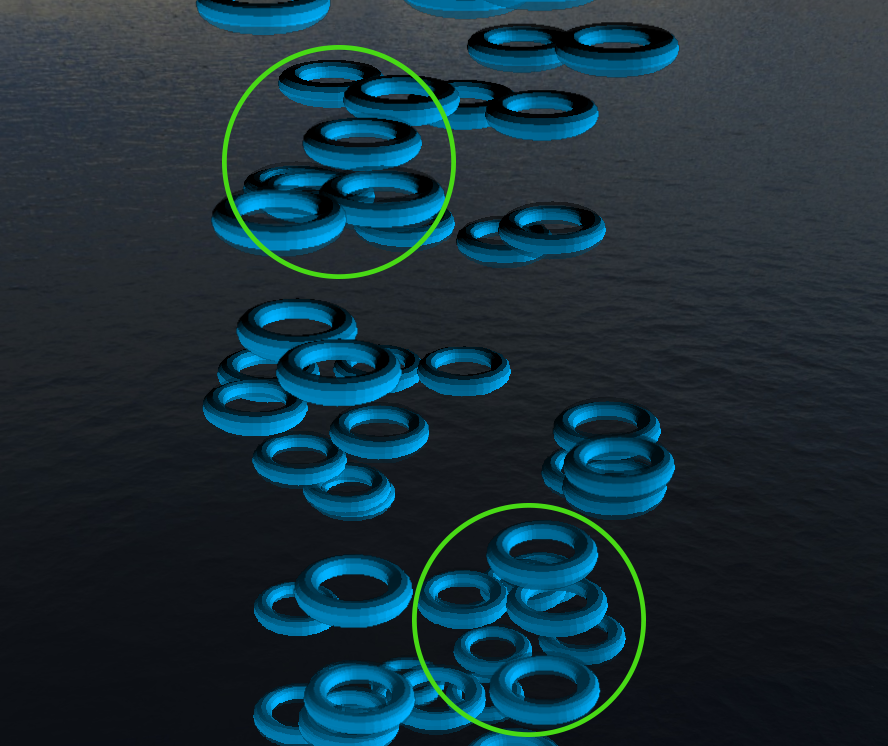
\includegraphics[width=0.7\textwidth]{obrazky-figures/dynamic_light.png}
	\caption{Částicový systém využívající dynamické světlo. V~horní označené oblasti je možné sledovat stín, jelikož se částice nachází nad zdrojem světla. V~dolní označené oblasti se tento stín nenachází, jelikož byla částice částečně osvícena.}
	\label{fig:rel_light}
\end{figure}
\subsection*{Scény pro měření}
V~nástroji je implementováno několik scén určených pro měření. Některé scény nejsou díky vysokým výkonnostním nárokům přístupné přes grafické rozhraní a je nutné je aktivovat přes CLI. Parametry těchto scén, jako jsou například počet částic, či rozlišení light field textury, je také možné měnit pomocí rozhraní z~příkazové řádky. 

Scény nazývané \textbf{Benchmark Basic} a \textbf{Benchmark Complex} obsahují totožné částicové systémy avšak různé modely. První zmíněná scéna obsahuje model s~objektem o~velikosti 3 476 trojúhelníků a druhý velmi složitý objekt obsahující 144 046 trojúhelníků.

Scény \textbf{Standard3D Basic} a \textbf{Standard3D Complex} využívají speciálního částicového systému, jenž nevyužívá light field renderingu, ale standardních renderovacích technik a instancování. Tento částicový systém je implementován třídou \texttt{standard3DParticles} a je popsán v~sekci \ref{sec:impl_particles}. Pro obě scény byly použity stejné modely jako u~jejich light field variant. To stejné platí i pro simulační část. 

Poslední scénou určenou pro měření je \textbf{Benchmark Disco}. Jedná se o~upravenou scénu \emph{Disco} pro účely měření. Parametry simulace byly nastaveny tak, aby odpovídaly ostatním měřícím scénám a scéna tak mohla být porovnávána s~ostatními. 
\section{Testovací nástroj}
\label{sec_benchmark_impl}
Cílem testovacího nástroje je provést měření popsané v~sekci \ref{sec:methodology} a výsledky zaznamenat. Nástroj také umožňuje analýzu těchto výsledků. Byl rozdělen na dva oddělené skripty sloužící k~různým účelům. Oba skripty byly implementovány v~jazyce \texttt{Python}.

Skript \texttt{benchmark.py} slouží k~samotnému měření. Spouští hlavní aplikaci s~různými parametry a zaznamenává měřené metriky. Výstup poté uloží do souboru pro pozdější analýzu. Skript spouští aplikaci s~různými parametry, které určují scénu, počet částic, rotaci scény a případné rozlišení light field textury. K~práci s~procesem aplikace byla použita knihovna \texttt{psutil}. Knihovna také umožňuje sledovat využití CPU či kolik RAM proces využívá. Ke sledování grafické karty byla použita knihovna \texttt{GPUtil}, jenž využívá nástroj \texttt{nvidia-smi}. Skript je tedy schopný pouze měřit metriky od společnosti \texttt{Nvidia}. Pro práci s~daty a jejich uložení byla použita knihovna \texttt{pandas}.

Skript \texttt{analyzer.py} slouží k~analýze naměřených dat. Data jsou načtena ze souboru, kde byla vytvořena prvním skriptem. Pro agregaci a jiné datové operace byla také použita knihovna \texttt{pandas}. Výsledné grafy jsou vytvořeny za pomocí knihovny \texttt{Matplotlib}.

Měřící skript byl pomocí nástroje \texttt{pyinstaller} převeden na spustitelný binární soubor. Takový sobor nevyžaduje, aby na sestavě, na které je měření prováděno, byly nainstalovány potřebné závislosti. Měření je tak možné provést bez jakékoliv instalace.



\chapter{Měření}
Tato kapitola se zaměřuje na analýzu výsledků měření, které byly provedeny pomocí měřícího nástroje. Metodika i měřené metriky jsou popsány v~sekci \ref{sec:methodology}. Konkrétní použité sestavy lze nalézt v~tabulce \ref{tab:pcs}. Na všech bylo provedeno měření na stejné verzi aplikace. Sestava S1 reprezentuje starší výkonný hardware a obsahuje nejvíce VRAM. Sestava S2 reprezentuje střední třídu a soustava S3 moderní výkonný počítač. Poslední sestava S4 reprezentuje starší a nevýkonný hardware. Při měření nebyly sledovány teploty, a tedy případné přehřívání komponent mohlo ovlivnit výsledky. To platí především pro sestavy S2 až S4, jelikož se jedná o~laptopy. 

\begin{center}
\begin{table}[h!]
\centering
\begin{tabular}{|l|l|l|l|}
\hline
\textbf{Sestava} & \textbf{CPU} & \textbf{GPU} & \textbf{VRAM} \\ 
\hline
S1 & AMD Ryzen 5 3600  & Nvidia GeForce GTX 1080 & 8 GB GDDR5X \\ 
S2 & Intel i5 9300H & Nvidia GeForce GTX 1650 L & 4 GB GDDR5  \\ 
S3 & AMD Ryzen 7 5800H  & Nvidia GeForce GTX 3060 L & 6 GB GDDR6 \\ 
S4 & Intel i5 8250U  & Nvidia GeForce MX150 L & 4 GB GDDR5 \\ 
\hline
\end{tabular}
\label{tab:pcs}
 \caption{Hardwarové specifikace jednotlivých měřených sestav. Značka L znamená, že se jedná o~verzi GPU pro laptopy.}
\end{table}
\end{center}

\section{Vizuální srovnání}
Vzhled částic vykreslovaných pomocí light fieldu značně ovlivňuje hustota a rozlišení textury. Nevhodná volba těchto parametrů může negativně ovlivnit vzhled částic. Rychlost pohybu může také ovlivňovat působení částice, jelikož plynule přechází mezi jednotlivými vzorky. Při nízké hustotě může být tedy nedostatečné vzorkování obzvláště patrné. Vzdálenost částice od kamery má také velký vliv na její vzhled, jelikož například nízké rozlišení není tak výrazné. 

Příliš nízká hustota způsobuje vizuální artefakty způsobené nedostatečným vzorkováním. V~takovém případě je rozdíl mezi jednotlivými snímky příliš vysoký a interpolace je tak až moc patrná. Zvýšení hustoty tento problém potlačí, avšak příliš vysoká hustota má velmi negativní dopad na výslednou kvalitu. Pokud například má textura light filedu rozlišení 5100 pixelů a hustota je 51, tak výsledná textura bude mít rozlišení pouze 100 pixelů. Tento problém lze řešit pomocí zvýšení rozlišení textury light fieldu, což má však negativní dopady na vytížení paměti grafické karty. Artefakty způsobené interpolací jsou však viditelné vždy a jejich zřetelnost lze jen redukovat. 

Tento jev lze sledovat na obrázcích \ref{fig:density_visual}. Zvýšení hustoty sice vyřešilo problém příliš viditelné interpolace kvůli nedostatečnému vzorkování, avšak tímto bylo výsledné rozlišení částice výrazně sníženo.  

\begin{figure}[H]
	\centering
	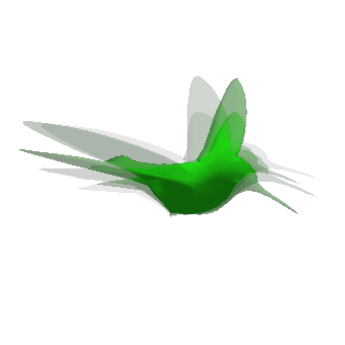
\includegraphics[width=0.32\textwidth]{obrazky-figures/density_l1.png}
	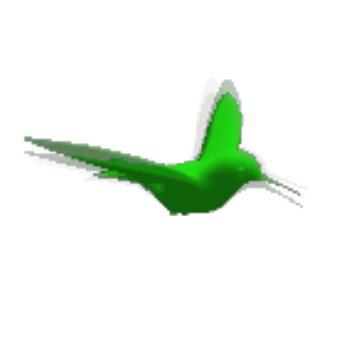
\includegraphics[width=0.32\textwidth]{obrazky-figures/density_l2.png}
	
\includegraphics[width=0.32\textwidth]{obrazky-figures/density_l3.png}

	\caption{Vliv hustoty textury light fieldu na vizuální artefakty a rozlišení. Kamera se nachází mezi dvěma vzorky a vzniká tak ghousting způsobený interpolací. Na levém obrázku má částice hustotu 11, na prostředním 31 a na posledním 51. Rolišení této textury je 5000 pixelů.}
	\label{fig:density_visual}
\end{figure}

Vliv textury na vizuální kvalitu částice je naznačen na obrázcích \ref{fig:texture_visual}. 
\begin{figure}[H]
	\centering
	
\includegraphics[width=0.32\textwidth]{obrazky-figures/texture_l1.png}
	
\includegraphics[width=0.32\textwidth]{obrazky-figures/texture_l2.png}
	
\includegraphics[width=0.32\textwidth]{obrazky-figures/texture_l3.png}

	\caption{Vliv rozlišení textury na vzhled částice. Levý obrázek zobrazuje částici, kde je rozlišení textury light fieldu 1000 pixelů. Na prostředním obrázku je toto rozlišení 2500 pixelů a na posledním 5000 pixelů. Hustota všech těchto textur je 31.  }
	\label{fig:texture_visual}
\end{figure}

Na obrázcích \ref{fig:comp_zoomed} lze pozorovat částici vykreslenou pomocí light fieldu a částici vykreslenou standardním způsobem. Lze zde pozorovat mírné rozostření celého modelu a vizuální artefakty nacházející se především u~okrajů modelu. Částice jsou obvykle pozorovány při pohybu a ze větší vzdálenosti, což výrazně potlačí viditelnost těchto vizuálních defektů. 
\begin{figure}[H]
	\centering
	
\includegraphics[width=0.45\textwidth]{obrazky-figures/bunny_nolightfield.png}
	
\includegraphics[width=0.45\textwidth]{obrazky-figures/bunny_lightfield.png}
	\caption{Na levém obrázku se nachází objekt \emph{Standford bunny} vykreslený pomocí standardního renderování. Vpravo se nachází stejný objekt vykreslený pomocí light fieldu. Hustota pořízené textury je 51 a rozlišení textury je 20 000 pixelů. Tyto hodnoty byly zvoleny tak, aby byl model co vizuálně nejpodobnější. Hodnoty jsou velmi vysoké a pro částicové systémy v~implementovaných scénách jsou výrazně nižší.  }
	\label{fig:comp_zoomed}
\end{figure}
Srovnání, které více odpovídá reálnému použití, lze nalézt na obrázcích \ref{fig:comp_particles}. Jeden částicový systém využívá třídu \texttt{standard3DParticles} a druhý navrhovanou metodu. Oba využívají stejný simulátor, takže částice se pohybují totožným způsobem. Podobnost těchto obrázků byla měřena pomocí metod MSE, PSNR a SSIM. Výsledky a srovnání s~obrázkem náhodného šumu lze nalézt v~tabulce \ref{tab:psnr_comp}.

\begin{figure}[H]
	\centering
	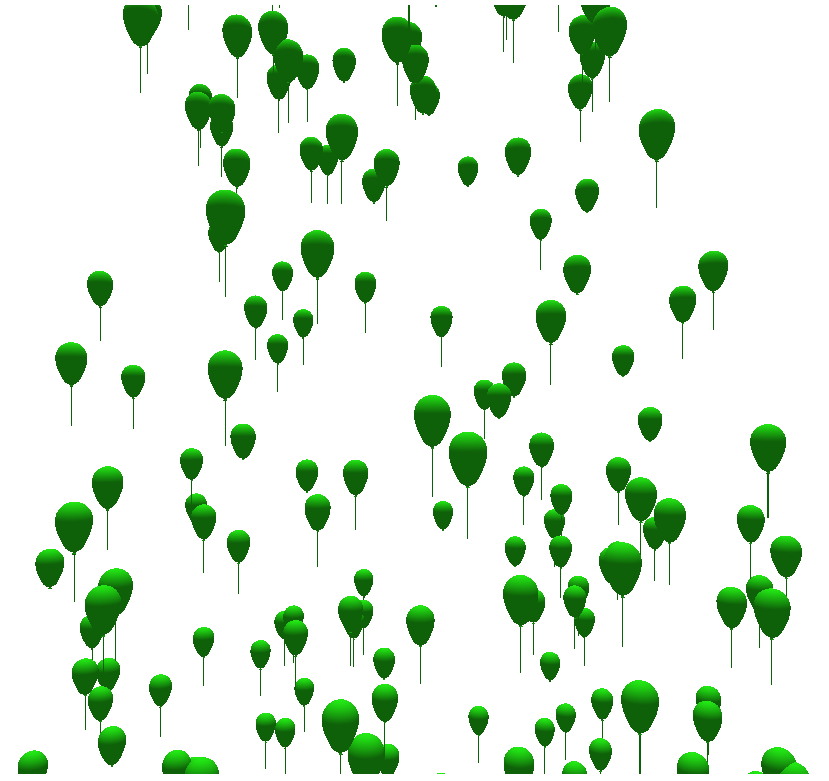
\includegraphics[width=0.45\textwidth]{obrazky-figures/nolightfield.png}
	\hspace*{1cm}
	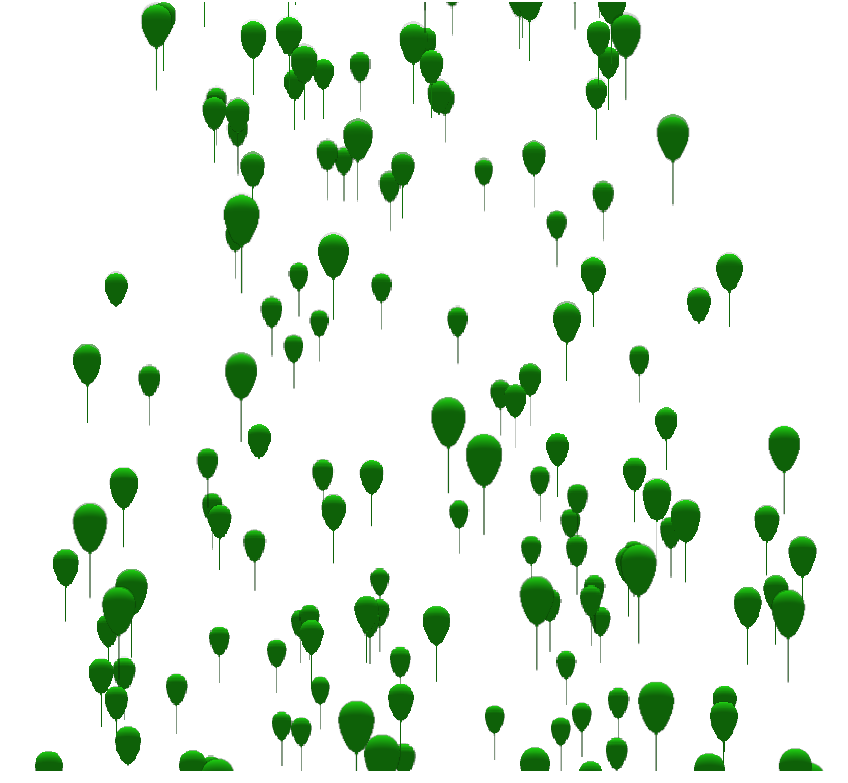
\includegraphics[width=0.45\textwidth]{obrazky-figures/lightfield.png}
	\caption{Na levém obrázku se nachází částicový systém nepoužívající light fieldu. Na druhém se nachází totožný částicový systém, který ale využívá navrhovanou metodu. }
	\label{fig:comp_particles}
\end{figure}

\begin{center}
\begin{table}[h!]
\centering
\begin{tabular}{|l|l|l|l|}
\hline
\textbf{Metoda} & \textbf{Obrázek A} & \textbf{Obrázek B} & \textbf{Výsledek} \\ 
\hline
MSE & standardní 3D & Light field & 556 \\
MSE & standardní 3D & Šum & 31 275 \\
PSNR & standardní 3D & Light field & 20.6 db \\
PSNR & standardní 3D & Šum  & 3.1 db \\
SSIM & standardní 3D & Light field & 92.3 \% \\
SSIM & standardní 3D & Šum  & 0.002 \% \\
\hline
\end{tabular}
\label{tab:psnr_comp}
 \caption{Srovnání snímků obrazovky pořízeného z~nástroje. Obrázek standardní 3D obsahuje částicový systém nevyužívající light field. Obrázek Light field obsahuje snímek částicového systému zobrazovaného pomocí navrhované metody. Poslední obrázek obsahuje pouze šum a slouží jako referenční hodnota.}
\end{table}
\end{center}
\section{Výkonnostní srovnání}
Tato sekce se zaměřuje na měření výkonnostních  nároků navrhované metody. Z~měřených sestav měla ve většině případů nejlepší výsledky soustava S1, což ukazuje závislost na výkonu grafické karty, jelikož například sestava S3 měla více výkonný procesor a i přesto byly výsledky horší. 

\subsection*{Sestava S1}
Na obrázku \ref{fig:graphS1Basic} lze pozorovat výsledky měření na soustavě S1. Ve scéně s~obyčejným objektem je patrné značné zlepšení oproti scéně nevyužívající light field. Scéna s~velmi komplexním objektem nevykazuje výrazné zhoršení oproti jednoduchému. Scéna s~komplexním objektem nevyužívající light field naopak vykazuje naprostný propad počtu snímků. Scéna \emph{Disco}, kde se velmi často light field překresluje nevykazuje téměř žádný pokles snímků oproti ostatním light field scénám.

\begin{figure}[H]
	\centering
		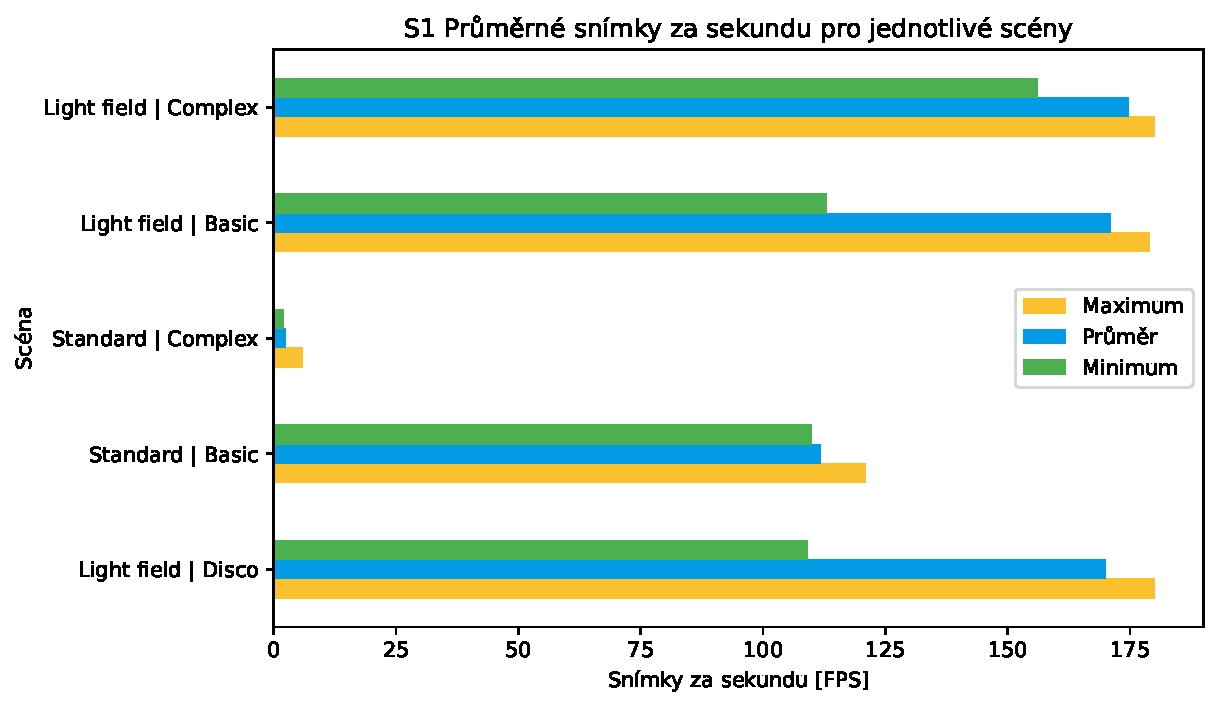
\includegraphics[width=0.88\textwidth]{obrazky-figures/graphS1basic.pdf}
	\caption{Graf znázorňující výsledky měření jednotlivých scén na sestavě S1.}
	\label{fig:graphS1Basic}
\end{figure}
Na grafu si lze také všimnout velmi výrazného rozdílu mezi minimem a průměrem u~scén s~light fieldem. Takový trend se projevuje i na všech ostatních sestavách. Tento pokles lze přisoudit nutnosti vytvoření textury a vygenerování většího počtu úhlů pohledu v~jednu chvíli (především při spuštění). Možným řešením by mohlo například být předvytvoření textury při inicializaci. Maximální počet snímků za sekundu je velmi blízký průměru, jelikož po úvodním zpomalení se vytížení příliš nemění. 

\subsection*{Sestava S2}
Sestava S2 dle grafů na obrázku \ref{fig:graphS2Basic} vykazuje obecně horší výsledky pro všechny scény, i přesto trendy jsou podobné. Poměr zvýšení počtu snímku scén s~a bez light fieldu zůstává také podobný. Rozdíl mezi minimem a průměrem u~scén s~light fieldem se ale výrazně snížil. To může být způsobeno například výrazně menším počtem shaderových výpočetních jednotek (640) grafické karty této sestavy, oproti sestavě S1 (2560), což může značně zpomalovat rychlost vertexového a především fragmentového shaderu částic. 
\begin{figure}[H]
	\centering
		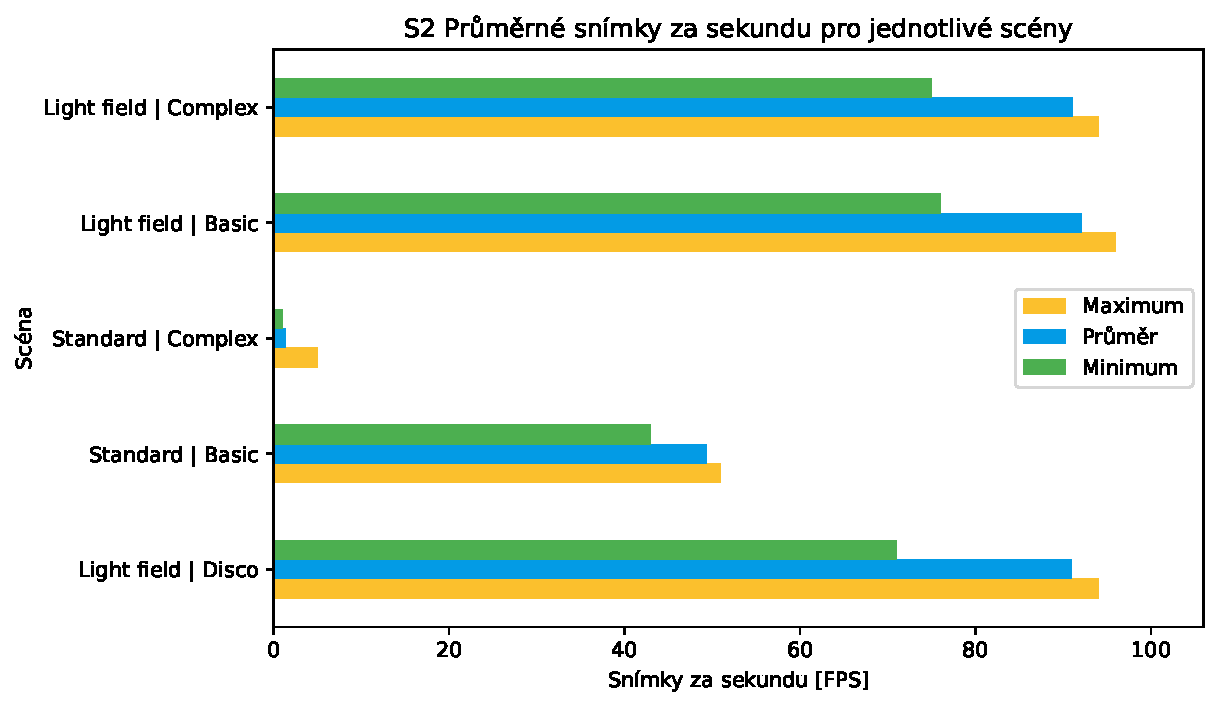
\includegraphics[width=0.88\textwidth]{obrazky-figures/graphS2basic.pdf}
	\caption{Graf znázorňující výsledky měření jednotlivých scén na sestavě S2.}
	\label{fig:graphS2Basic}
\end{figure}
\subsection*{Sestava S3}
Navzdory domněnce z~minulého  odstavce má sestava S3 s~větším počtem výpočetních jednotek (3840) horší výsledky než sestava S1. Tento jev je především výrazný při nižším počtu částic. To je možné přisoudit velmi vysokému rozdílu ve frekvenci taktu těchto grafických karet. GPU sestavy S1 má taktovací frekvenci 1600 MHz, zatímco grafická karta sestavy S3 má frekvenci 900 MHz. Naměřené výsledky je možné pozorovat v~grafu \ref{fig:graphS3Basic}.

\begin{figure}[H]
	\centering
		\includegraphics[width=0.88\textwidth]{obrazky-figures/graphS3basic.pdf}
	\caption{Graf znázorňující výsledky měření jednotlivých scén na sestavě S3.}
	\label{fig:graphS3Basic}
\end{figure}

\subsection*{Sestava S4}
Poslední sestava S4 byla ze všech nejméně výkonná, což se velmi znatelně projevilo na výsledcích, které lze nalézt v~grafu na obrázku \ref{fig:graphS4Basic}. Ani jedna ze scén nedosáhla na 60 snímků za sekundu. Avšak průměrný počet snímků ve scéně s~light fieldem byl stále dvojnásobný oproti scéně bez něj. Scéna s~komplexním objektem se bez light filedu nezvládla vykreslit a naměřená data jsou tak v~tomto případě spíše neplatná. Scéna s~komplexním modelem vykresleným pomocí light fieldu však opět dosáhla stejného počtu snímku jako scéna bez něj. Při menším počtu částic by tedy mohla být navrhovaná metoda výhodnější i pro takto nevýkonnou sestavu.  

\begin{figure}[H]
	\centering
		\includegraphics[width=0.88\textwidth]{obrazky-figures/graphS4basic.pdf}
	\caption{Graf znázorňující výsledky měření jednotlivých scén na sestavě S4.}
	\label{fig:graphS4Basic}
\end{figure}

\subsection{Vliv počtu částic}
Značně výrazný vliv na rychlost systému má počet částic. Větší počet částic nejenom ovlivňuje počet vertexů a fragmentů ve scéně, ale také velikost bufferů obsahujících pozici, uv souřadnice a textury. Především se zvyšuje počet přístupů k~textuře. 

V~grafu na obrázku \ref{fig:graph_particles} je možné sledovat, jak se počet snímků za sekundu snižuje s~přibývajícím počtem  částic. Tento pokles je nejdříve velmi prudký, s~větším počtem částic však zpomaluje, jelikož se částice začínají častěji překrývat. Pokles FPS je u~sestavy S3 pomalejší, než u~sestav S1 a S2. Toto může být způsobeno velkým počtem výpočetních jednotek, ale i například dostatečným chlazením.

Hodnoty nižší než 1 000 částic nebyly v~grafu zobrazeny, jelikož dosahovaly příliš vysokých hodnot. 
\begin{figure}[H]
	\centering
		\includegraphics[width=0.7\textwidth]{obrazky-figures/particle_count.pdf}
	\caption{Graf znázorňující vliv počtu částic ve scéně na počet snímků za sekundu (FPS). Rozlišení light fieldu textury je 1000 pixelů.}
	\label{fig:graph_particles}
\end{figure}

\subsection{Vliv rozlišení textury}
Další z~faktorů ovlivňující výkon je rozlišení textury. Příliš vysoké rozlišení může zcela zaplnit video paměť grafické karty a snížit tak výkon. Tento problém však značně redukuje \textbf{mipmapování}. Pokud je zapnuté, nemá zvyšující se kvalita textury téměř žádný vliv na výkon. Pokud není zapnuté, tak se počet snímků za sekundu snižuje s~přibývajícím rozlišením. Vliv mipmapingu lze sledovat na obrázku \ref{fig:graph_res_mipmapping}.


\begin{figure}[H]
	\centering
	\includegraphics[width=0.49\textwidth]{obrazky-figures/resolution_mipmaping_on2.pdf}
	\includegraphics[width=0.49\textwidth]{obrazky-figures/resolution_mipmaping_off2.pdf}

	\caption{Graf vlevo znázorňuje vliv rozlišení textury na FPS a na využití video paměti grafické karty. Graf vpravo vyobrazuje totéž, avšak s~vypnutou funkcí mipmaping. V~této scéně se nachází 3000 částic, obě měření proběhla na sestavě S1.}
	\label{fig:graph_res_mipmapping}
\end{figure}

V~praxi je nutné rozlišení textury snížit co nejvíce, a to i když není výkon snížen, jelikož může vykreslování scény vyžadovat paměť i na jiné objekty. Je vhodné také texturu označit za nerezidentní v~případě, že není viditelná, aby došlo k~uvolnění paměti. Snížení paměťových nároků lze také dosáhnout pomocí komprese, jelikož ta je na light field data velmi efektivní, jak je popsáno v~sekci \ref{sec:theory_create}.

\label{sec:mereni}

\chapter{Závěr}
Byla navrhnuta a implementována metoda kombinující částicové efekty a light field. Vznikl tak nástroj, který umožňuje jednoduše měnit parametry systému a přepínat implementované ukázkové scény. Tyto scény demonstrují různou funkcionalitu, jako je například dynamické generování light fieldu při běhu či využití několika různých light fieldů současně. Implementace byla rozdělena na oddělené moduly, které lze velmi jednoduše rozšiřovat o~další funkcionalitu, a snadno tak docílit požadovaného efektu.  

Následně byla metoda změřena, a to jak z~pohledu vizuálního, tak i výkonnostního. Měření ukázalo, že navrhnutá metoda může být značně efektivnější než standardní metody vykreslování. Například  na méně výkonné sestavě nebylo možné velmi komplexní objekt vykreslit standardní metodou v~reálném čase, zatímco při použití navrhované metody bylo dosaženo dostatečného počtu snímku za sekundu pro zobrazování v~reálném čase. Mohou však vznikat vizuální artefakty, které lze značně omezit vhodnou volbou parametrů. Měření také ukázalo velmi výraznou závislost na výkonu grafické karty, především na výkonu shaderových výpočetních jednotek. Pokud tedy budoucí vývoj hardwaru bude směřovat právě tímto směrem, lze předpokládat, že navrhovaná metoda se stane o~to relevantnější. 

Při reálném použití je nutné, aby uživatel správně zvolil, co opravdu potřebuje k~dosažení požadovaného efektu. Dynamické generování light fieldu nemusí být pro některé scény nutné a bylo by výhodnější light field předgenerovat. To stejné platí i pro použití několika light fieldů současně. Odstraněním této funkcionality se tak lze například vyhnout použití bindless textur, které nejsou na některém hardwaru podporované. 

Na práci lze v~budoucnu navázat například v~podobně výkonnostních  optimalizací. Simulace částic a výpočty $uv$ souřadnic jsou vypočítávány na procesoru, avšak pro tento účel by bylo možné implementovat výpočetní shader. Další vhodnou oblastí pro optimalizace je interpolace, jenž probíhá při zobrazování light fieldu. Samotné vykreslování light fieldu by mohlo být uskutečněno pomocí konečné hloubky ostrosti. Problematické je také použití sférického mapování textury, které není vhodné v~případě, kdy se může kamera dostat do blízkosti pólů koule.  

%===============================================================================
